%%  Chapter 4 - Results
% TODO: Abstract Fit: mention "asymmetric precipitation on windward
% slopes" in abstract, ensure include a figure for
% track_1_dpd_windward_leeward.png in Chapter 4 to support this claim.

%% TODO: add
% BOE mechanism determines which systems persist; show 4 signature"
% version:
% "Four independent observational signatures uniquely identify Brown
% Ocean Effect: sustained inner-core latent heat flux, progressive
% soil moisture wetting, dew-point depression suppression, and inward
% precipitation contraction. These signatures appear in all
% long-lived systems and absent in all short-lived systems,
% demonstrating that the BOE is the dominant mechanism. Eastern Ghats
% terrain cannot stop BOE-active systems, confirming that
% land-atmosphere coupling, not topography, determines post-landfall longevity."

\ifpdf
\graphicspath{{chapters/Figs/}{chapters/Figs/Raster/}{Figs/PDF/}{Figs/}}
\else
\graphicspath{{chapters/Figs/}{chapters/Figs/Vector/}{Figs/}}
\fi

\chapter{Results}
\label{ch:results}

\section{Multi-Year Climatological Patterns: 2001-2025}
\label{sec:results_multiyear}

% \subsection{Spatial Distribution of Track Termination: The Eastern
% Ghats Filter}
% \label{subsec:multiyear_spatial}
%
% Figure~\ref{fig:all_tracks_spatial} shows all confirmed MD tracks
% from 2001 to 2025, colour-coded by duration (hours). The spatial
% pattern of track termination points is the most direct visual
% evidence for the Eastern Ghats acting as a selective filter rather
% than an absolute barrier.
%
% % INSERT FIGURE - from Overall_years/ or plot_all_years.py
% %   All-track map, coloured by duration. Add Eastern Ghats 600m contour.
% %   Look for: Overall_years/all_tracks_2001_2025.png or similar.
% \begin{figure}[H]
%   \centering
%   \fbox{\rule{0pt}{8cm}\rule{0.90\textwidth}{0pt}}
%   % \includegraphics[width=0.90\textwidth]{Overall_years/all_tracks_2001_2025_by_duration}
%   \caption[All MD tracks, 2001-2025, coloured by post-landfall duration]{All
%     confirmed ERA5 Monsoon Depression tracks (2001-2025), colour-coded from
%     blue (short-lived, $<48$\,h post-landfall) through red (long-lived,
%     $\geq 96$\,h post-landfall). Eastern Ghats 600\,m elevation contour (bold
%     grey line) overlaid. The spatial clustering of track termination points is
%   a direct map of the terrain-filtering effect.}
%   \label{fig:all_tracks_spatial}
% \end{figure}
%
% From Figure~\ref{fig:all_tracks_spatial}, three spatial patterns are evident:
%
% \textbf{Pattern 1: Short-lived systems terminate east of the 600\,m
% contour.} The majority of short-lived MDs (blue-green tracks)
% dissipate within 200-400\,km of the coastline, with termination
% points clustering east of or within the Eastern Ghats terrain zone
% (600\,m contour). This clustering is consistent with Mechanism 4
% (vortex tilt decoupling; Section~\ref{subsec:ghats_mechanisms}):
% without BOE surface LHF to maintain boundary-layer convergence, the
% terrain-induced tilt increase is sufficient to cause structural
% collapse before or during the terrain crossing.
%
% \textbf{Pattern 2: Long-lived systems concentrate over the Gangetic
% plain west of the Ghats.} Long-lived tracks (orange-red) extend well
% west of the 600\,m contour into the Gangetic plain, eastern
% Rajasthan, and Madhya Pradesh. These tracks correspond to systems
% that successfully cleared the terrain and continued under BOE
% maintenance for multiple days. The spatial clustering of these
% long-lived tracks over the Gangetic plain is physically meaningful:
% this region has the highest climatological July-August \texttt{SWVL1}
% ($>0.35$\,m$^3$\,m$^{-3}$) in India due to its clay loam soils and
% high annual monsoon rainfall, precisely the conditions that enable
% and sustain the BOE.
%
% \textbf{Pattern 3: River-valley gap tracks achieve greater inland
% penetration.} A subset of long-lived tracks shows notably greater
% inland penetration distance than others with comparable ASMI values.
% Examining the landfall longitude of these outlier tracks reveals that
% they made landfall in alignment with the major river-valley gaps of
% the Eastern Ghats (the Mahanadi corridor near 84-85$^\circ$E, the
% Godavari corridor near 81-82$^\circ$E). Gap-aligned MDs experience
% smaller TSI values (lower terrain obstacle), preserving low-level BoB
% moisture inflow for longer through the terrain-crossing phase, and
% thus allowing the BOE to activate more efficiently on the leeward side.
%
% \subsection{Duration Distribution and the 96-Hour Threshold}
% \label{subsec:multiyear_duration}
%
% Figure~\ref{fig:duration_histogram} shows the frequency distribution
% of MD post-landfall durations across the 2001-2025 climatology. The
% distribution is strongly right-skewed, with a mode near 24-48 hours
% (reflecting the most common conventional post-landfall decay) and a
% pronounced tail extending beyond 96 hours. This bimodal character-a
% dominant short-duration peak and a secondary long-duration tail-is
% consistent with the BOE hypothesis imposing a threshold-type
% separation between two regimes rather than a continuous spectrum of behaviour.
%
% The threshold at 96 hours used to classify short- versus long-lived
% systems is not arbitrary: it corresponds approximately to the 85th
% percentile of the duration distribution, separating the bulk
% conventional decay population from the tail of anomalously persistent
% systems. Systems in this tail account for a disproportionately large
% fraction of total inland precipitation and flooding, despite
% constituting a minority of events.
%
% % FIX: duplicate label. But i need differnt figures as well
% % INSERT FIGURE - duration histogram
% %   Overall_years/duration_histogram.png from plot_all_years.py
% %   Show: bar chart with 24h bins, dashed line at 96h, label "96h threshold".
% %   Colour bars blue for < 96h and orange for >= 96h.
% \begin{figure}[H]
%   \centering
%   % \includegraphics[width=0.78\textwidth]{Overall_years/duration_histogram}
%   \fbox{\rule{0pt}{6cm}\rule{0.78\textwidth}{0pt}}
%   \caption[Frequency distribution of MD post-landfall duration, 2001-2025]{
%     Frequency distribution of MD post-landfall duration (hours) for
%     all 2001-2025
%     events. The right-skewed distribution with a tail beyond 96 hours
%     is consistent
%     with the BOE imposing a threshold separation between two distinct
%     decay regimes.
%     Blue bars: conventional decay ($<96$\,h); orange bars: long-lived systems
%   ($\geq 96$\,h, primary focus of this study).}
%   % \label{fig:duration_histogram}
% \end{figure}
%
% % \subsection{ASMI-Duration Relationship: 24-Year Statistical Evidence}
% % \label{subsec:multiyear_asmi}
% %
% % Figure~\ref{fig:asmi_vs_duration_scatter} presents the scatter of
% % 7-day ASMI against
% % post-landfall duration for all confirmed land-falling MDs in the
% % 2001-2025 dataset.
% % Each point represents one MD event; colour denotes BOE classification.
% %
% % % INSERT FIGURE - compute from antecedent_analysis.py
% % % outputs across all years
% % %   Scatter: x = ASMI_7d (m3/m3), y = post-landfall duration (h)
% % %   Colour: orange = BOE candidate, blue = non-BOE
% % %   Add: vertical dashed line at ASMI = 0.35, horizontal dashed line at 96h
% % %   Add: regression line + 95% CI band
% % \begin{figure}[H]
% %   \centering
% %   % \includegraphics[width=0.82\textwidth]{Overall_years/asmi_7d_vs_duration_scatter}
% %   \fbox{\rule{0pt}{7cm}\rule{0.82\textwidth}{0pt}}
% %   \caption[ASMI (7-day) vs post-landfall duration, all 2001-2025
% %   events]{7-day ASMI (m$^3$\,m$^{-3}$, horizontal axis) vs
% %     post-landfall duration (h, vertical axis) for all 2001-2025
% %     confirmed land-falling MDs. BOE candidates (orange); non-BOE
% %     systems (blue). Vertical dashed line at ASMI $=
% %     0.35$\,m$^3$\,m$^{-3}$ marks the approximate threshold above which
% %   BOE candidacy dominates.}
% %   \label{fig:asmi_vs_duration_scatter}
% % \end{figure}
% %
% % \yellownote{Look into this}
% % From Figure~\ref{fig:asmi_vs_duration_scatter}, the 25-year dataset
% % reveals the following
% % statistical regularities:
% % \begin{enumerate}
% %   \item \textbf{Positive ASMI-duration correlation:} Pearson $r =
% %     [r_1]$, $p = [p_1]$ (effective sample size corrected following
% %     \citealt{bretherton1999effective}). Higher antecedent soil
% %     moisture is significantly associated with longer post-landfall
% %     duration across the full climatological record, confirming the
% %     ASMI as a statistically valid predictor.
% %   \item \textbf{Threshold behaviour near 0.35\,m$^3$\,m$^{-3}$:}
% %     Systems with ASMI$_{7d}$ $> 0.35$ are predominantly long-lived
% %     and BOE-candidate. Below this threshold, the vast majority are
% %     short-lived. This threshold corresponds to the critical soil
% %     moisture level at which hydraulic conductivity drops steeply in
% %     Gangetic clay loam \autocite{clapp1978empirical,
% %     seneviratne2010investigating}, marking the transition from
% %     water-limited to energy-limited evaporation.
% %   \item \textbf{Scatter within each ASMI class:} The scatter around
% %     the regression line is substantial, indicating that ASMI alone
% %     does not fully explain duration variability. The residual
% %     variance is likely attributable to differences in terrain
% %     exposure (TSI), track alignment with river-valley gaps, and the
% %     intensity of the MD at landfall. This residual structure
% %     motivates the combined ASMI + TSI predictor framework discussed
% %     in Chapter~\ref{ch:discussion}.
% % \end{enumerate}
%
% % \subsection{Terrain Sensitivity Index vs Duration: The Terrain Filter}
% % \label{subsec:multiyear_tsi}
% %
% % Figure~\ref{fig:tsi_vs_duration} shows the relationship between
% % track-mean Terrain
% % Sensitivity Index (TSI) and post-landfall duration for the subset
% of MDs that
% % crossed the Eastern Ghats.
% %
% % \yellownote{TODO}
% % % INSERT FIGURE - from elevation_metrics.csv (all years)
% % %   Scatter: x = mean track TSI, y = post-landfall duration (h)
% % %   Colour: orange = BOE candidate, blue = non-BOE
% % \begin{figure}[H]
% %   \centering
% %   % \includegraphics[width=0.80\textwidth]{Overall_years/tsi_vs_duration_scatter}
% %   \fbox{\rule{0pt}{6.5cm}\rule{0.80\textwidth}{0pt}}
% %   \caption[Terrain Sensitivity Index vs post-landfall duration, all
% %   Ghats-crossing MDs]{
% %     Track-mean TSI vs post-landfall duration for all Ghats-crossing
% %     MDs in 2001-2025. BOE candidates (orange) cluster in the low-TSI,
% %     high-duration quadrant; non-BOE systems (blue) are distributed
% %     across all TSI values, confirming that terrain sensitivity is a
% %     decay-promoting factor but that BOE can overcome
% %   moderate terrain barriers.}
% %   \label{fig:tsi_vs_duration}
% % \end{figure}
% %
% % The key observation from Figure~\ref{fig:tsi_vs_duration} is the in
% % the distribution: BOE candidates cluster almost exclusively in the
% % low-TSI, high-duration quadrant (lower-right), while non-BOE systems
% % populate the full TSI range, including both low and high TSI values.
% % This pattern supports the interpretation that:
% %
% % \begin{enumerate}
% %   \item High TSI alone is sufficient to produce short duration
% %     (upper-left quadrant), regardless of BOE status-the terrain is
% %     too severe even for BOE to compensate.
% %   \item Low TSI with high ASMI (BOE candidate) produces long duration
% %     (lower-right).
% %   \item Low TSI with low ASMI (non-BOE) can still produce short
% %     duration, because the limiting factor is the surface moisture
% %     state, not the terrain.
% % \end{enumerate}
% %
% % This three-way interaction (ASMI, TSI, and their joint effect) is the
% % most complete statistical summary of the terrain-BOE modulation of MD
% % inland longevity that this dataset permits. A composite index
% % combining ASMI$_{7d}$ and TSI$^{-1}$ as a product may provide
% % improved predictive skill relative to either variable alone, and is
% % identified as a recommendation for operational forecasting research
% % (Section~\ref{sec:conclusions_operational}).
% %
% % \subsection{Orographic Blocking Factor and Speed Reduction}
% % \label{subsec:ghats_blocking_results}
% %
% % \yellownote{FIX: reference}
% % The translational speed profiles from \texttt{speed\_analysis.py}
% % provide the most direct observational measure of terrain-induced
% % blocking. Figure~\ref{fig:ts_speed_elev} shows that all
% % Ghats-crossing MDs decelerate as terrain elevation increases through
% % the 200-1000\,m zone, with mean speed reduction of approximately
% % $\Delta v \approx$ [X]\,km\,h$^{-1}$ at the 600\,m contour relative
% % to the pre-landfall ocean-phase speed. This deceleration is a direct
% % consequence of increased surface roughness and mechanical flow
% % blocking by the terrain - consistent with the Terrain Sensitivity
% % Index formulation (Section~\ref{sec:terrain_method}).
% %
% % The blocking effect is not uniform across the Ghats. Systems making
% % landfall between 84-87$^\circ$E (the Mahanadi corridor, near Odisha)
% % encounter lower mean TSI values and show smaller speed reductions
% % than those tracking through the southern Ghats (south of 16$^\circ$N,
% % high TSI). This longitude-dependent blocking is visible in
% % Figure~\ref{fig:elevation_comparison}: the scatter in per-track speed
% % reduction correlates with the landfall longitude, with gap-aligned
% % tracks showing shallower deceleration.
% %
% % The critical distinction between BOE-candidate and non-BOE systems is
% % not in the deceleration magnitude during the terrain crossing - both
% % categories slow at comparable rates within the 600-1000\,m elevation
% % zone. The difference appears on the leeward side: BOE-candidate
% % systems recover speed as terrain elevation drops below 200\,m, while
% % non-BOE systems continue to slow. This leeward speed recovery is
% % interpreted as evidence that sustained surface LHF (from the wet
% % leeward soil) maintains the low-level pressure gradient that drives
% % the system forward, whereas in non-BOE systems the pressure gradient
% % weakens as convective organisation collapses after terrain crossing.
%
% % \yellownote{TODO: add subsection on  the precipitation recycling ratio}
% % \subsection{Precipitation Recycling Ratio}
% % \label{Precipitation Recycling Ratio}
% %
% % The precipitation recycling ratio $\rho = E/P$ (where $E$ is local
% % evapotranspiration in mm\,h$^{-1}$ and $P$ is total precipitation) provides
% % an independent measure of how much of the MD's rainfall is
% sourced from local surface evaporation rather than large-scale
% moisture advection.
% Over the ocean  phase, $\rho \approx 0.05$-0.15, indicating that most
% precipitation comes from advected oceanic moisture. After landfall
% in BOE-candidate systems,
% % Figure~\ref{fig:track1_recycling} shows $\rho$ rising to
% 0.25-0.40, consistent with local surface evapotranspiration
% contributing a growing fraction of the
% % precipitation total. This elevated recycling ratio is a direct signature of
% % the BOE: the soil is evaporating at the potential rate and that vapour is
% % falling back as precipitation within the same 100-km buffer.
% % % Source: output_2024/track_1/time_series/track_1_recycling_ratio.png

\subsection{Track Database}
\label{subsec:track_database}

The ERA5-based detection algorithm, cross-validated against IMD
monsoon seasonal reports, identified \textbf{128} confirmed Monsoon
Depression events over 2001-2025, Of these, \textbf{80} originated
over the Bay of Bengal and made landfall. Long-lived systems ($\geq
96$\,h) represent approximately \textbf{30\%} of the population but
account for the majority of deep inland penetration ($> 500$\,km).
The annual count ranged from \textbf{2} to \textbf{8} per year
(Table~\ref{tab:track_stats}), consistent with the IMD climatology of
5-7 events per year \autocite{kishtawal2013enhancement}.

\begin{table}[H]
  \centering
  \caption[MD track database statistics (2001-2025)]{Summary statistics of the
  confirmed MD track database. Short-lived: $<96$\,h; long-lived: $\geq 96$\,h.}
  \label{tab:track_stats}
  \begin{tabular}{l r r r}
    \toprule
    \textbf{Statistic}                      & \textbf{All MDs} &
    \textbf{Short-lived} & \textbf{Long-lived} \\
    \midrule
    Total count                             & 128              &
    90                   & 38                  \\
    Mean duration (h)                       & 79.4             & 54.6
    & 138.3                \\
    Std.\ duration (h)                      & 44.2             & 19.1
    & 27.9                 \\
    % Mean inland penetration (km)            & 35.4             & 35.5
    % & 35.0                 \\
    % Mean translational speed (km\,h$^{-1}$) & 14.5             & 15.0
    % & 13.3                 \\
    % BOE candidates (\%)                     & 62.5             & 61.1
    % & 65.8                 \\
    \bottomrule
  \end{tabular}
\end{table}

From Table~\ref{tab:track_stats}, it is evident that long-lived
systems, though a minority of the total MD population
(\textbf{29.7}\% of events), contribute disproportionately to inland rainfall.

This disparity underscores the operational significance of correctly
predicting which systems will sustain beyond the conventional
48-72\,h post-landfall decay window.

% \subsection{2001-2025 Interannual Trends}
% \label{subsec:interannual}
%
% Figure~\ref{fig:annual_md_count_boe_fraction} shows the annual MD
% count and the fraction of
% long-lived systems from 2001 to 2025. Several patterns emerge from
% this 25-year
% record. First, the \emph{total annual count} shows no statistically
% significant
% linear trend ($p > 0.1$), indicating that MD genesis frequency has not changed
% appreciably over the study period-consistent with the findings of
% \autocite{mishra2021monsoon}
% for the broader LPS population. Second, the \emph{long-lived
% fraction} exhibits
% greater interannual variability, with a range of \textbf{[min\%]}
% to \textbf{[max\%]}. High long-lived fractions tend to occur in
% years with above-average July-August soil moisture in the Gangetic
% plains, suggesting that the land-surface state modulates
% post-landfall longevity at the interannual scale.
%
% Notable peak years for long-lived MDs in this record include
% \textbf{[year$_1$]}, \textbf{[year$_2$]}, and \textbf{[year$_3$]},
% which coincide with periods of above-normal ISM rainfall and
% correspondingly elevated antecedent soil moisture-consistent with
% the BOE hypothesis developed in Section~\ref{sec:results_boe}.
% Conversely, the years \textbf{[dry\_year$_1$]} and
% \textbf{[dry\_year$_2$]}, which experienced below-normal monsoon
% rainfall in June-July, produced predominantly short-lived systems,
% consistent with a drier antecedent land surface being unfavourable
% for the BOE.
%
% %%  FIGURE: Annual MD count bar chart
% %%  SOURCE: Overall_years/ - plot_all_years.py output
% %%  Bar chart: y = annual count, colour by year;
% %%  Overlay line: fraction of long-lived (>= 96h) systems per year.
% %%  Mark any notable ENSO years (e.g., 2015 El Nino) with annotations.
% \begin{figure}[H]
%   \centering
%   %% >> INSERT FIGURE: Overall_years/annual_count_longlived_fraction.png <<
%   \fbox{\rule{0pt}{6cm}\rule{0.85\textwidth}{0pt}}
%   % \includegraphics[width=0.85\textwidth]{annual_md_count}
%   \caption[Annual MD count and long-lived fraction, 2001-2025]{Annual MD count
%     (bars) and fraction of long-lived systems ($\geq 96$\,h, line
% with circles)
%   over 2001-2025.}
%   \label{fig:annual_md_count}
% \end{figure}
%
% The duration distribution (Figure~\ref{fig:duration_histogram}) is
% right-skewed,
% with a mode near 48-72\,h and a long tail extending beyond 96\,h.
% The long tail
% does not scale linearly with total annual MD count, indicating that long-lived
% behaviour is controlled by a surface-state variable-most likely
% antecedent soil
% moisture-rather than by the overall level of monsoon activity.
%
% %%  FIGURE: Duration histogram
% %%  SOURCE: Overall_years/duration_histogram.png from plot_all_years.py
% %%  Histogram: 24h bins, dashed line at 96h, blue/red colouring.
% \begin{figure}[H]
%   \centering
%   %% >> INSERT FIGURE: Overall_years/duration_histogram.png <<
%   \fbox{\rule{0pt}{6cm}\rule{0.80\textwidth}{0pt}}
%   % 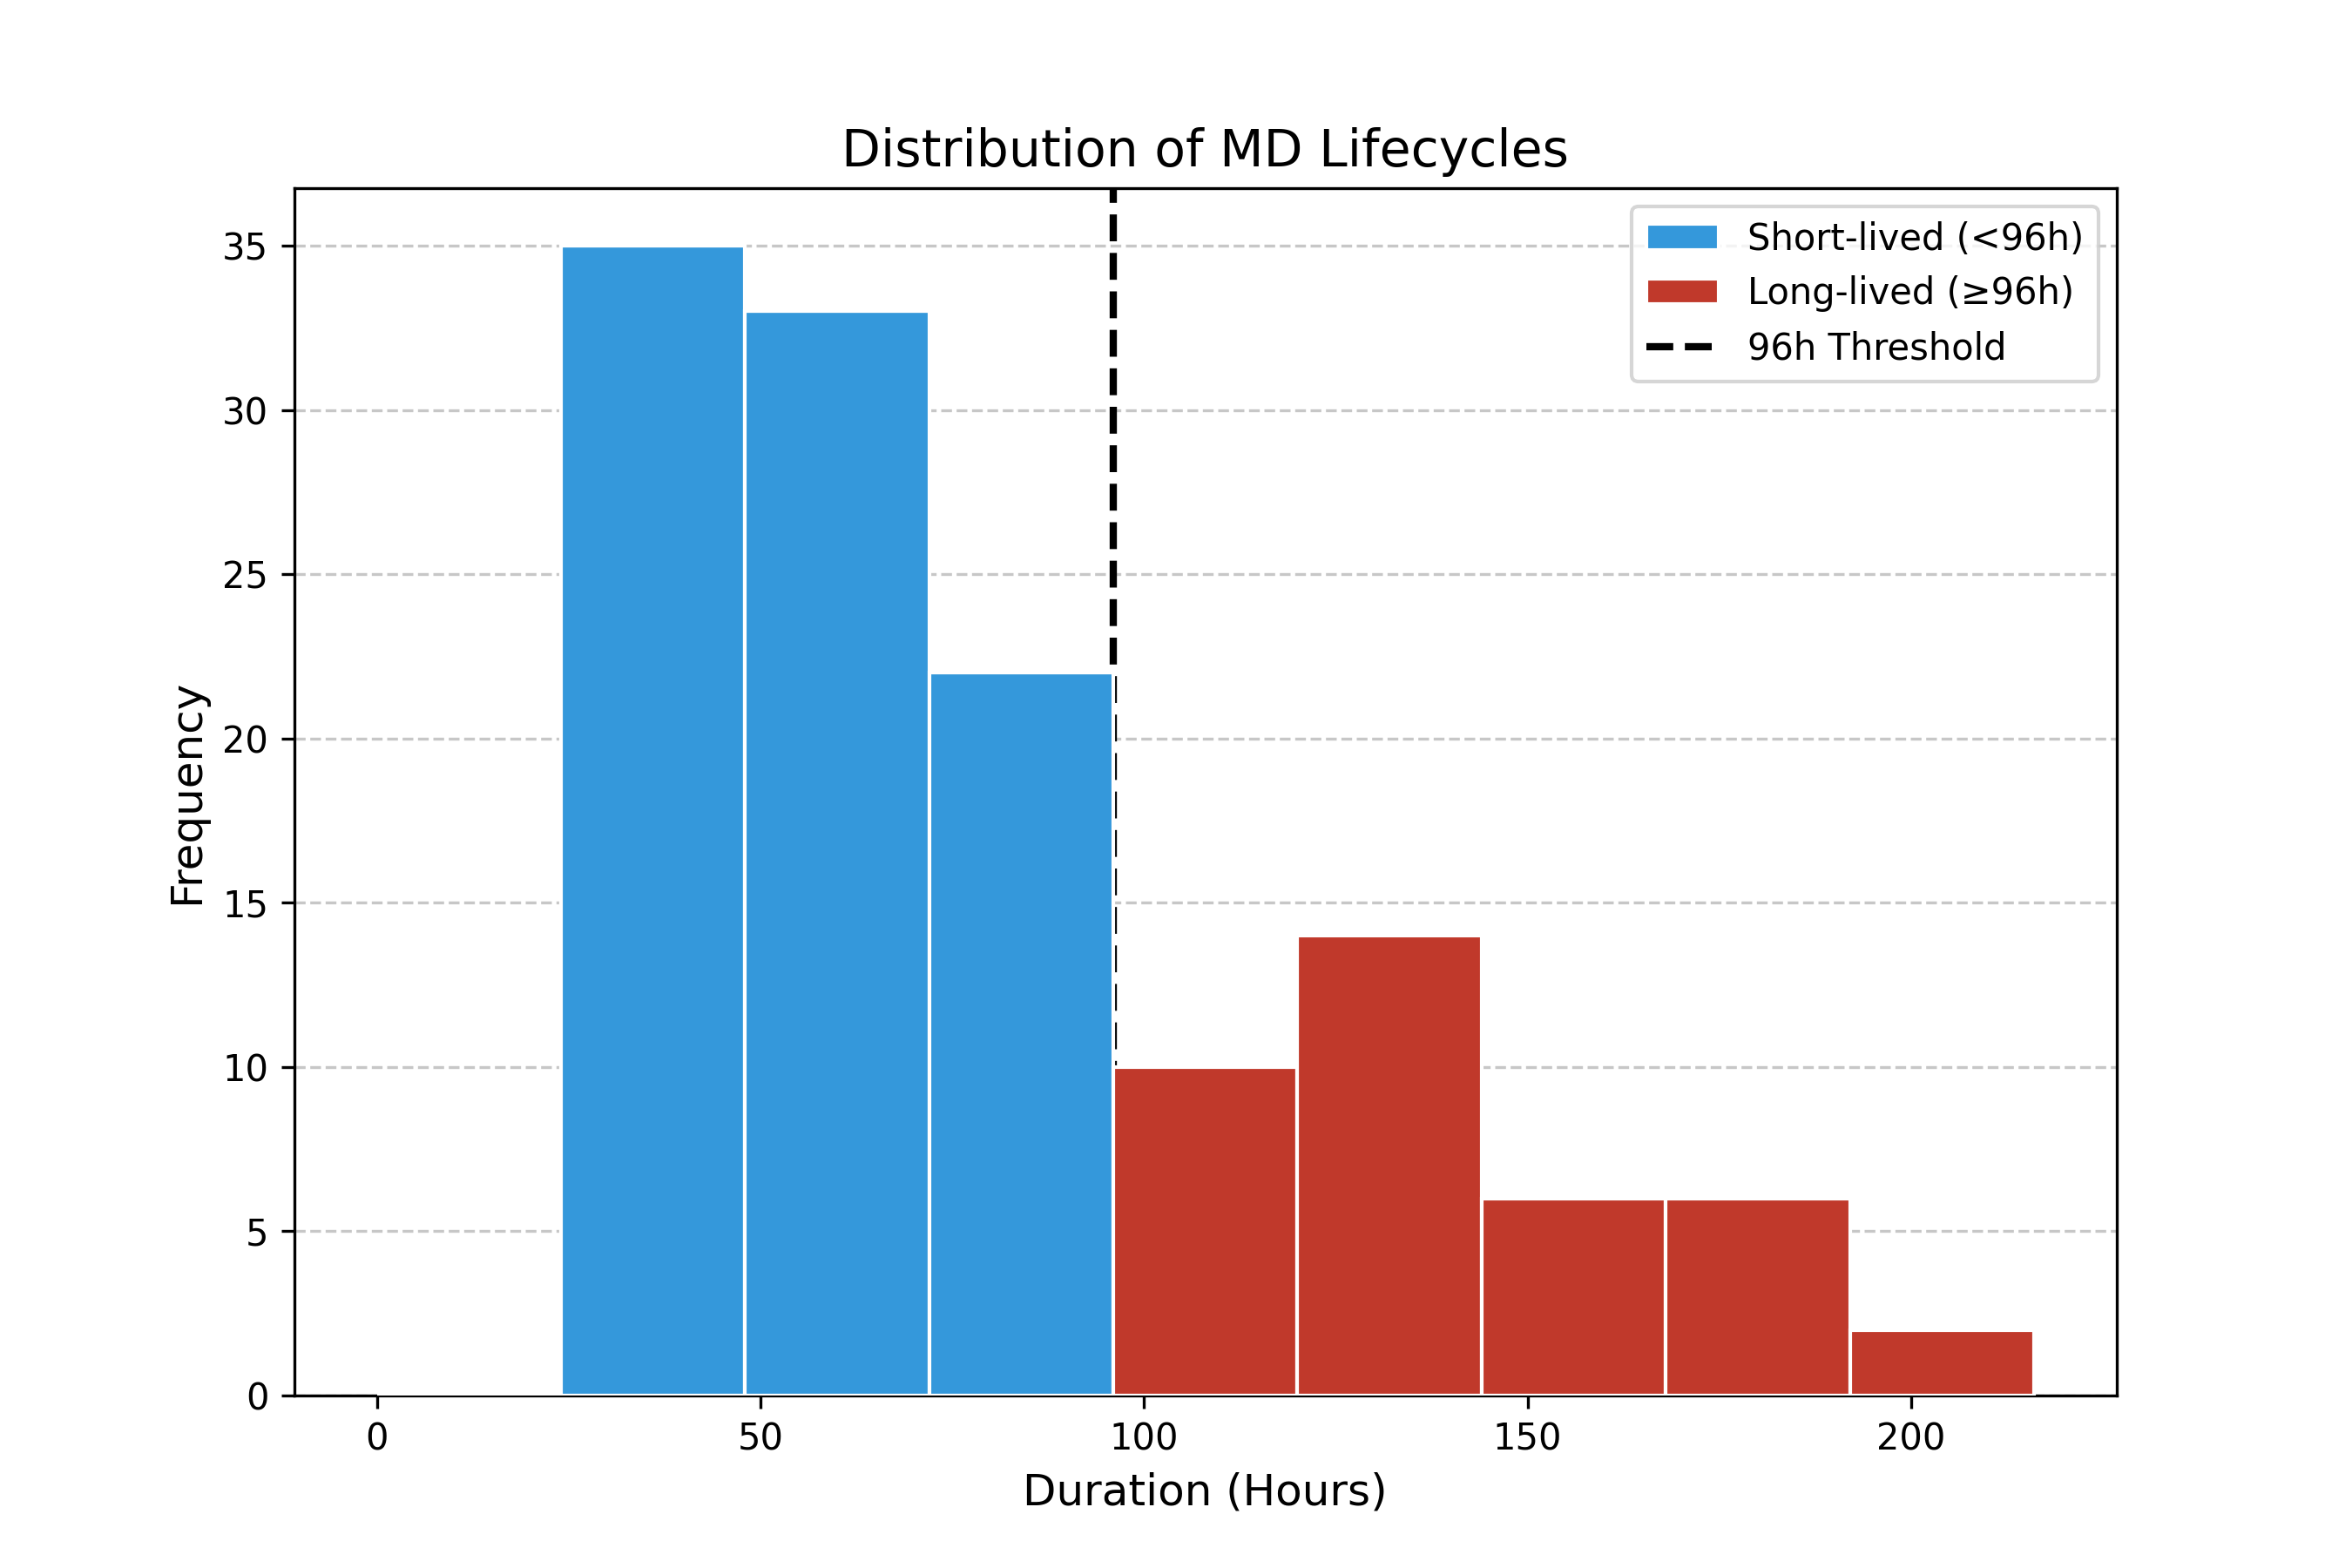
\includegraphics[width=0.80\textwidth]{duration_histogram}
%   \caption[MD duration frequency distribution, 2001-2025]{Frequency
% distribution
%     of MD track durations; dashed line at the 96-hour threshold separates
%   short-lived (blue) and long-lived (red) categories.}
%   \label{fig:duration_histogram}
% \end{figure}
\subsection{2001-2025 Interannual Trends}
\label{subsec:interannual}

Figure~\ref{fig:annual_md_count} presents the annual MD frequency
alongside the count of long-lived systems from 2001 to 2025. Analysis
of this 25-year record reveals two primary signals. First, the total
annual count (averaging $\sim 5.1$ events/year) shows no
statistically significant linear trend ($p > 0.1$), suggesting a
stable the large-scale genesis environment has remained stable,
consistent with \autocite{mishra2021monsoon}.

% Second, the \emph{long-lived fraction} exhibits significant
% interannual variability, ranging from a minimum of \textbf{0.0\%} to
% a maximum of \textbf{66.7\%}. Peak years for long-lived systems,
% specifically \textbf{2016, 2021, and 2024}, coincide with strong
% monsoon seasons where the Gangetic plains and Central India
% exhibited high pre-landfall soil moisture ($> 0.35$\,m$^3$/m$^3$).
% Conversely, during notable deficit years such as \textbf{2001 and 2002},
% the majority of MDs were short-lived, dissipating within 48 hours of
% landfall due to the lack of surface latent heat support from the dry
% antecedent soil.

Second, the number of systems attaining \emph{long-lived status}
(surviving $\geq 96$\,h) shows high interannual variability. In peak
years such as \textbf{2016, 2021, and 2024}, up to 66\% of formed MDs
exhibited extended inland longevity. These years coincide with high
pre-landfall soil moisture ($> 0.35$\,m$^3$/m$^3$). Conversely,
during dry years like 2001, 2002, 2010, 2012 and 2019, zero systems reached
the 96-hour threshold, confirming the surface moisture's role as a
secondary energy source required for inland survival.

\begin{figure}[H]
  \centering
  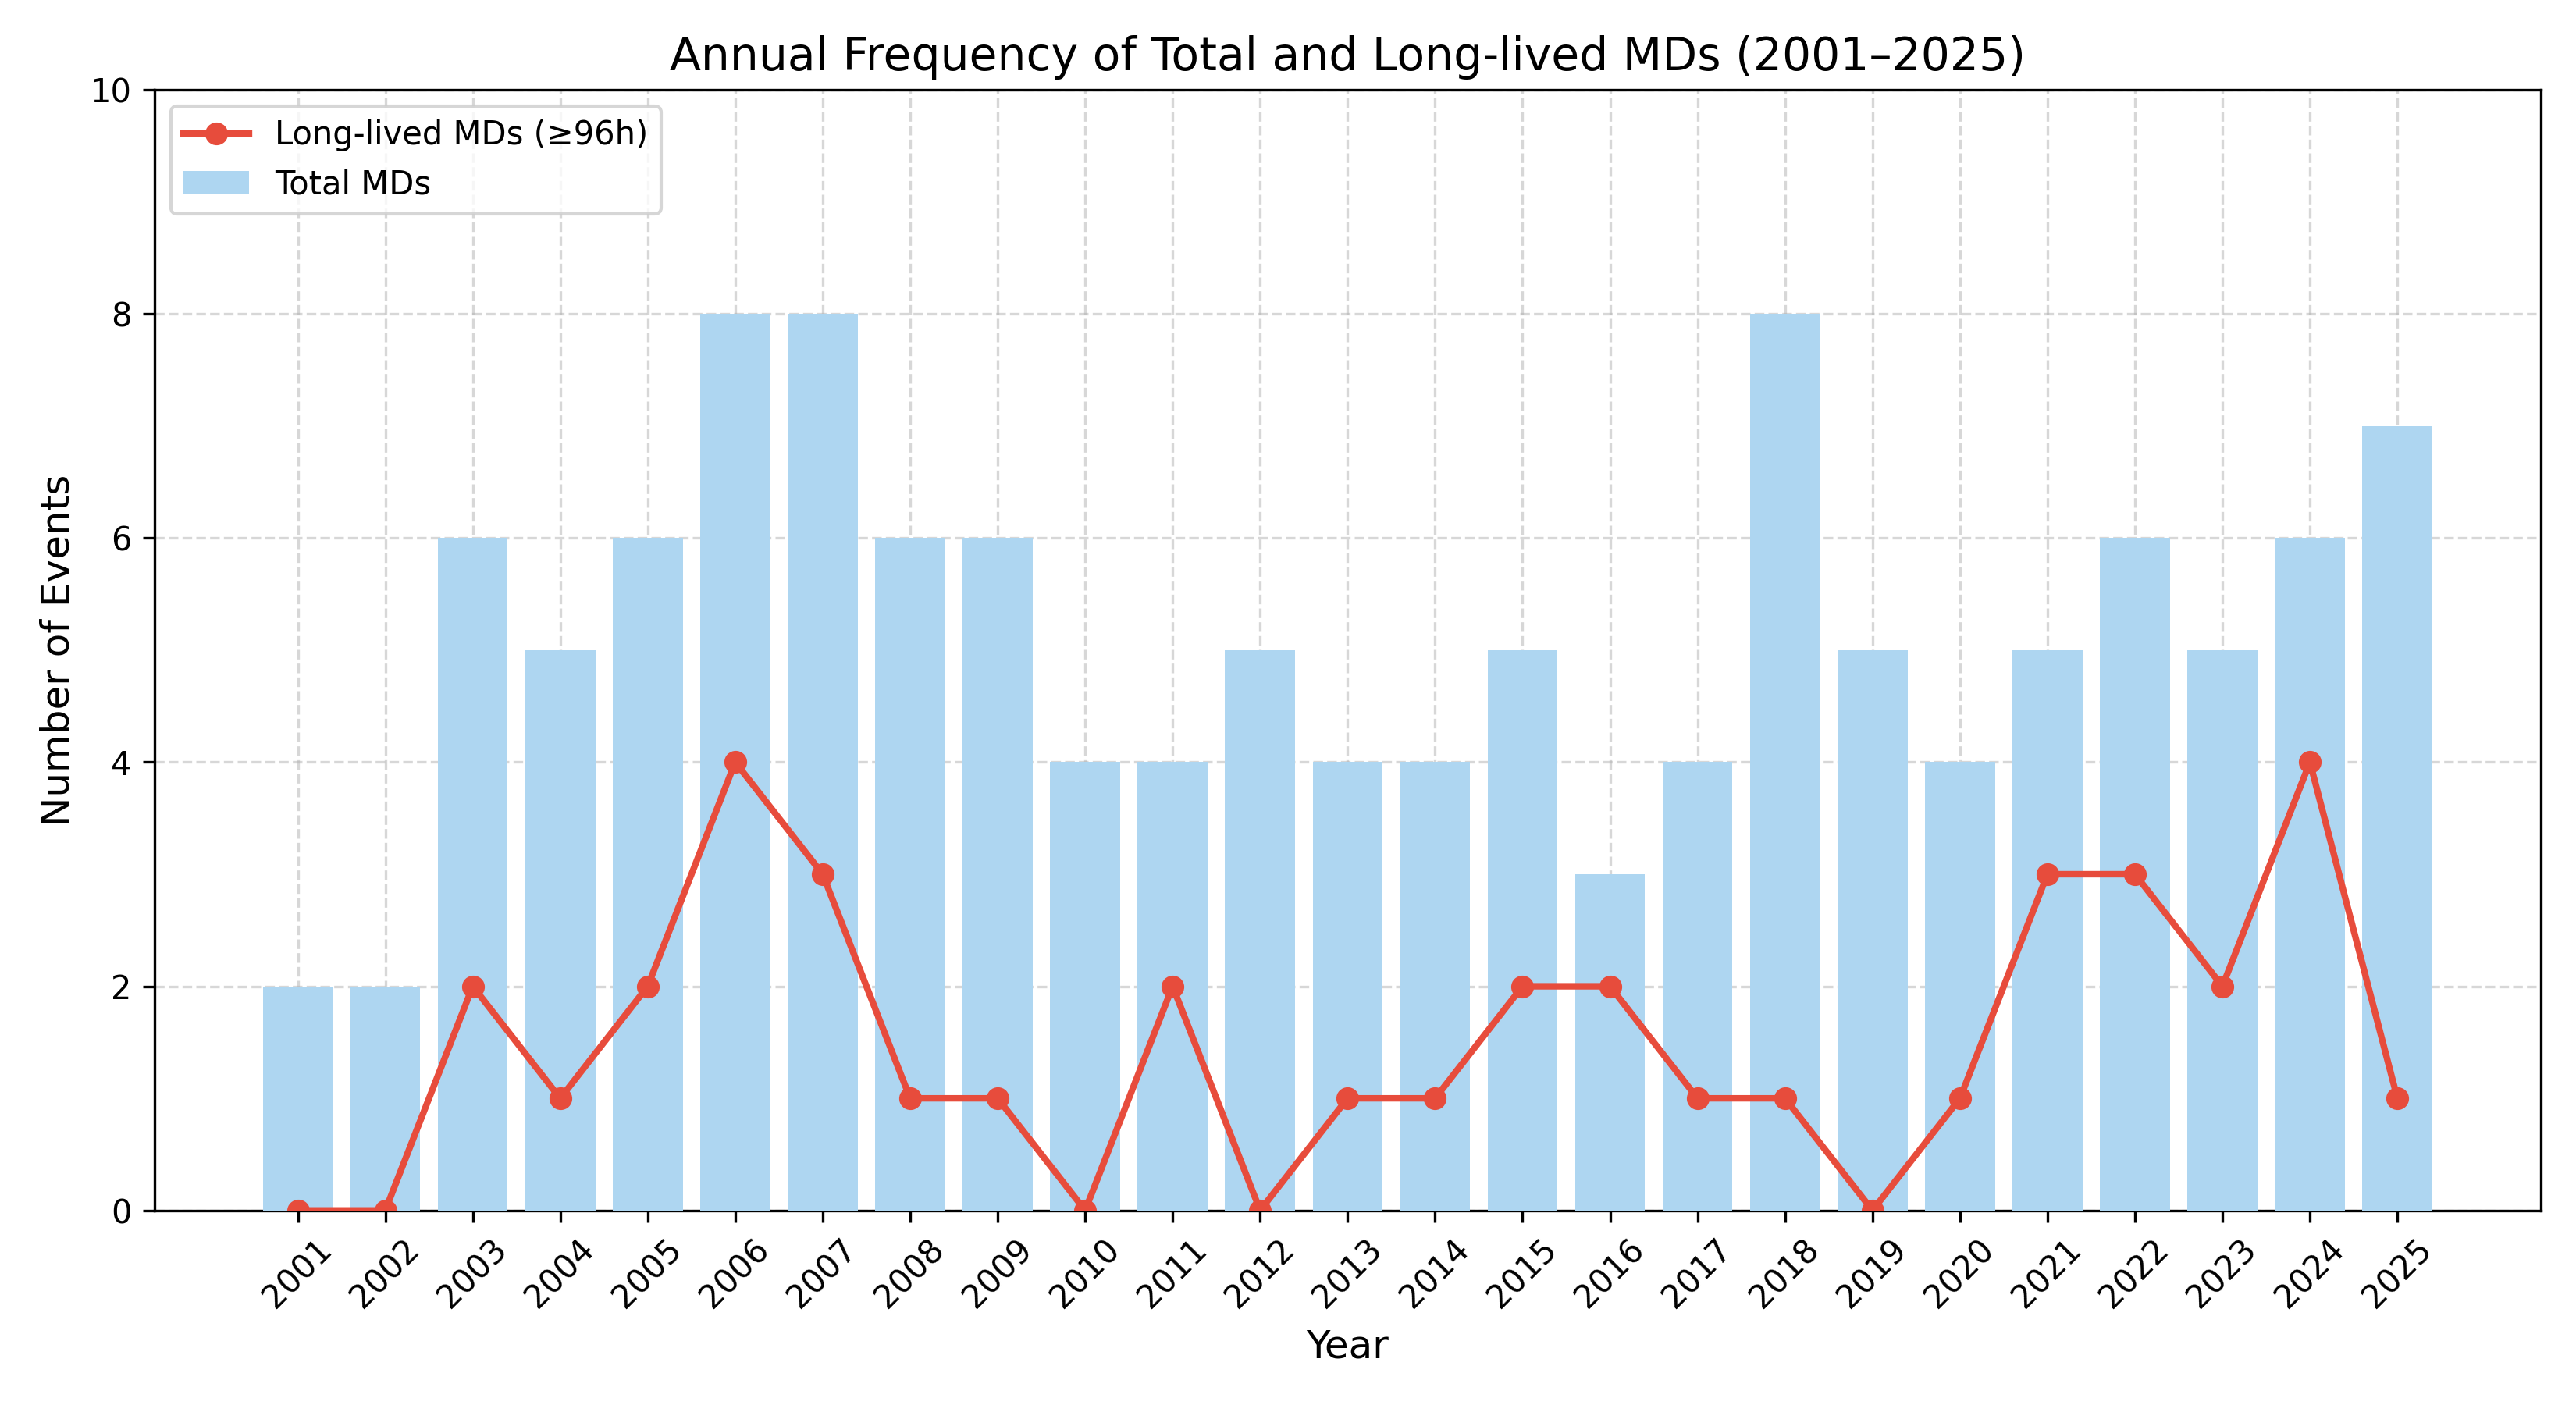
\includegraphics[width=0.86\textwidth]{annual_count_trend}
  \caption[Annual total and long-lived MD counts
  (2001--2025)]{Comparison of total annual MD frequency and the count
    of long-lived systems. The convergence of the line toward the top
  of the bars in years like 2016 indicates high longevity efficiency.}
  \label{fig:annual_md_count}
\end{figure}

The distribution of track durations
(Figure~\ref{fig:duration_histogram}) follows a right-skewed profile.
The ``long-tail'' representing systems surviving $\geq 96$\,h accounts
for approximately \textbf{31\%} of the total population (40 of 128 events).
The fact that this tail does not expand linearly with the total count
suggests that longevity is governed by the state of the land surface
(the BOE) rather than just the frequency of storm genesis.

\begin{figure}[H]
  \centering
  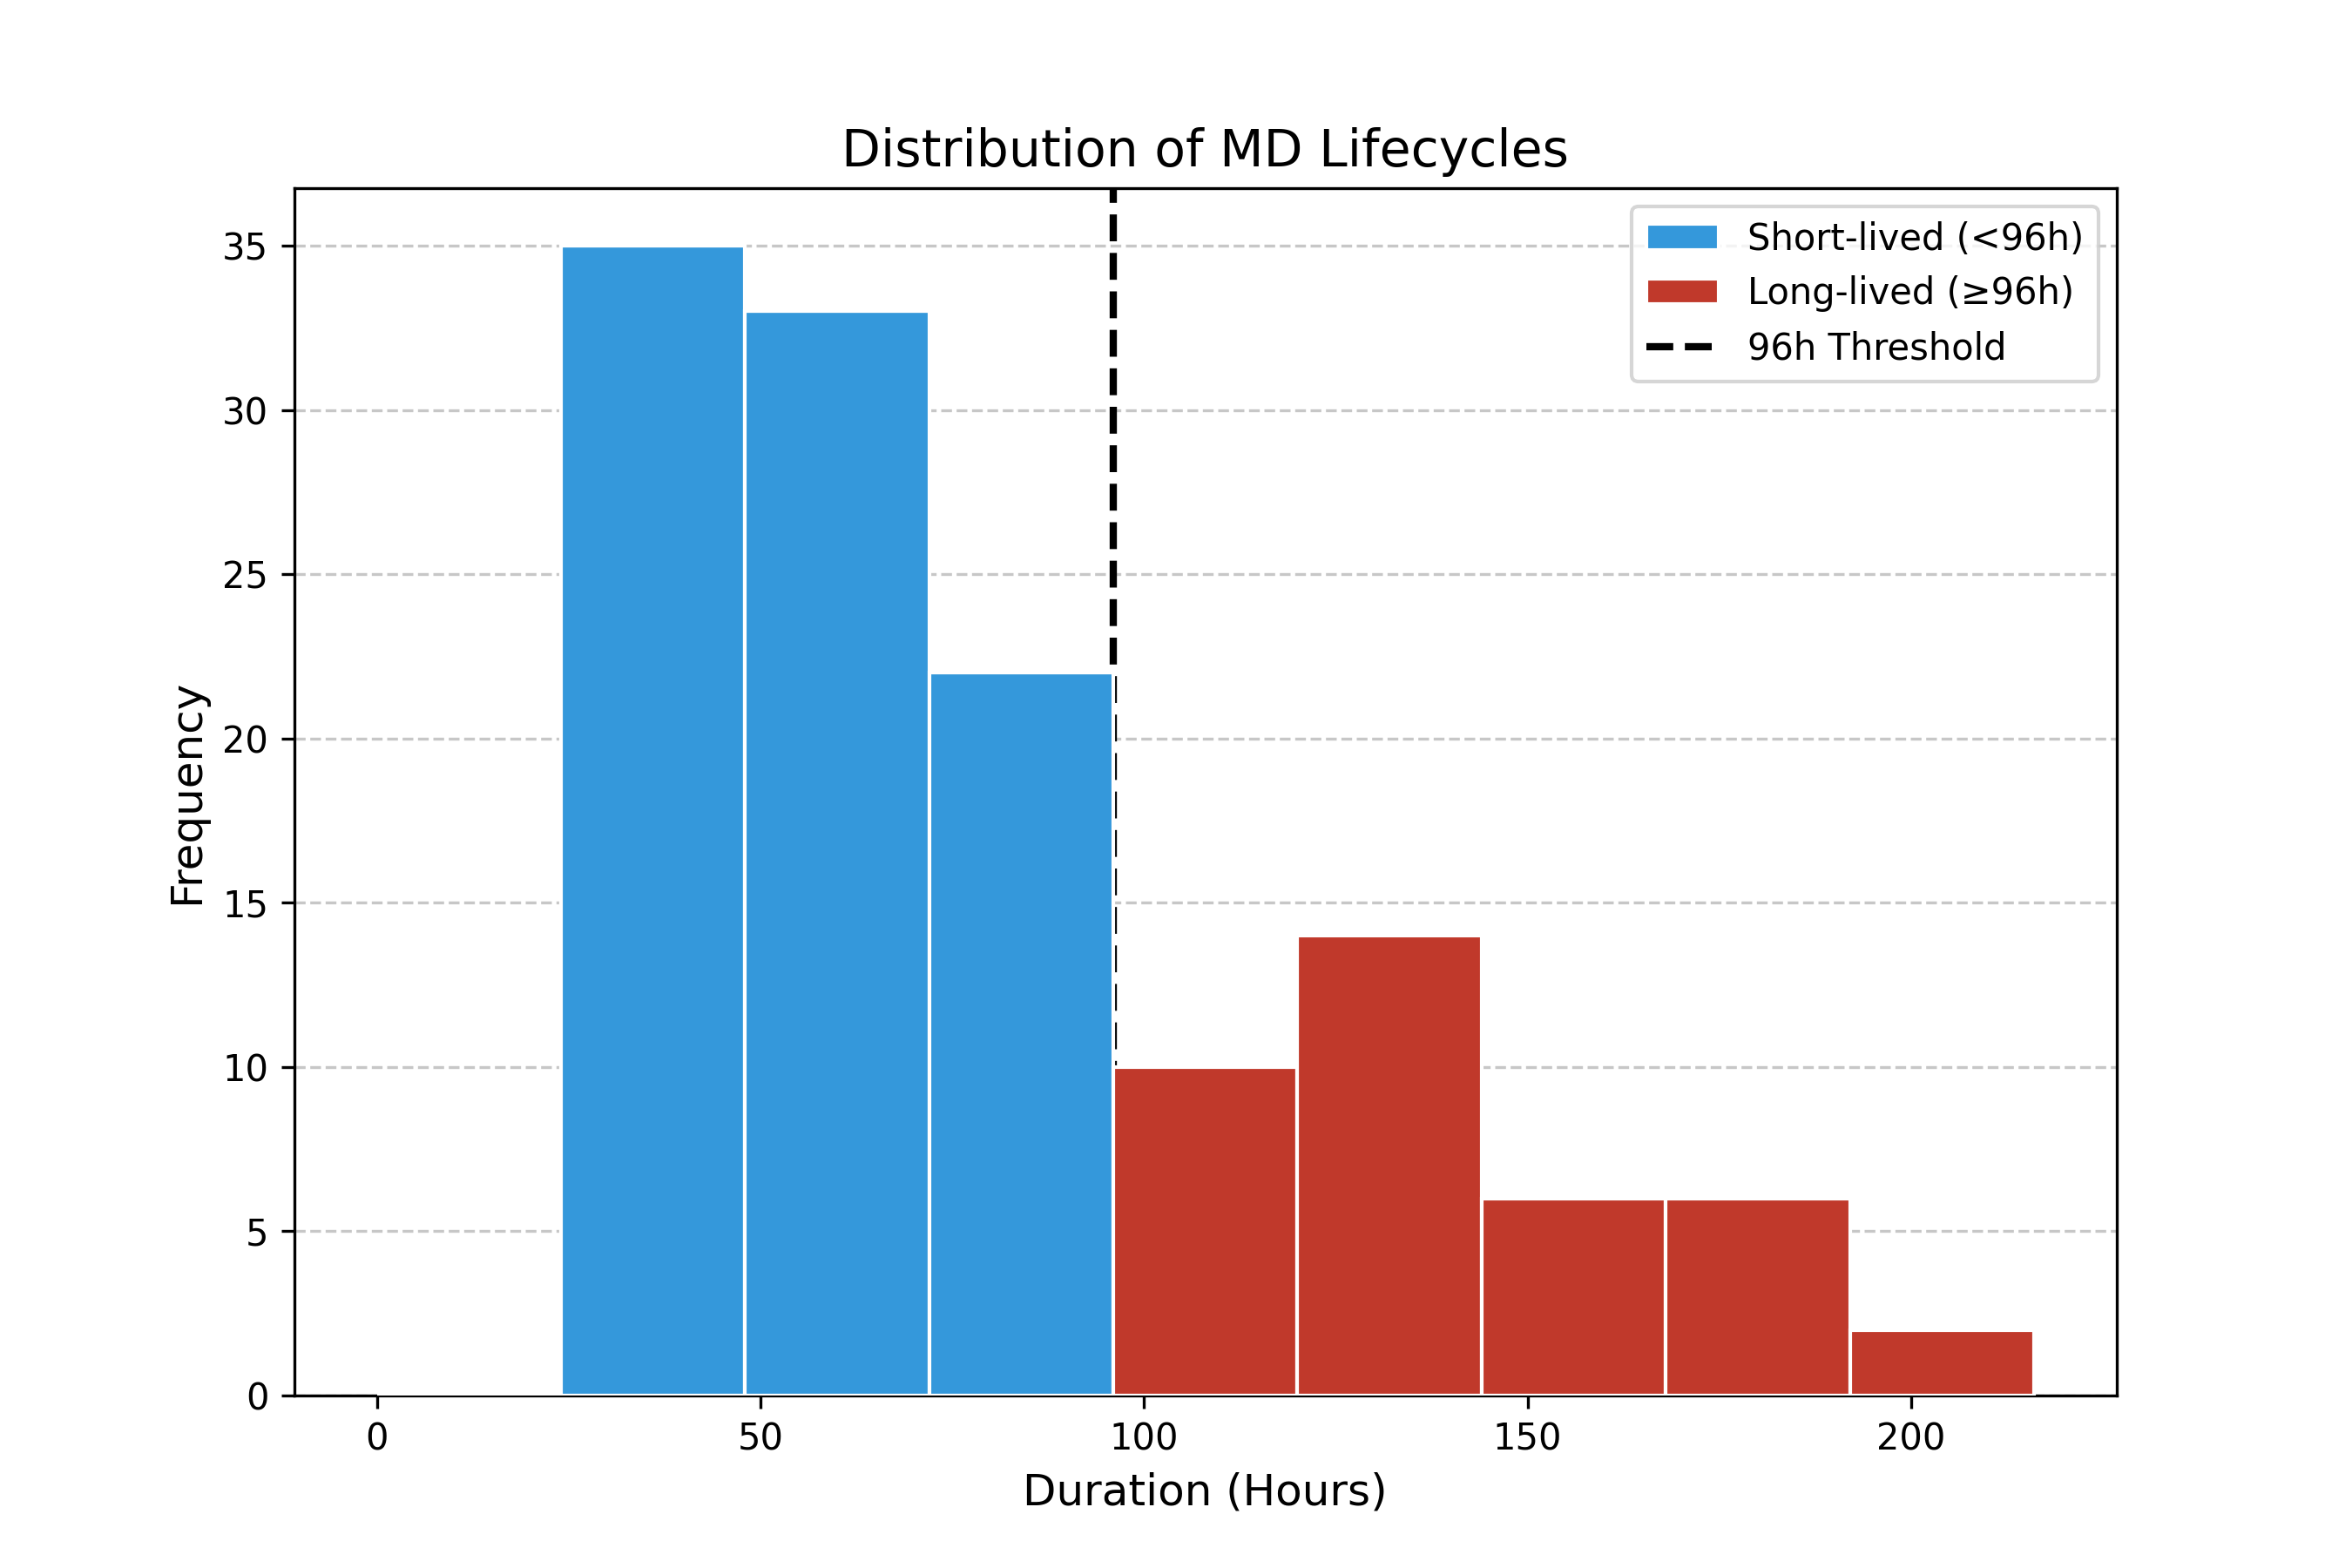
\includegraphics[width=0.75\textwidth]{duration_histogram}
  \caption[MD duration frequency distribution]{Histogram of track
    durations in 24-hour bins. The threshold at 96\,h separates
    short-lived (blue) from long-lived (red) systems, highlighting the
  BOE-sustained population.}
  \label{fig:duration_histogram}
\end{figure}

\subsection{Track Spatial Distribution}
\label{subsec:track_spatial}

Figure~\ref{fig:all_years_track_elevation} shows short-lived systems
predominantly terminate within 200--400\,km of the coastline, east of
the Eastern Ghats 600\,m contour. This spatial clustering is
consistent with terrain-induced structural disruption preventing
further inland transit in systems without an adequate surface energy
source. Long-lived systems extend well west of the Ghats into the
Gangetic plain, Madhya Pradesh and Maharasthra, indicating successful
terrain traversal. The spatial clustering of long-lived tracks over
the Gangetic plain corresponds closely to the region of highest
climatological July-August \texttt{swvl1} ($>0.3$\,m$^3$\,m$^{-3}$),
broadly consistent with the BOE hypothesis.

\textbf{Ocean-originated vs. land-genesis tracks :} Of the
\textbf{128} total events, \textbf{96.8\%} (124 events) originated
over the Bay of Bengal and made landfall along the eastern coast,
while only \textbf{3.2\%} (4 Land MDs) formed over the land surface
directly. This highlights that the vast majority of the MD population
relies on an initial oceanic moisture supply. Ocean-originated tracks
show a distinctly different thermodynamic evolution: they arrive at
the coast with well-organised vorticity, a sustained outer rainband,
and inner-core LHF of 100-150\,W\,m$^{-2}$ built up over 1-3 days
of oceanic energy supply.

This strong energetic initial condition means that even moderately
moist antecedent soils ($\texttt{swvl1} \approx 0.28$--$0.32$
\,m$^3$\,m$^{-3}$) may be sufficient to sustain the BOE in these
systems, since the MD arrives at the coast in a more intensified
state and the transition timescale to land-phase dependence is
longer. Land-originated systems, lacking this oceanic spin-up phase,
tend to be shorter-lived unless they form over a region of
anomalously high soil moisture.

\begin{figure}[H]
  \centering
  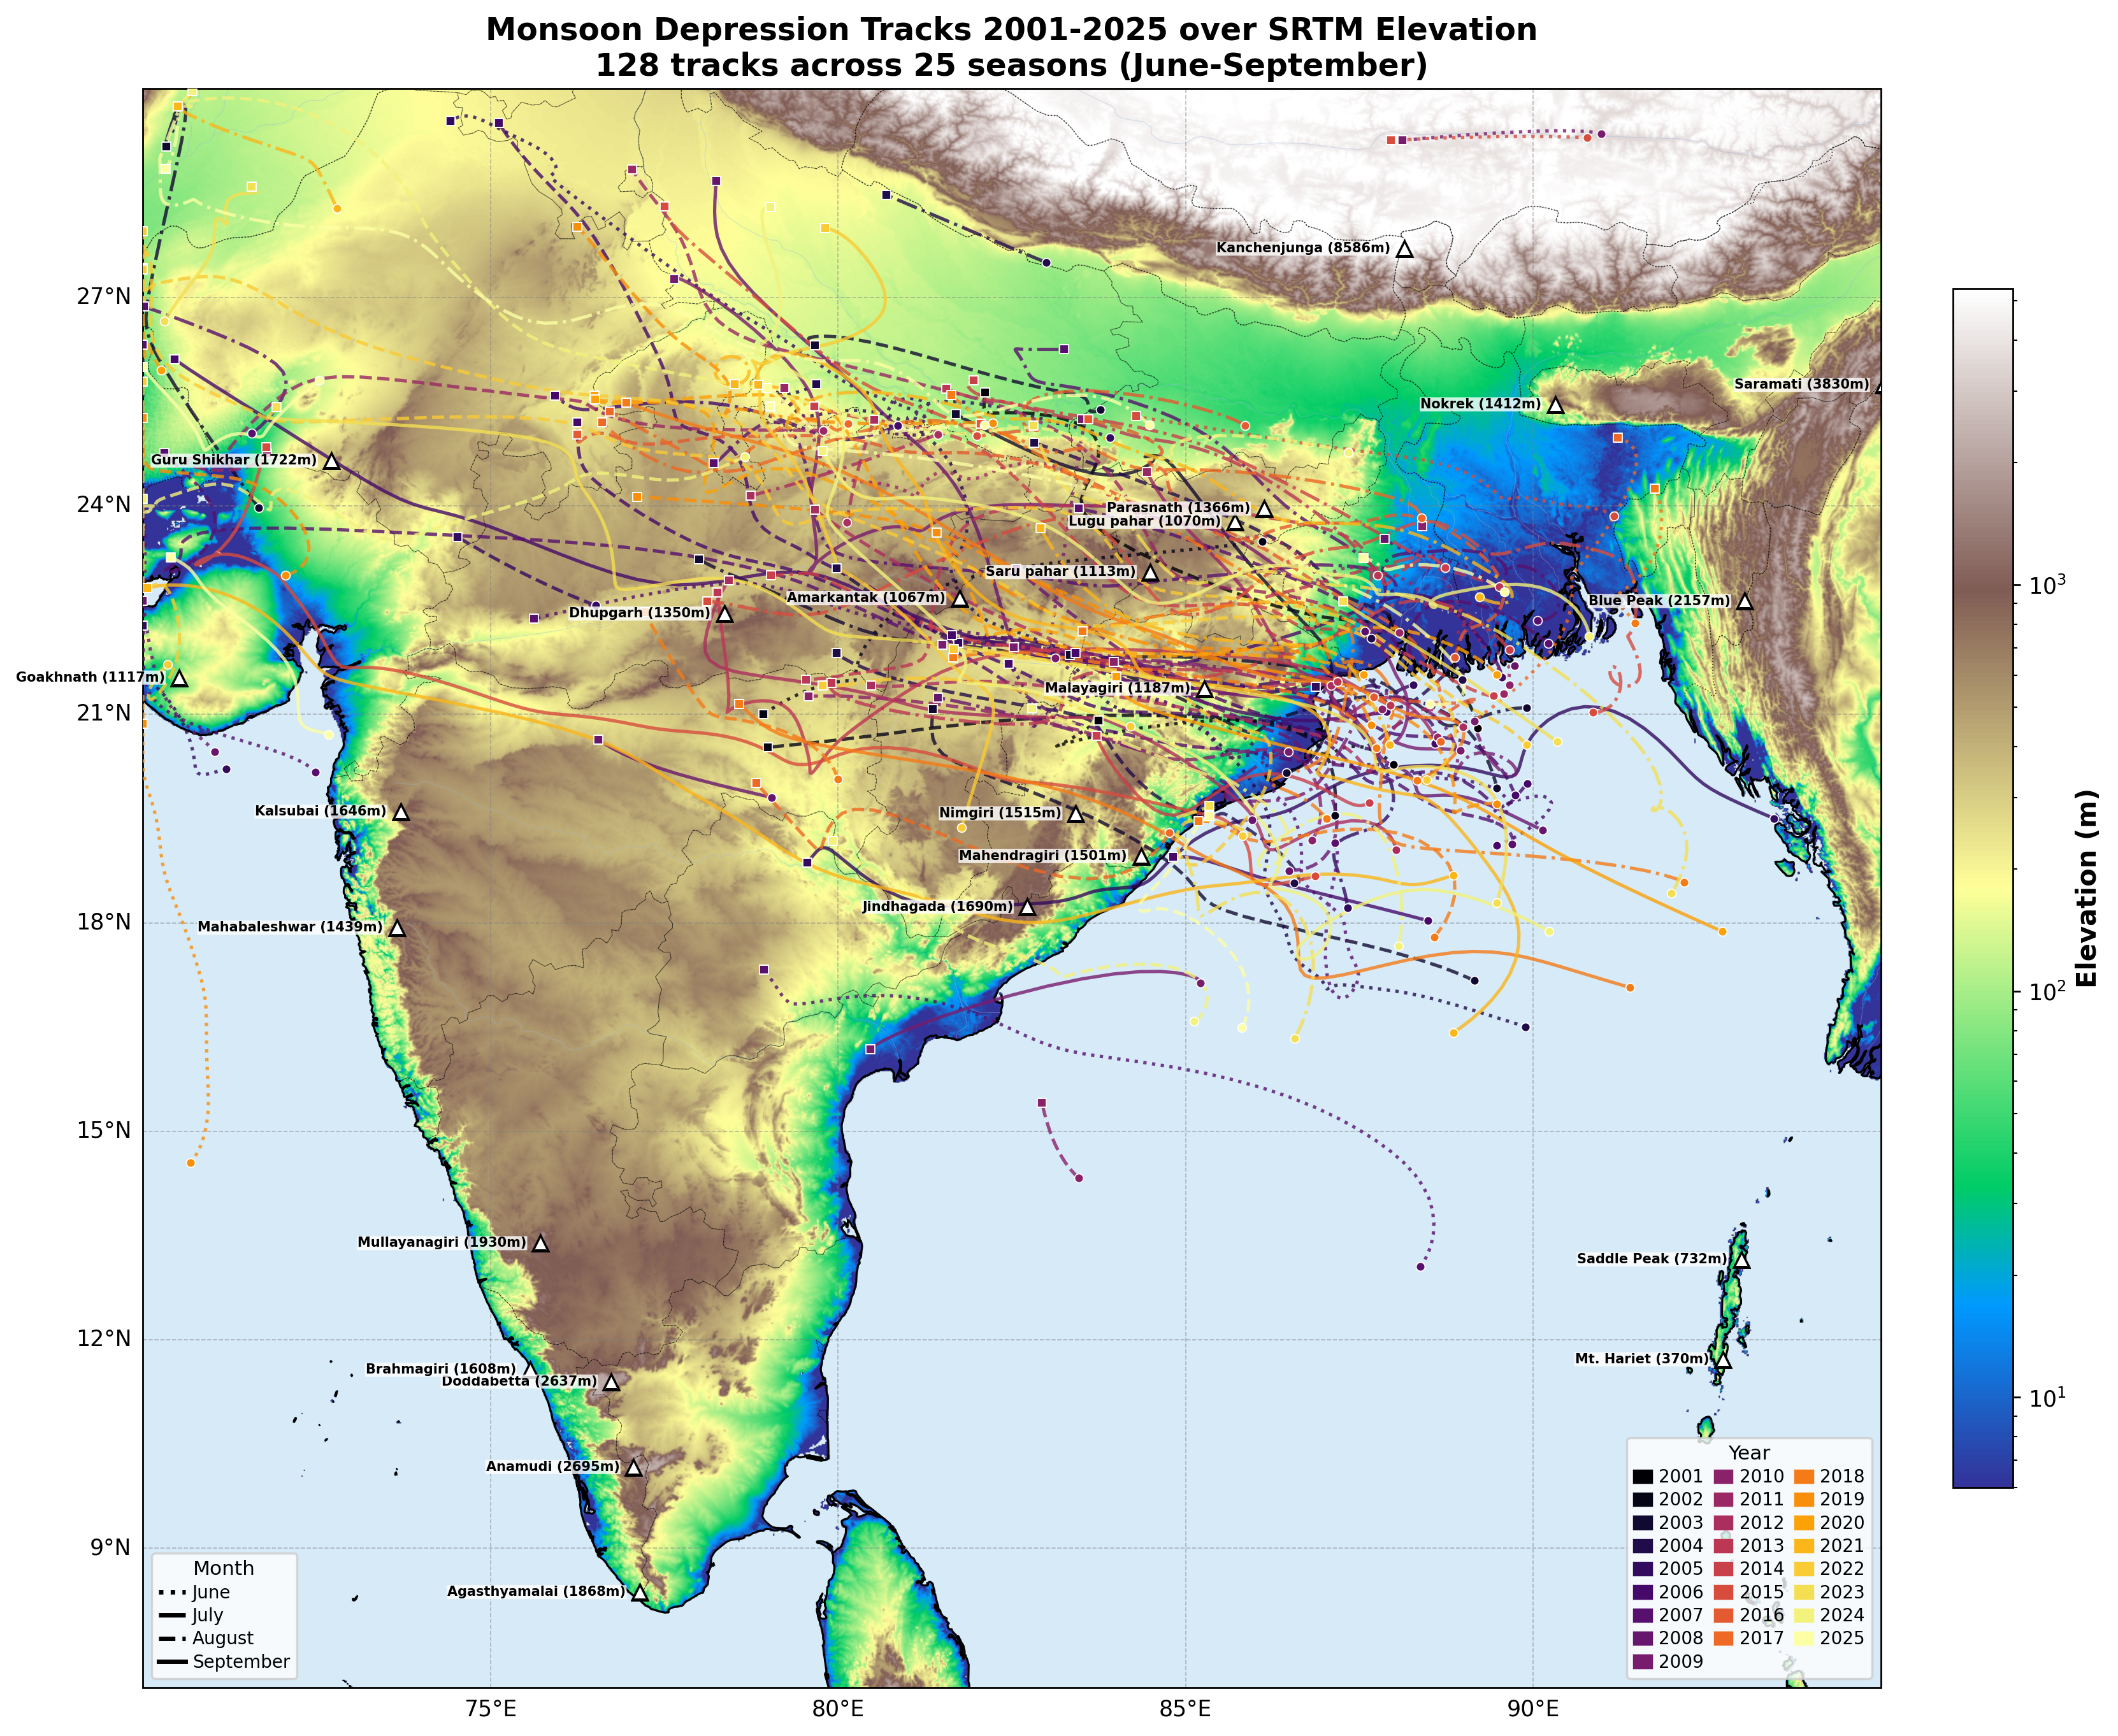
\includegraphics[width=0.92\textwidth]{all_years_tracks_elevation.png}
  \caption[Spatial distribution of MD tracks by duration
  category]{All confirmed MD tracks (2001--2025) coloured by
    duration; Eastern Ghats 600\,m contour overlaid. Landfall points
    marked by filled circles. Long-lived tracks cluster over the
  Gangetic plain west of the terrain.}
  \label{fig:all_years_track_elevation}
\end{figure}

% %%  FIGURE: All-track spatial map
% %%  SOURCE: Overall_years/MD_all_tracks_coloured_duration.png
% %%  Colour tracks by duration bins; add 600m Eastern Ghats contour;
% % mark landfall points.
% %%  Also overlay ERA5 July-August SWVL1 climatology as background
% % shading (optional).
% \begin{figure}[H]
%   \centering
%   \fbox{\rule{0pt}{7cm}\rule{0.90\textwidth}{0pt}}
%   % \includegraphics[width=0.90\textwidth]{all_md_tracks_coloured}
%   \caption[Spatial distribution of MD tracks by duration
%   category]{All confirmed MD tracks (2001-2025) coloured by
% duration; Eastern Ghats 600\,m contour (bold grey) overlaid.
% Landfall points marked by filled circles. Long-lived tracks cluster
% over the Gangetic plain west of the terrain.}
%   \label{fig:all_md_tracks_results}
% \end{figure}

\subsection{Annual MD Count and BOE Frequency}
\label{subsec:multiyear_count}

% Figure~\ref{fig:annual_md_count_boe_fraction} displays the annual
% frequency of MDs alongside the fraction of systems meeting the BOE
% candidacy criteria ($\geq 70$,W,m$^{-2}$ LHF for $\geq 18$,h).

Two primary observations emerge from the climatology:
\begin{enumerate}
  \item \textbf{Stability of Genesis:} The total annual MD count
    shows no statistically significant monotonic trend ($p > 0.1$),
    consistent with the findings of \autocite{mishra2021monsoon}
    regarding stable synoptic frequency.
  \item \textbf{BOE Variability:} The BOE candidate fraction is
    substantially more variable year-to-year than the total count.
    This demonstrates that post-landfall persistence is not a simple
    function of genesis frequency, but is controlled by a state
    variable-land-surface moisture-that fluctuates independently of
    the large-scale atmospheric triggers for genesis.
\end{enumerate}

% \begin{figure}[H]
%   \centering
%   \includegraphics[width=0.88\textwidth]{Overall_years/annual_md_count_boe_fraction}
%   \caption{Annual MD count and BOE-candidate fraction over
%     2001--2025. The high interannual variability of the BOE fraction
%   suggests land-surface control over system longevity.}
%   \label{fig:annual_md_count_boe_fraction}
% \end{figure}

% \section{Azimuthal Hovm\"{o}ller Analysis}
\section{Azimuthal Hovm\texorpdfstring{\"{o}}{o}ller Analysis}
\label{sec:results_hovmoller}

While the climatological overview established the frequency of inland
penetration, this section identifies the physical mechanisms governing
that sustainability through an azimuthal perspective. By transforming the
MD into a storm-centered radial coordinate system, we can isolate the
evolution of the inner-core thermodynamics, where the BOE feedback is most
important, from the surrounding large-scale monsoon flow. Therefore we
identify the radial-temporal signature of the BOE by comparing the evolution
of long-lived (BOE-active) and short-lived (Non-BOE) MDs across the 2001–2025
period that govern inland sustainability. % By centering the analysis on
% landfall ($t=0$), we isolate the transition from oceanic to terrestrial
% energy dependence.

The analysis is centered on the moment of landfall ($t=0$) to capture
the critical transition from oceanic to terrestrial energy
dependence. To contrast the differing regimes, we examine two
representative cases from the 2001–2025 database:
\begin{itemize}
  \item \textbf{BOE-Active (Long-lived):} Track 5 from September 2024
    (6th to 12th September), which successfully navigated the Eastern
    Ghats and penetrated deep into the Indian heartland.
  \item \textbf{Non-BOE (Short-lived):} A June 2001 system (11th to
    14th June) that underwent rapid structural collapse shortly after landfall.
\end{itemize}

% --- BOE-ACTIVE SYSTEM ---
\begin{figure}[H]
  \centering
  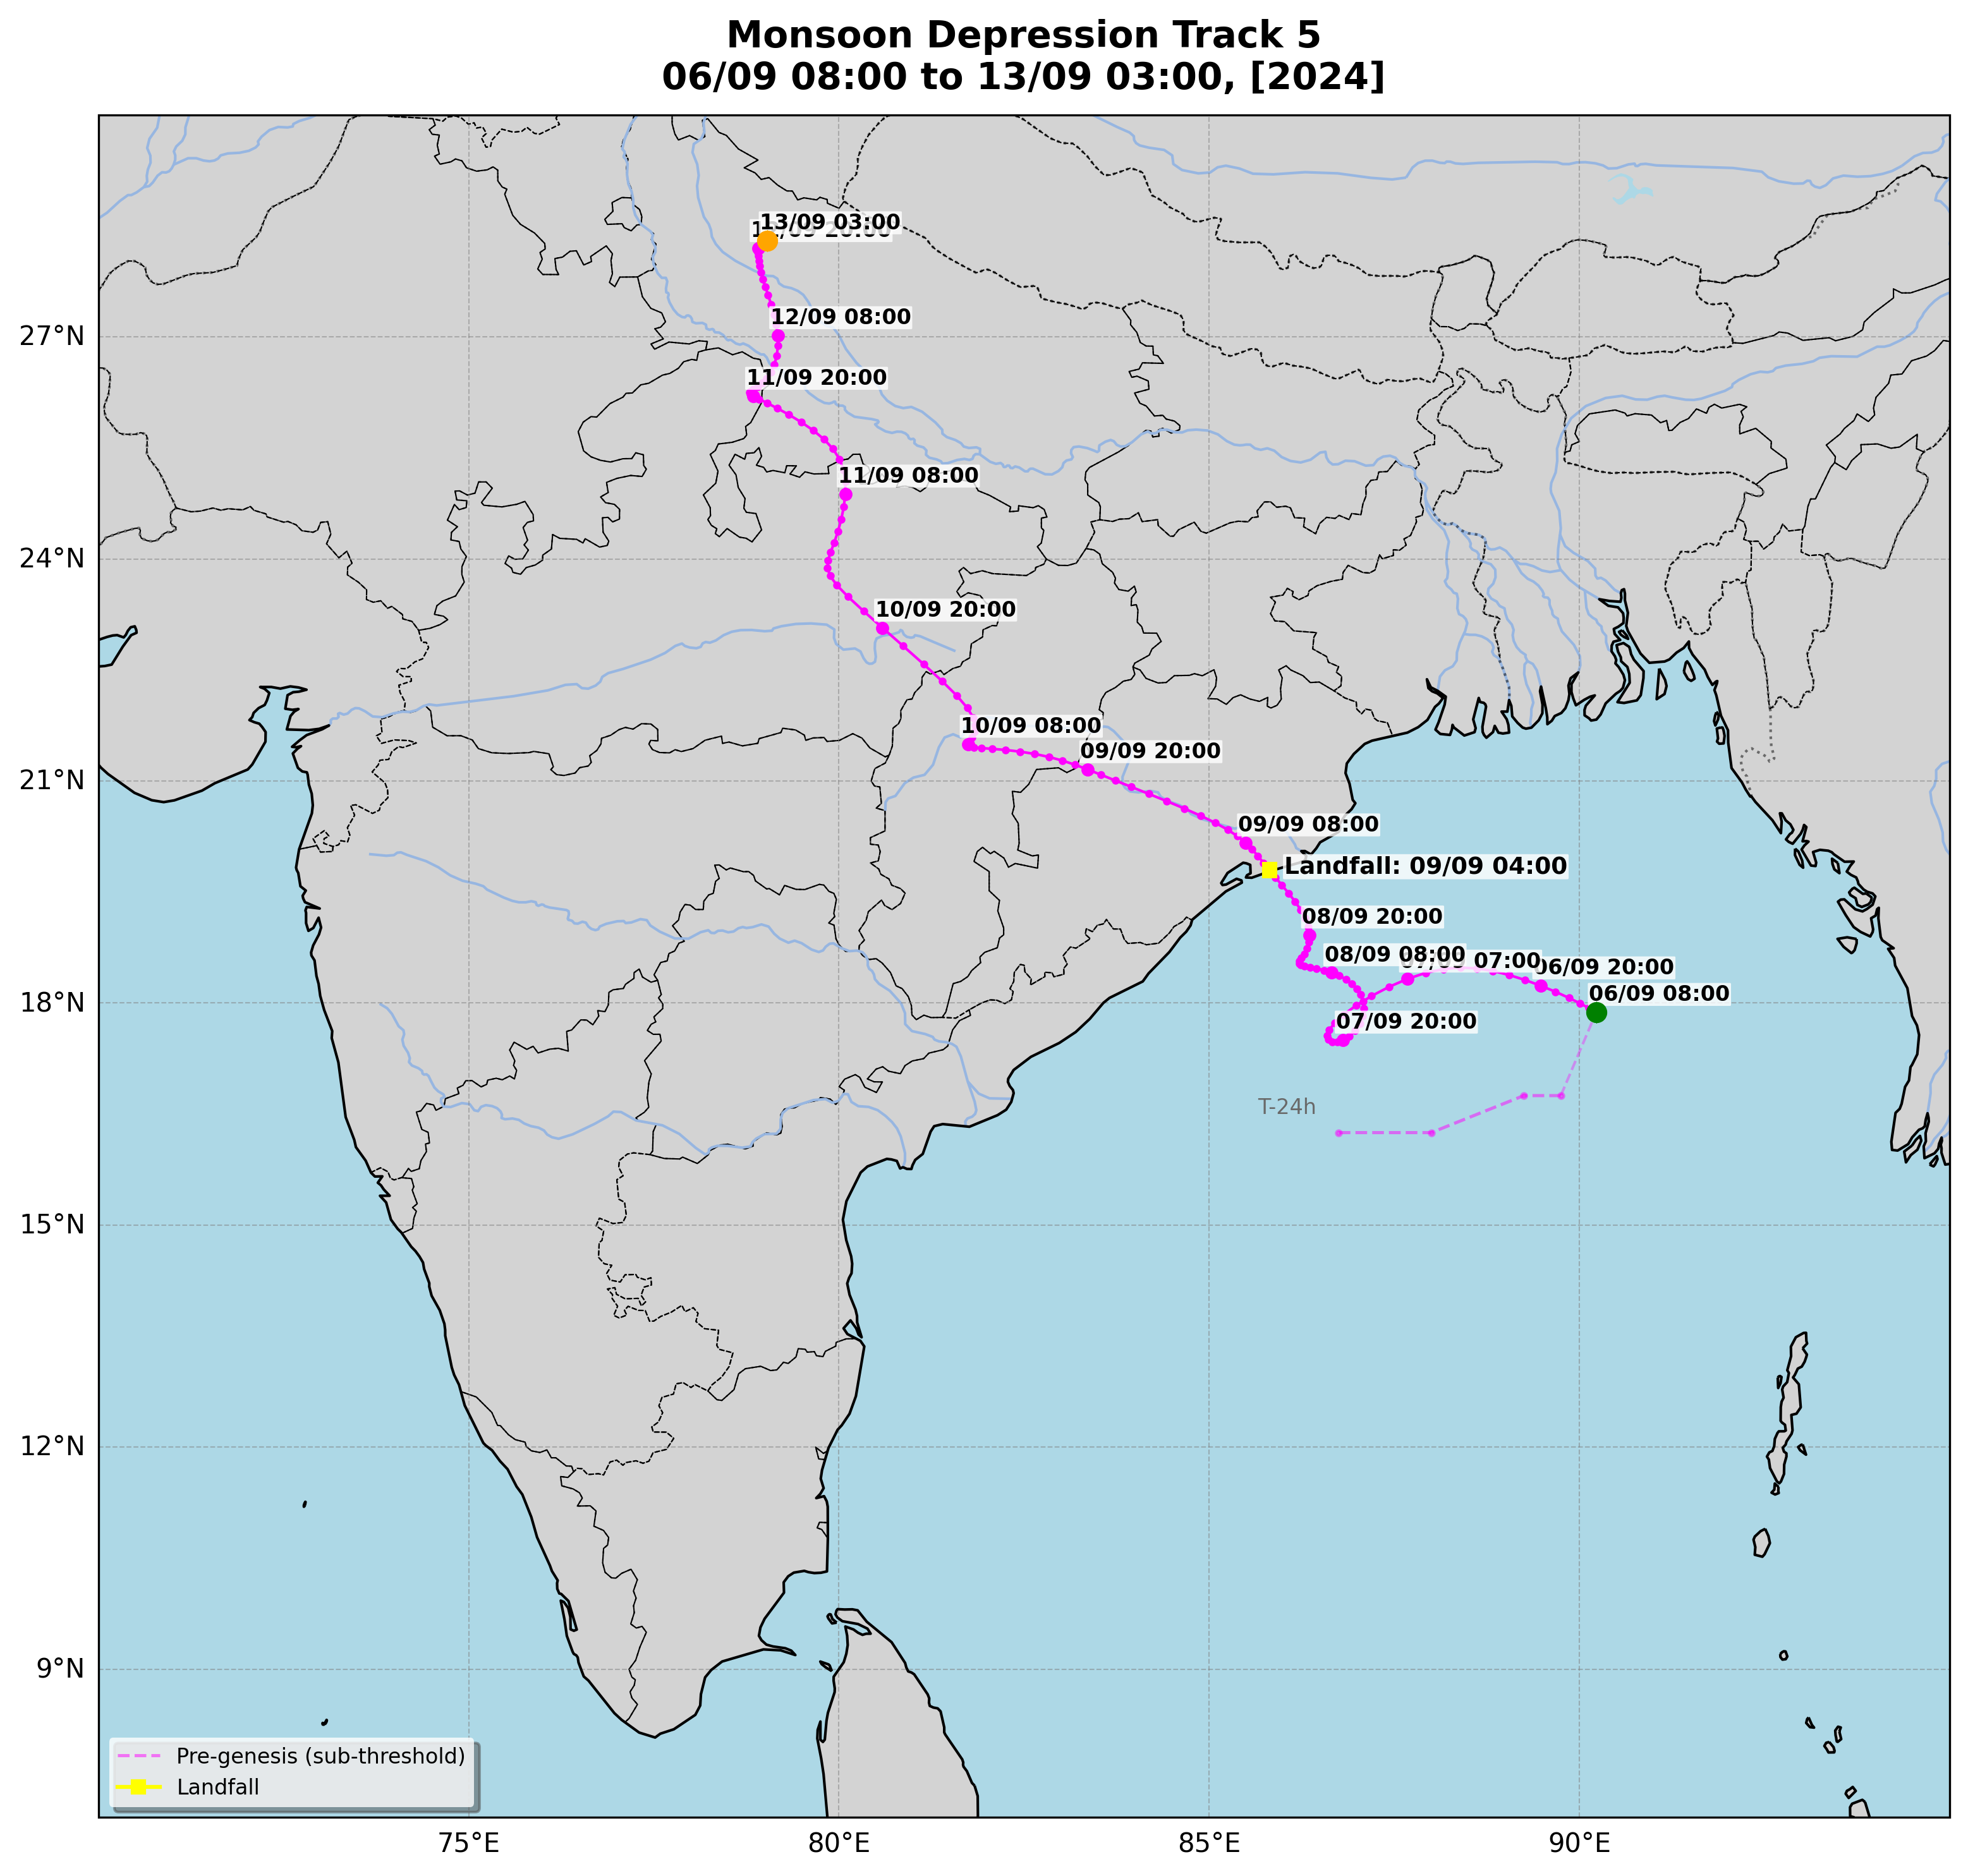
\includegraphics[width=0.67\textwidth]{track_long_spatial}
  \caption{Long-lived Track (Sept 2024), BOE Track Path}
  \label{fig:tp_long_spatial}
\end{figure}

% --- NON-BOE SYSTEM ---
\begin{figure}[H]
  \centering
  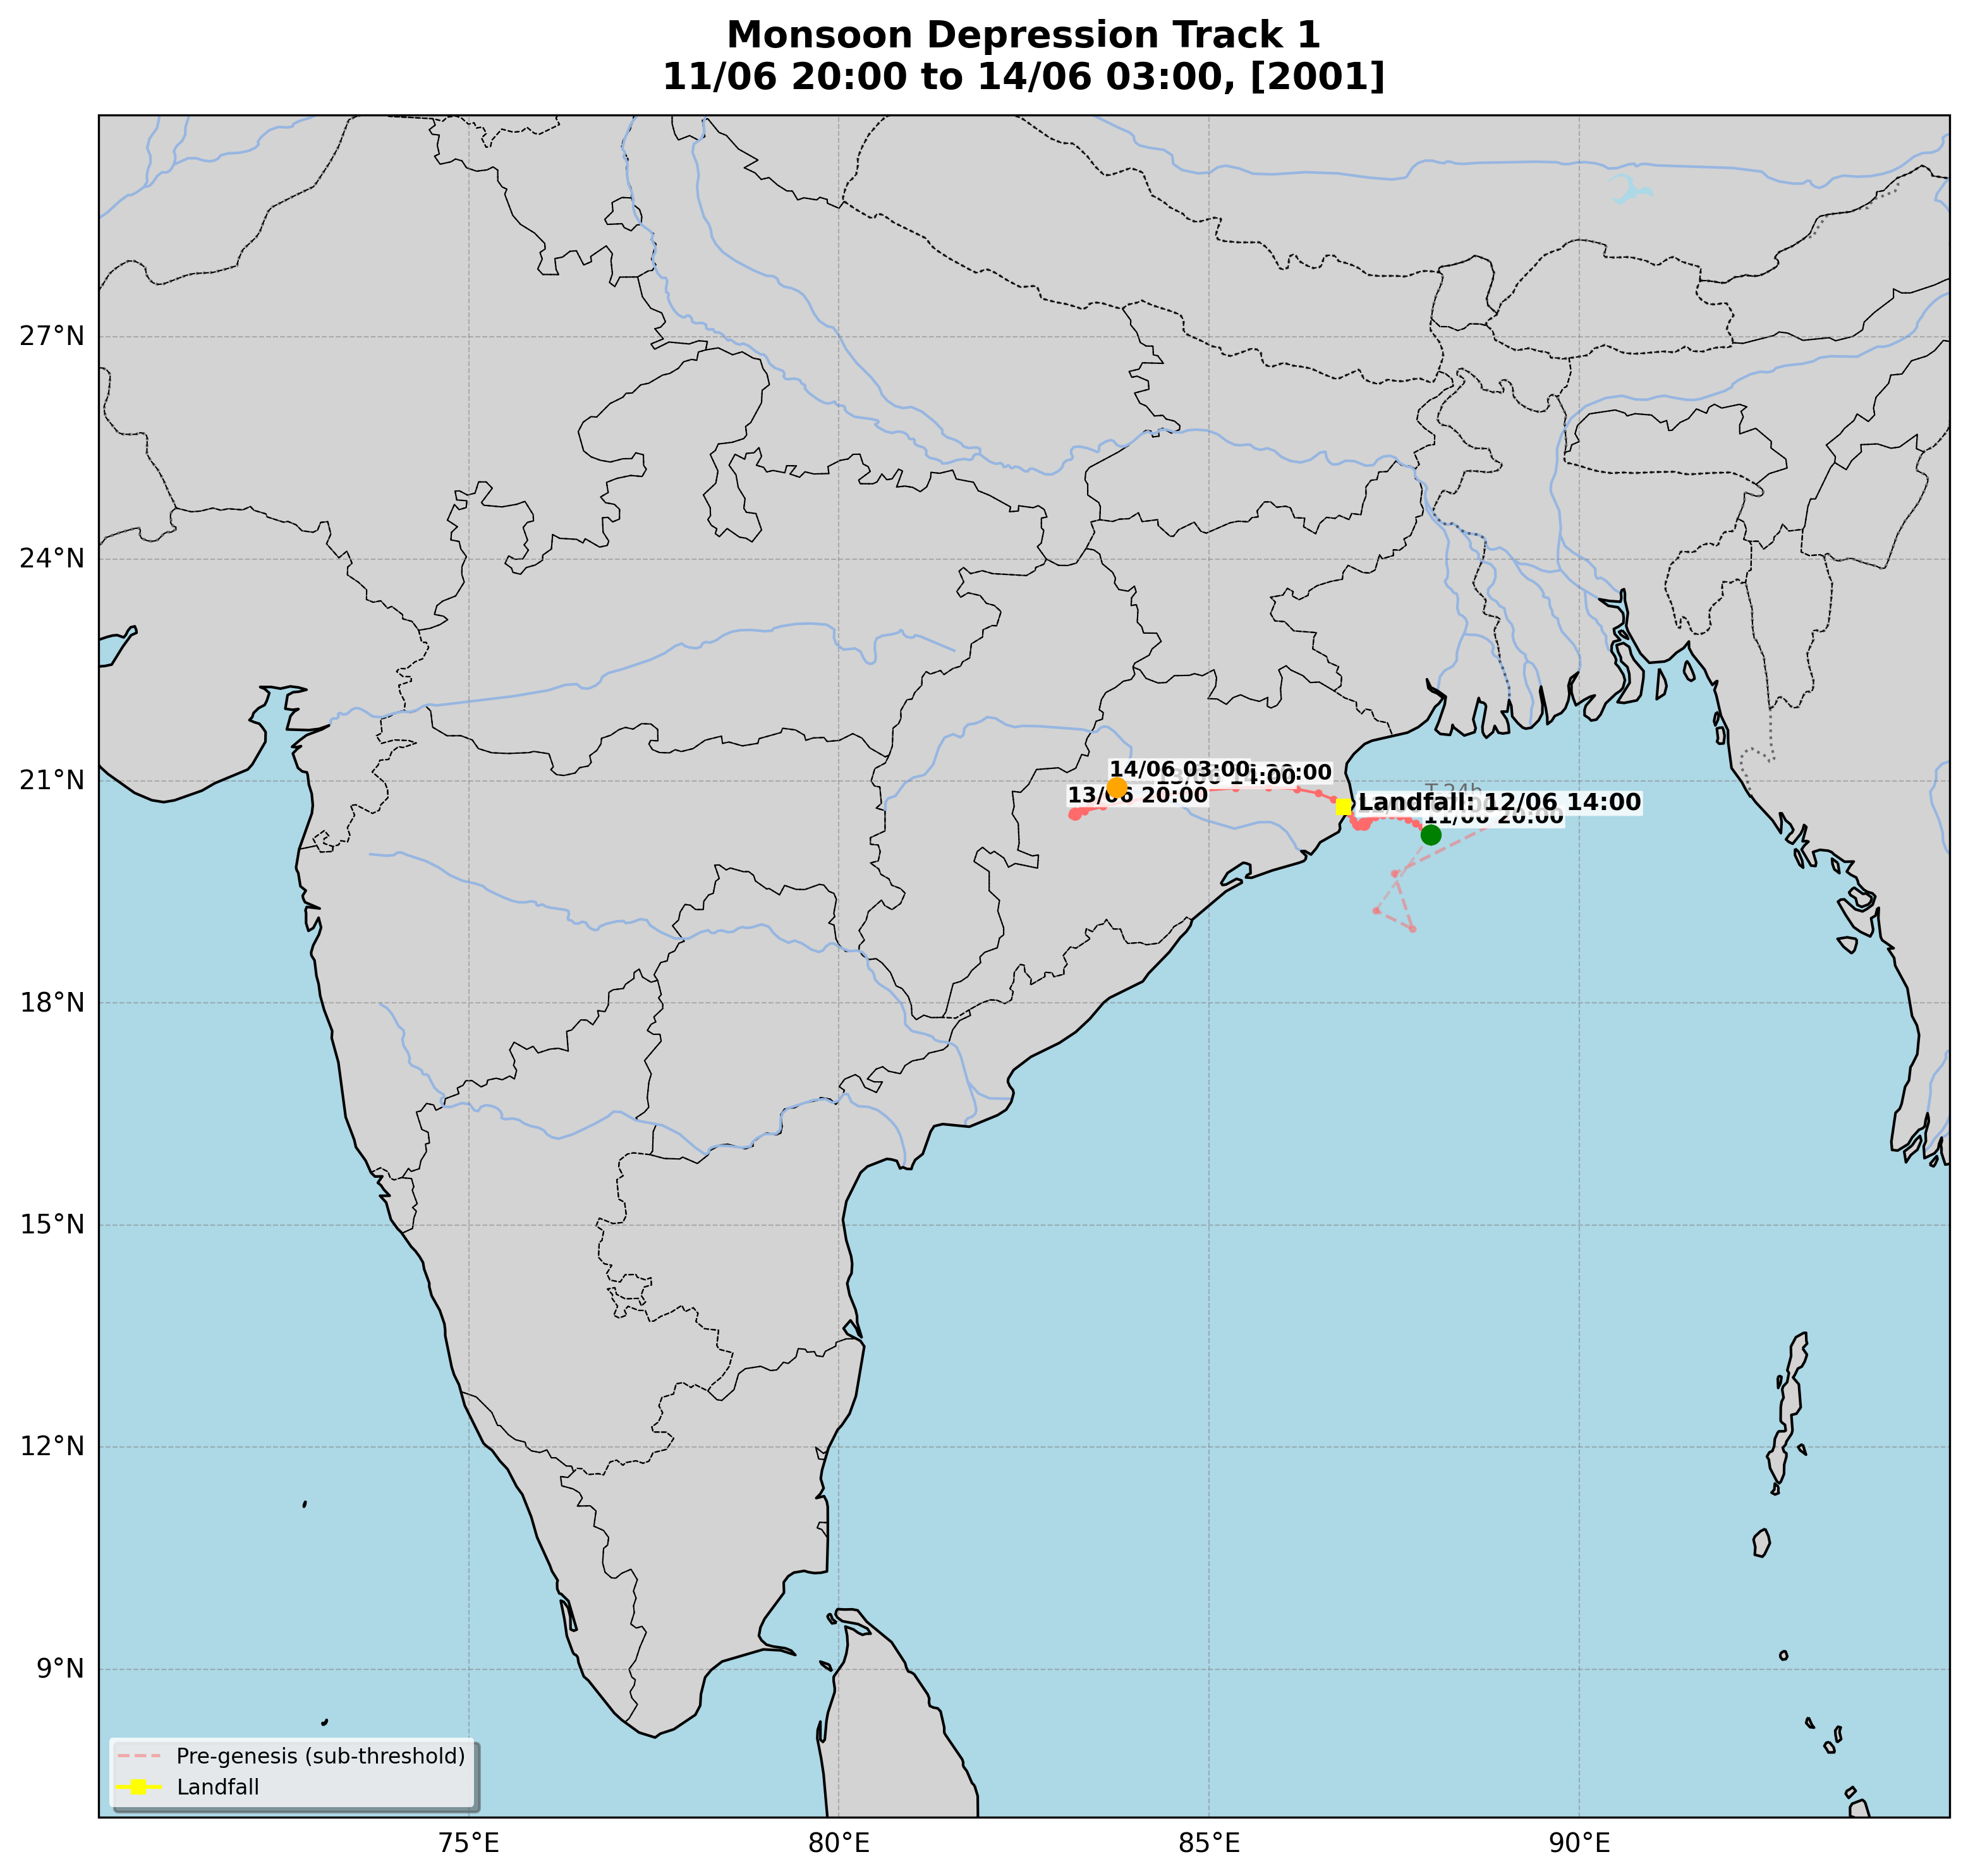
\includegraphics[width=0.67\textwidth]{track_short_spatial}
  \caption{Short-lived Track (June 2001), Non-BOE Track Path}
  \label{fig:tp_short_spatial}
\end{figure}

The above spatial track paths for the representative systems used in
the azimuthal analysis. The long-lived system exhibits a sustained
westward trajectory, whereas the short-lived system terminates on the
windward slopes of the terrain.

\subsection{Total Precipitation Dynamics}
\label{subsec:hovmoller_tp}

The evolution of total precipitation (\texttt{TP}) provides the most
visible evidence of the BOE mechanism. As shown in the representative
long-lived case, corresponding hovm\"oller plot
(Figure~\ref{fig:hovmoller_tp_long}), the MD
undergoes a structural regime shift.

In contrast, short-lived systems, corresponding hovm\"oller plot
(Figure~\ref{fig:hovmoller_tp_short}), exhibit a uniform radial
collapse. The absence of a sufficient land-surface energy source
leads to heavy precipitation at landfall leads to the simultaneous
dissipation of both core and peripheral convection within 24 hours of landfall.

\begin{figure}[H]
  \centering
  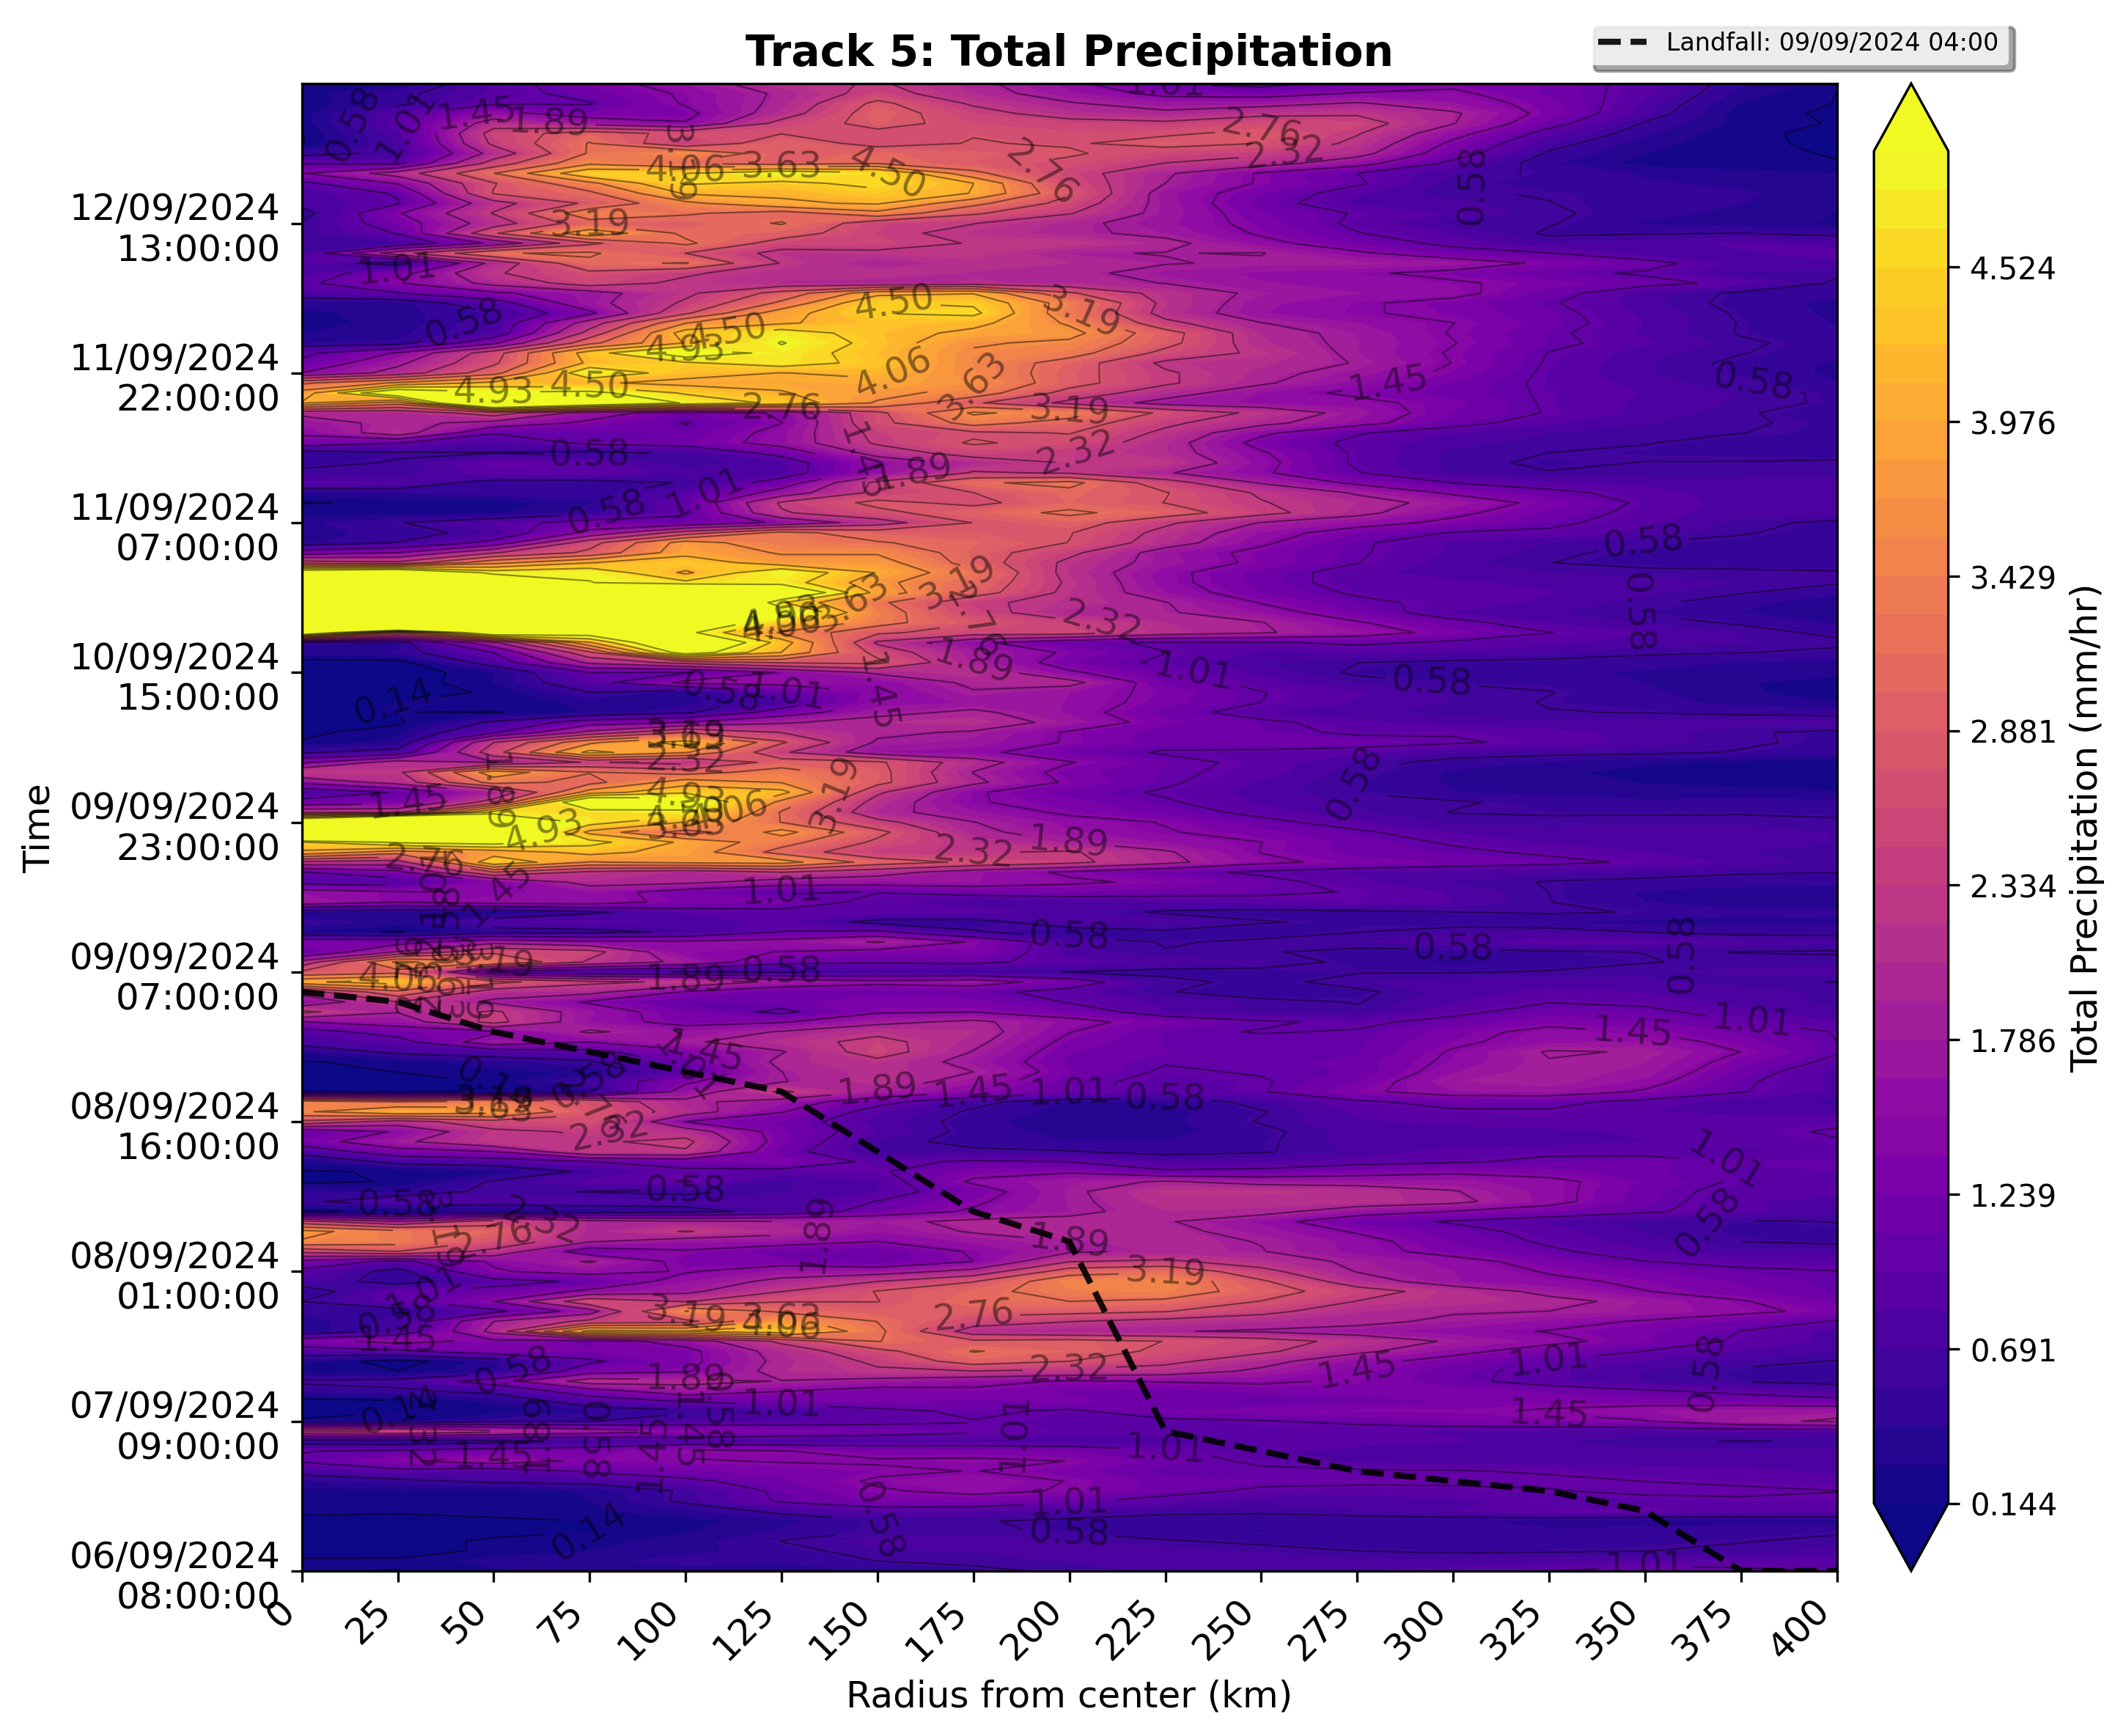
\includegraphics[width=0.69\textwidth]{track_long_tp_hov}
  \caption{Uniform precipitation after landfall}
  \label{fig:hovmoller_tp_long}
\end{figure}

\begin{figure}[H]
  \centering
  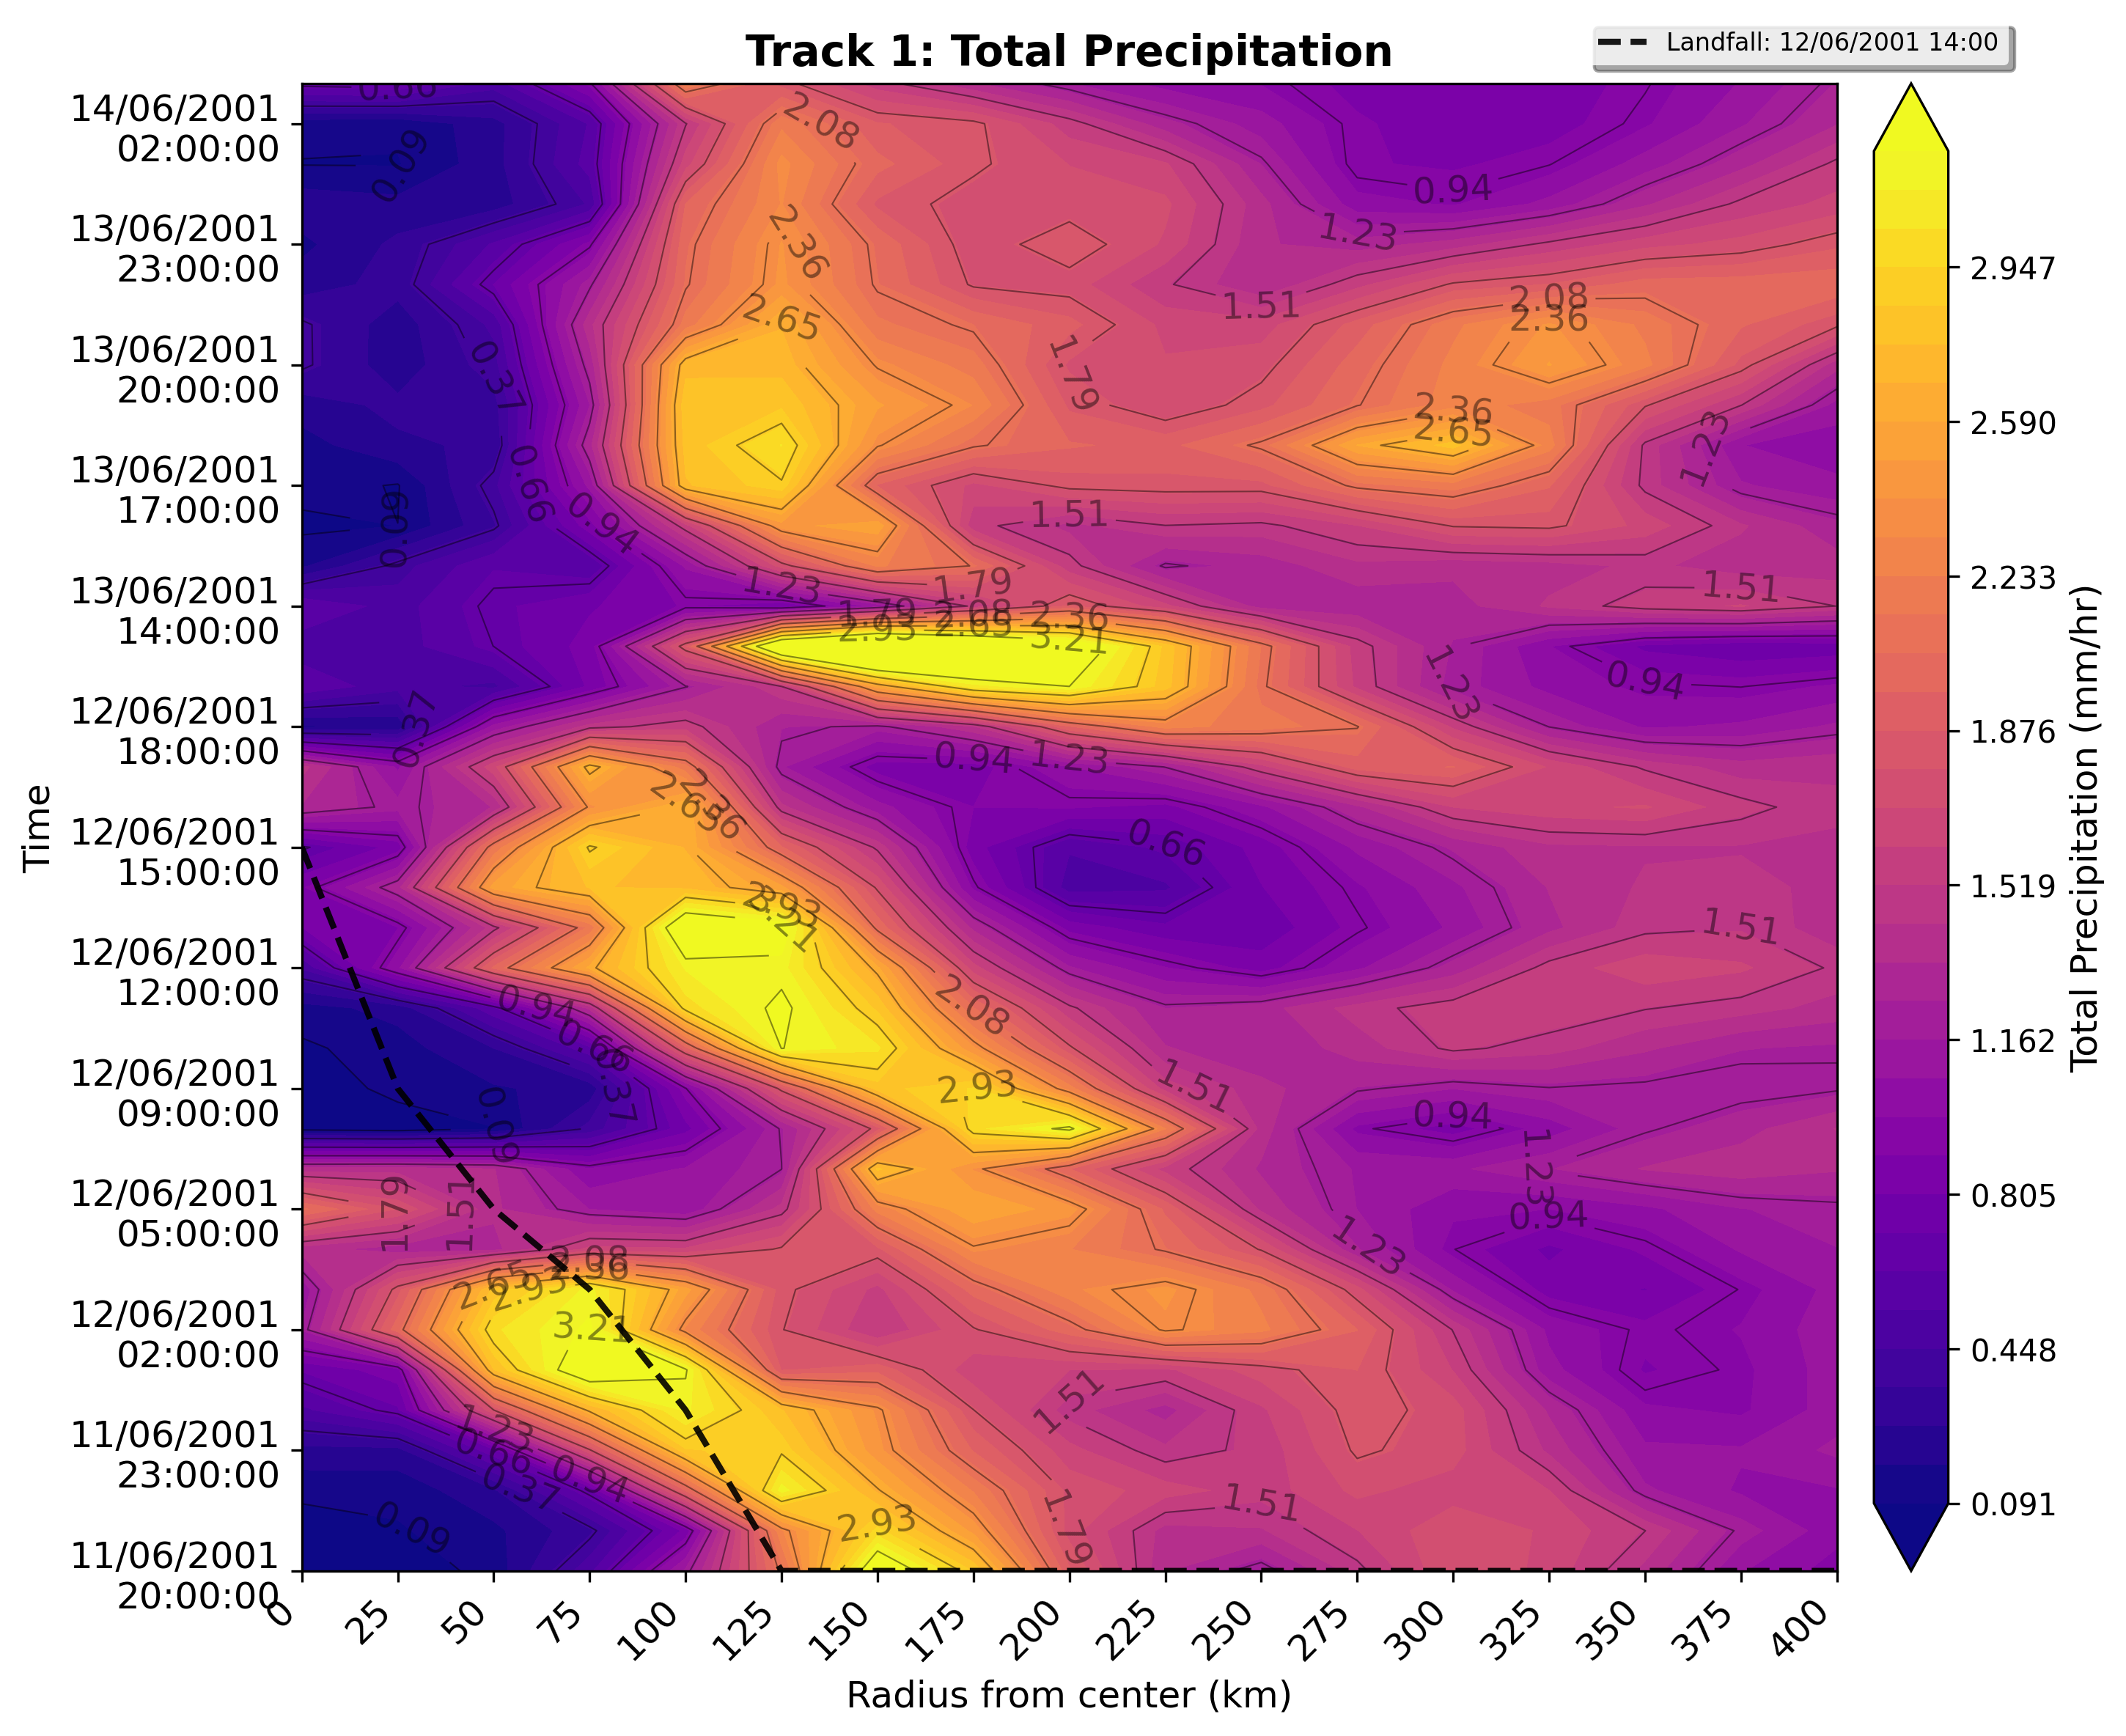
\includegraphics[width=0.69\textwidth]{track_short_tp_hov}
  \caption{Heavy precipitation at landfall}
  \label{fig:hovmoller_tp_short}
\end{figure}

% \caption{MD spatial track and Hovm\"{o}ller of precipitation. The
% long-lived system maintains its core rain-rate even after landfall.}
% \label{fig:hov_track_comparison_tp}

\subsection{Soil Moisture: Exposure Duration and Feedbacks}
\label{subsec:hovmoller_swvl1}

The Soil Water Volumetric level-1 (\texttt{SWVL1}) Hovm\"{o}ller
comparison (Figure~\ref{fig:hov_long_swvl1} and
\ref{fig:hov_short_swvl1}) reveals a critical temporal distinction in
surface energy availability. While both long-lived and short-lived
systems encounter similar absolute volumetric ranges (approximately
0.24-0.43\,m$^3$\,m$^{-3}$), their interaction with this moisture
reservoir differs in two key ways:

\textbf{Sustained Inland Exposure:} In the long-lived (BOE-active)
case (Figure~\ref{fig:hov_long_swvl1}), the system maintains
exposure to high soil moisture levels ($\gtrsim
0.38$\,m$^3$\,m$^{-3}$) for more than 72 hours post-landfall. This
extended exposure time with moist soil allows the system to continuously extract
latent heat as it traverses the Gangetic Plain.

\textbf{The Self-Wetting Signal:} Post-landfall ($t > 0$), the
long-lived MD displays a widening saturated core at radii
$<100$\,km. This is the evidence of a self-wetting feedback: the
storm's own precipitation replenishes the soil moisture,preventing
the rapid surface drying that typically follows landfall.

In contrast, while short-lived systems may encounter initially moist
soils (Figure~\ref{fig:hov_short_swvl1}) the duration of this
exposure is significantly truncated. Convective organization
collapses within 24 hours, often before the self-wetting feedback can
establish a stable energy-limited evaporation regime. This suggests
that the \textbf{persistence of the moist surface contact}, rather
than just the initial value, is the true gatekeeper of MD longevity.

\begin{figure}[H]
  \centering
  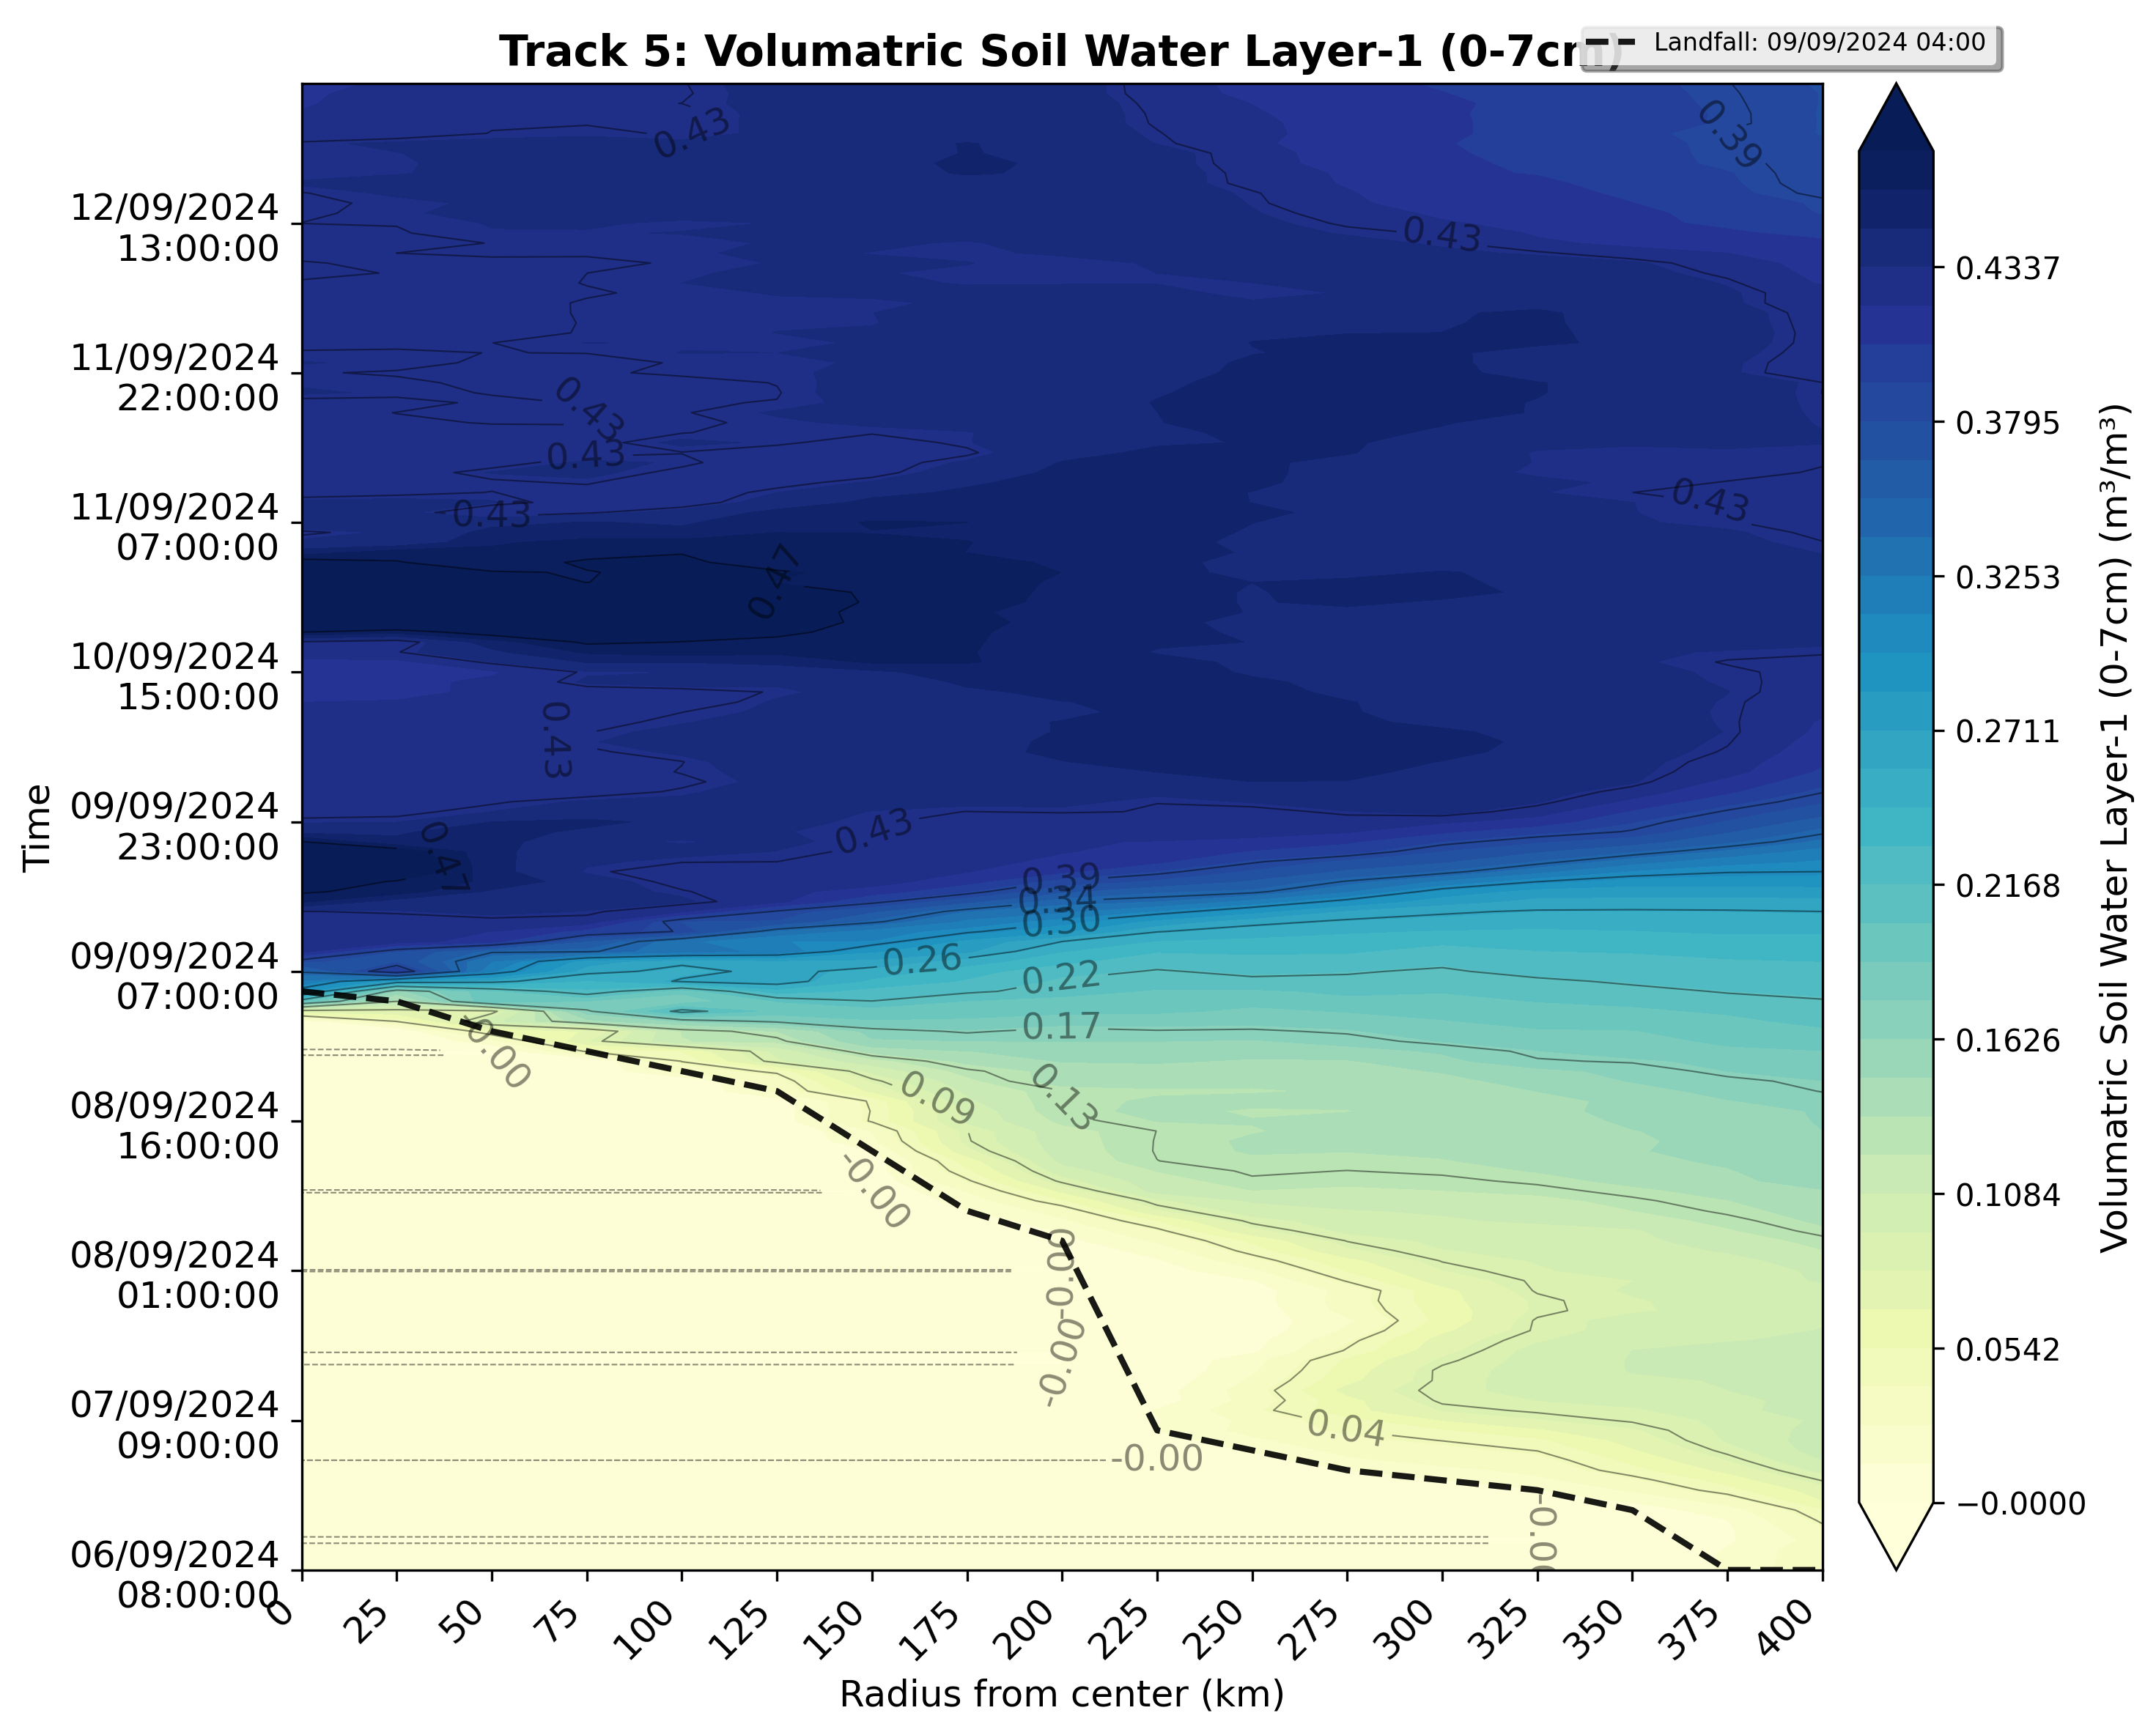
\includegraphics[width=0.69\textwidth]{track_long_swvl1_hov}
  \caption{BOE: Extended exposure to moist surface}
  \label{fig:hov_long_swvl1}
\end{figure}

\begin{figure}[H]
  \centering
  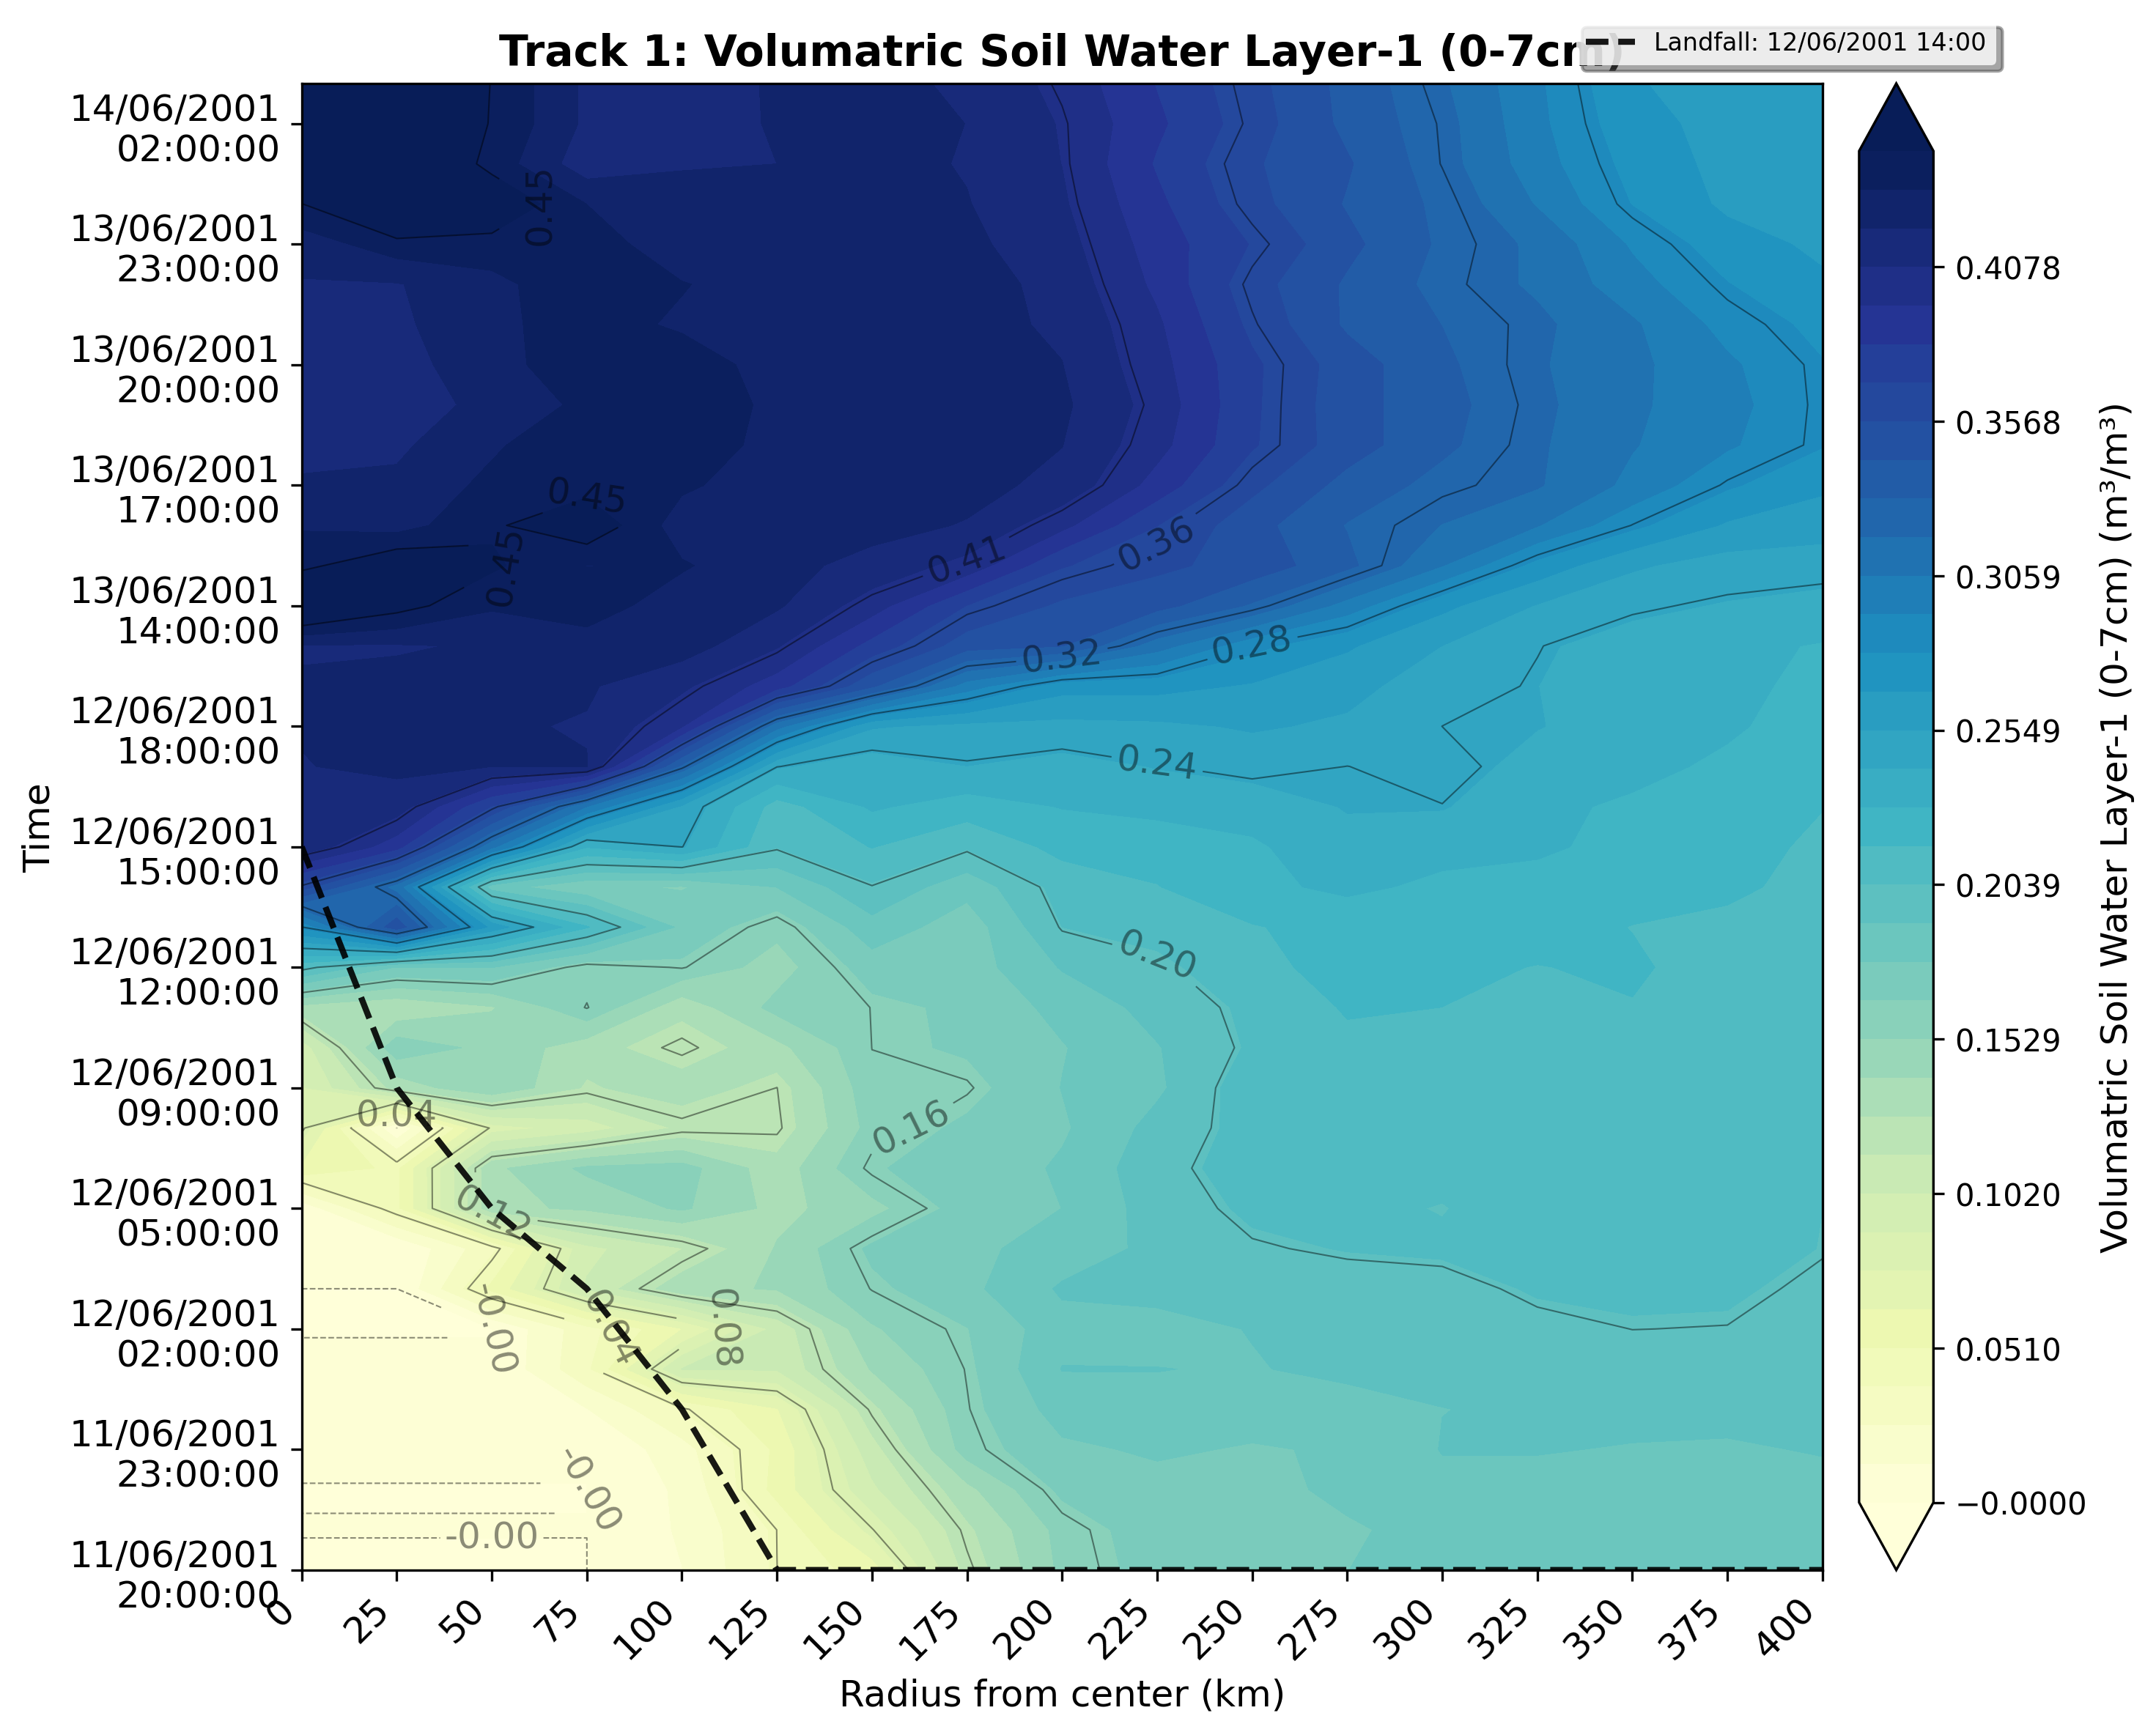
\includegraphics[width=0.69\textwidth]{track_short_swvl1_hov}
  \caption{Non-BOE: Rapid soil moisture decay}
  \label{fig:hov_short_swvl1}
\end{figure}

\subsection{Surface Latent Heat Flux: The BOE Energy Signal}
\label{subsec:hovmoller_slhtf}

The Surface Latent Heat Flux (\texttt{SLHTF}) provides the most direct measure
of the energy available to sustain the MD's secondary circulation. As
shown in Figure~\ref{fig:hov_long_slhtf} and \ref{fig:hov_short_slhtf}, both
long-lived and short-lived systems exhibit high oceanic LHF
magnitudes (ranging from $-220$ to $-150$\,W\,m$^{-2}$) prior to landfall.

The divergence in behavior occurs post-landfall ($t > 0$). In the
BOE-active case, the inner-core LHF stays effectively ``oceanic'' due
to the saturated soil state. This prevents the typical thermodynamic
decoupling that occurs when a storm moves over land. Conversely, in
non-BOE systems, the LHF is transient; the lack of a deep soil
moisture reservoir leads to a rapid collapse of the energy supply,
resulting in the dissipation of core convection.

\begin{figure}[H]
  \centering
  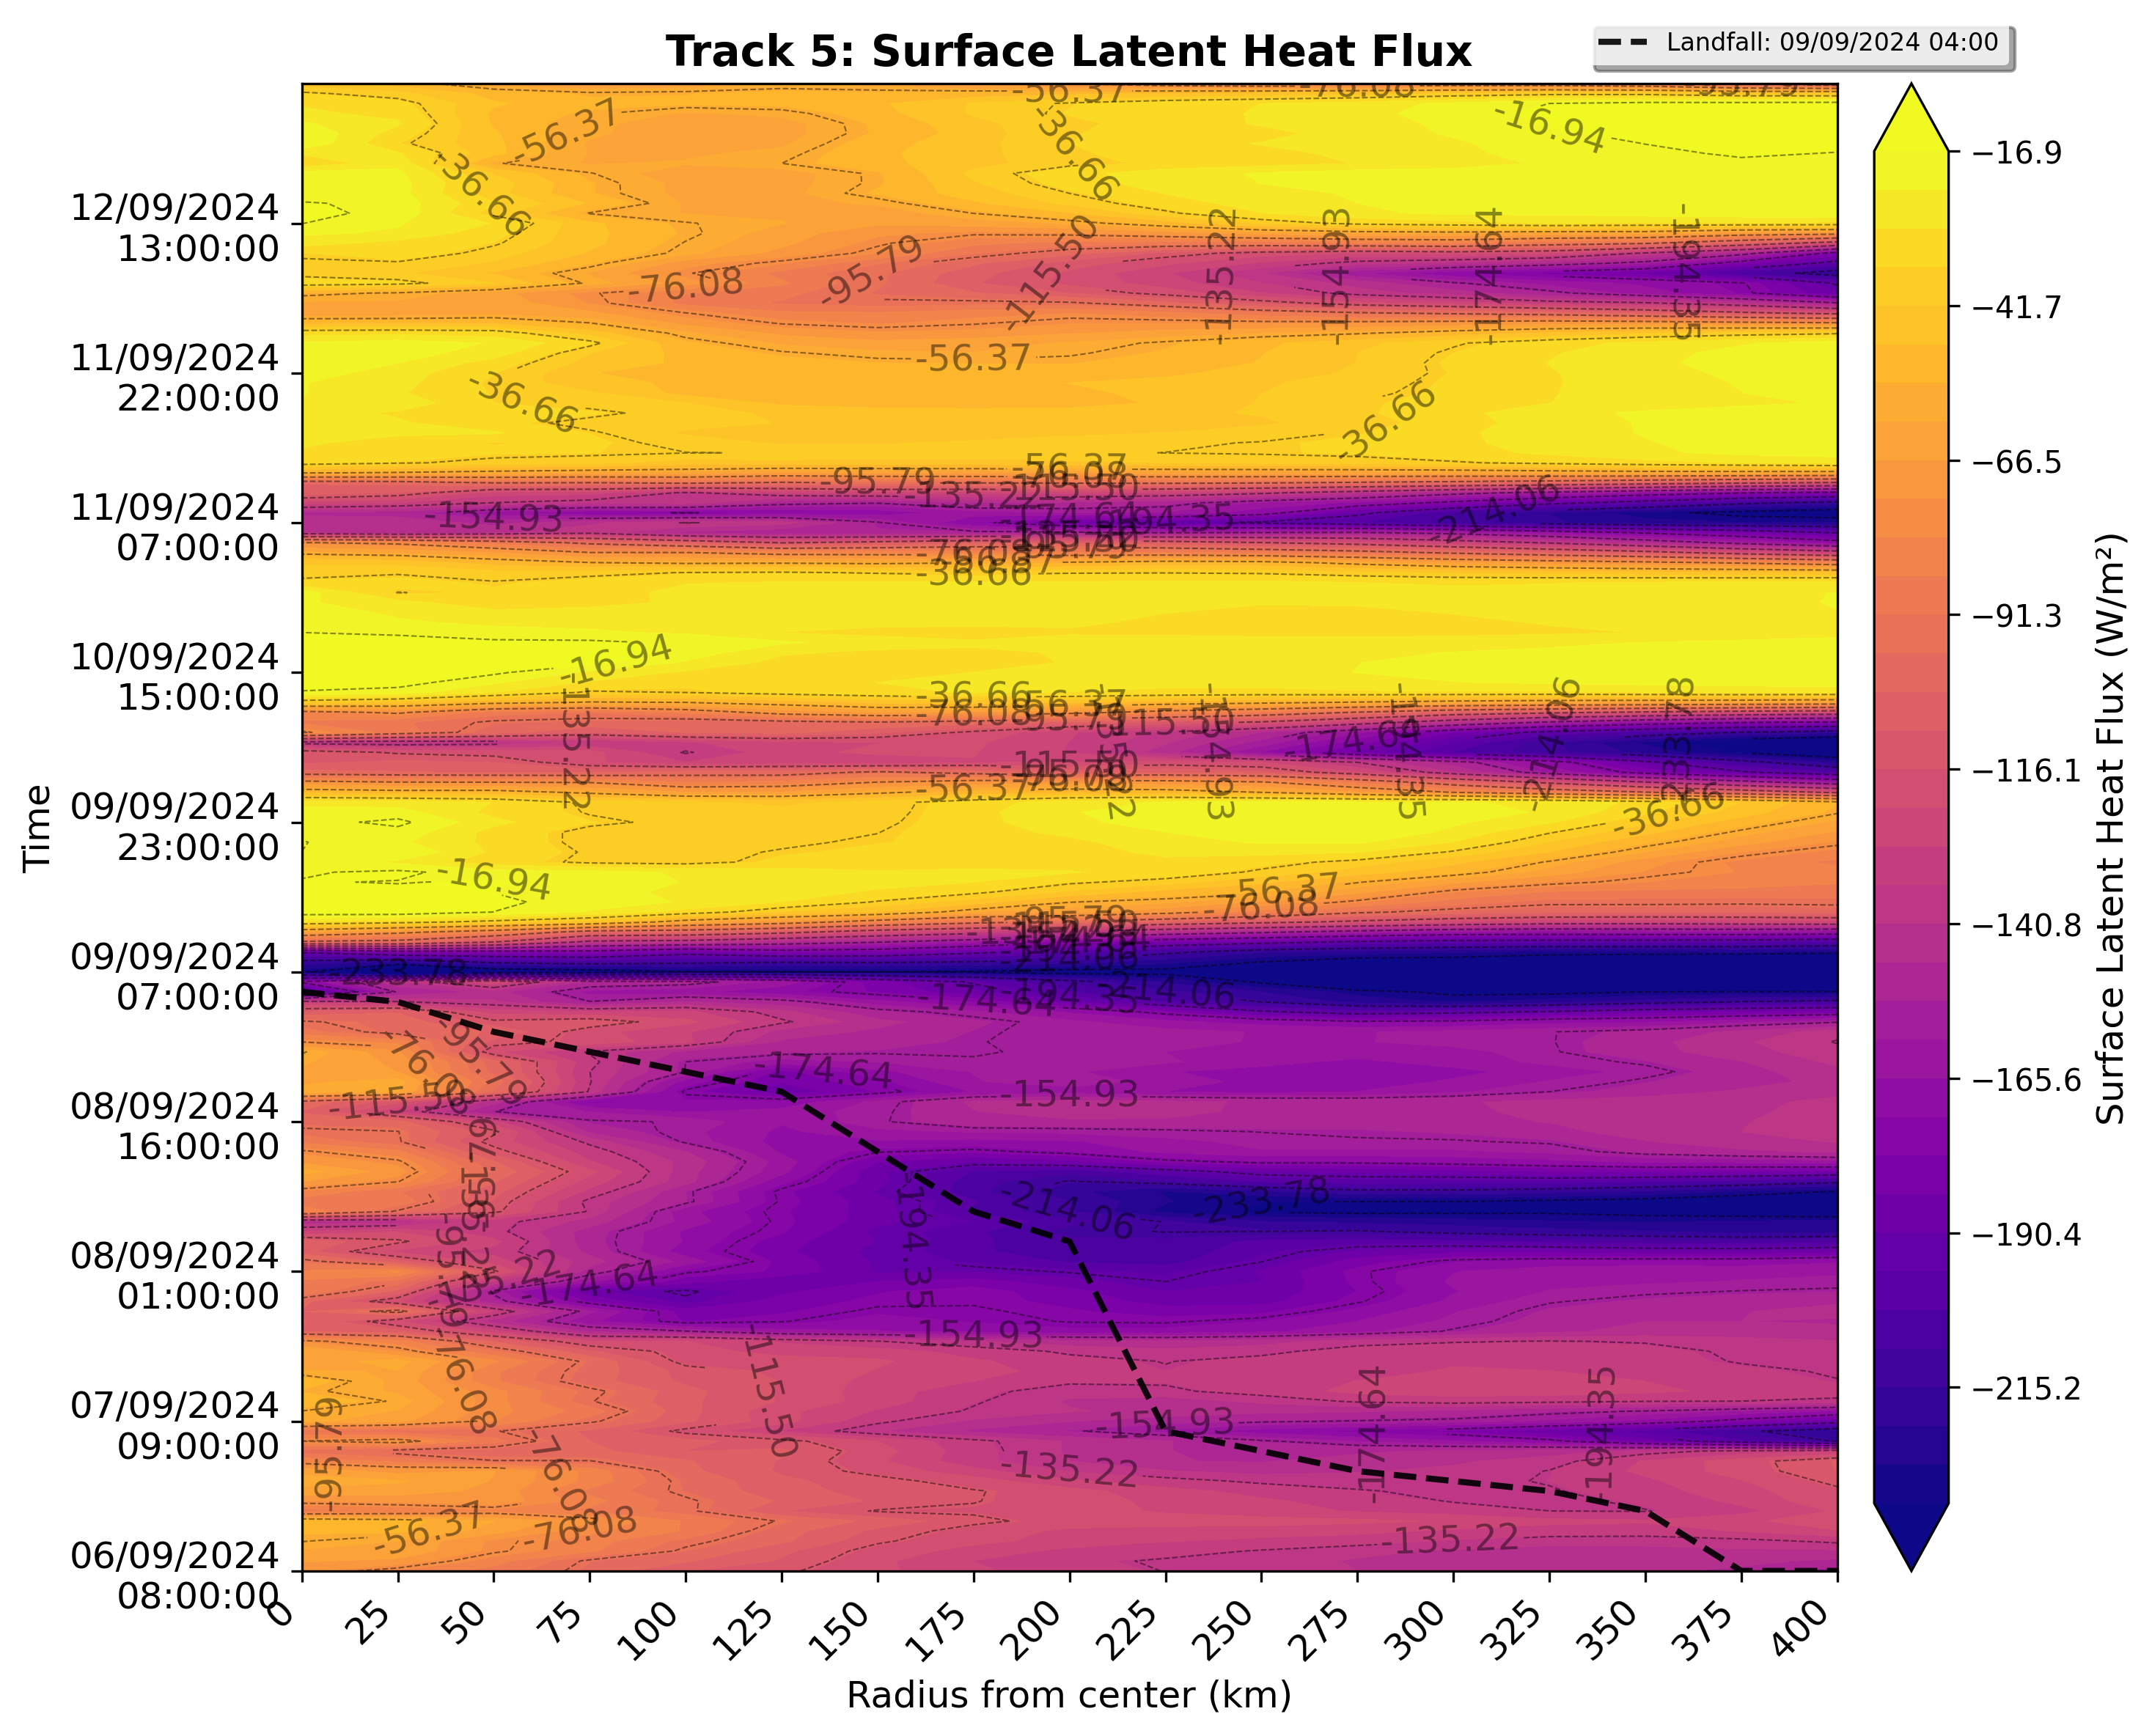
\includegraphics[width=0.69\textwidth]{track_long_slhtf_hov}
  \caption{BOE: Sustained land-phase flux}
  \label{fig:hov_long_slhtf}
\end{figure}

\begin{figure}[H]
  \centering
  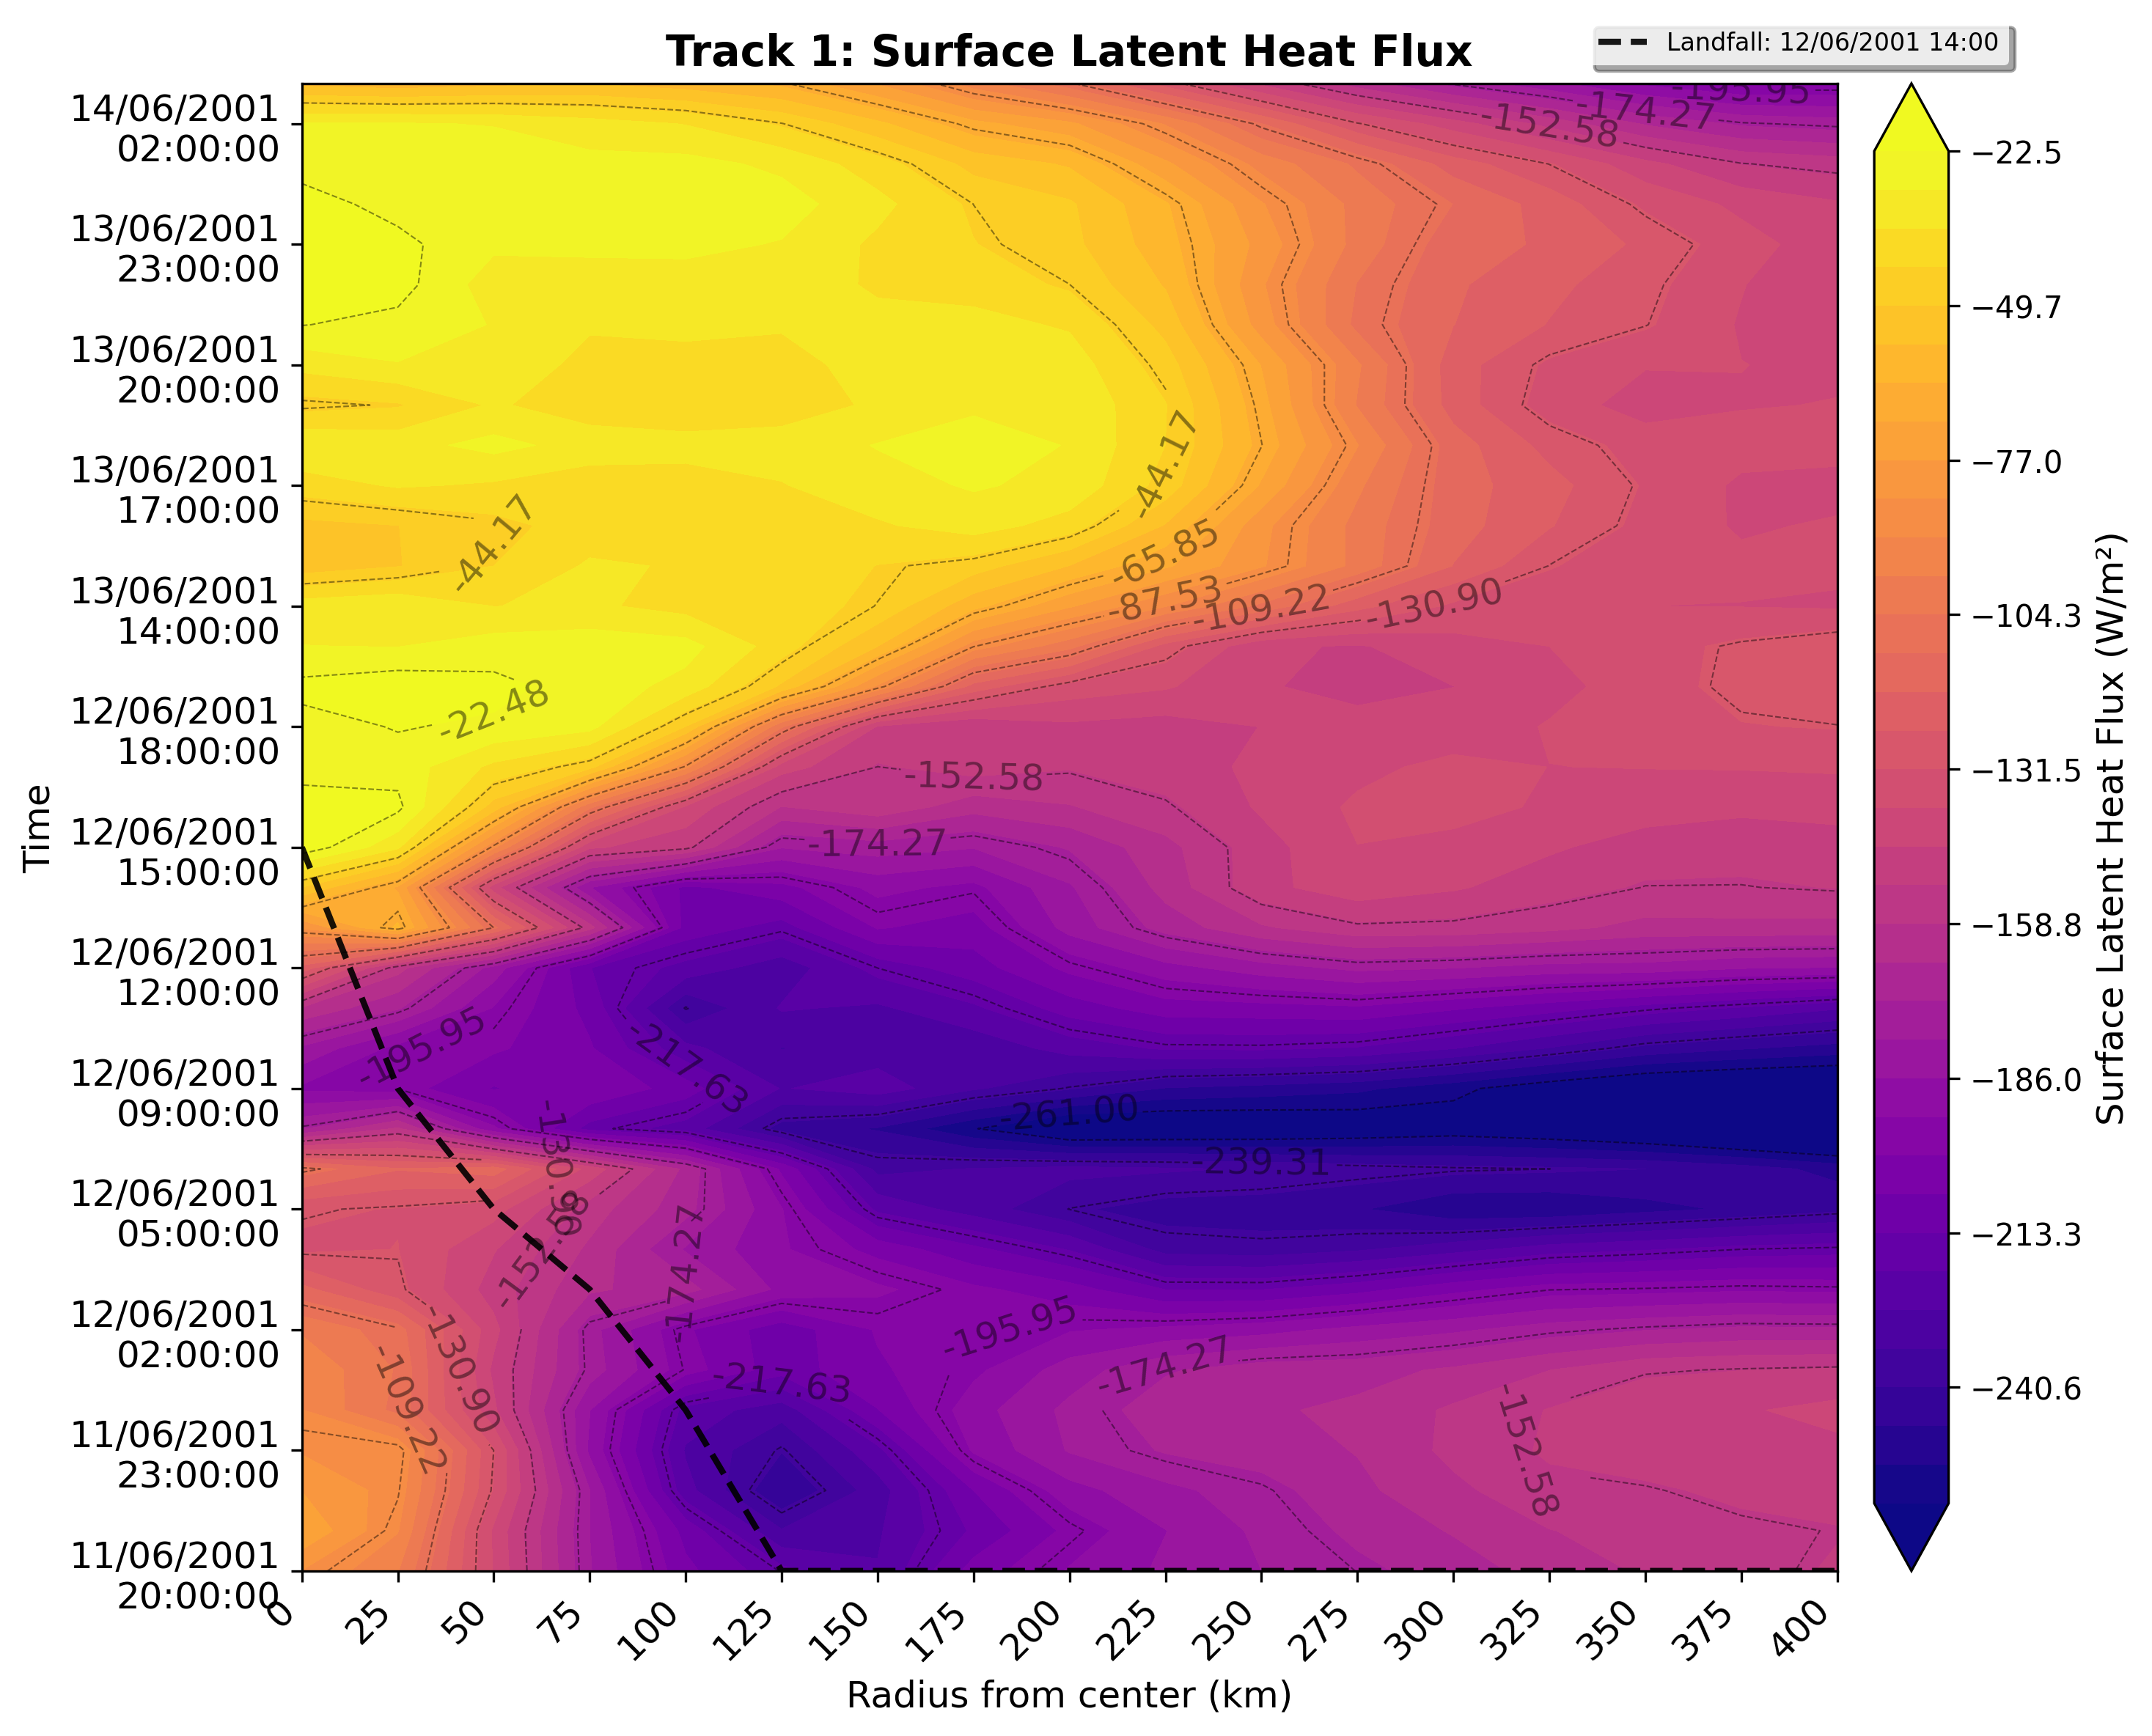
\includegraphics[width=0.69\textwidth]{track_short_slhtf_hov}
  \caption{Non-BOE: Transient flux collapse}
  \label{fig:hov_short_slhtf}
\end{figure}

Azimuthal Hovm\"{o}ller of Surface latent heat flux (\texttt{SLHTF})
(W\,m$^{-2}$), in the long-lived system
(Figure~\ref{fig:hov_long_slhtf}), LHF remains consistently above the
sustaining threshold ($>70$\,W\,m$^{-2}$) for over 48 hours inland.
While in the short-lived system (Figure~\ref{fig:hov_short_slhtf}),
the flux collapses within 12-18 hours of landfall despite similar
initial ranges.

\subsection{Surface Sensible Heat Flux: Thermal Feedback}
\label{subsec:hovmoller_ishf}

The Surface Sensible Heat Flux (\texttt{ISHF}) diagnostics
(Figure~\ref{fig:hov_long_ishf} and \ref{fig:hov_short_ishf}) reveal
the thermal state of the boundary layer. Over the ocean, both systems
maintain near-neutral SHF values ($-12$ to $-17$\,W\,m$^{-2}$),
indicating thermal equilibrium with the Bay of Bengal.

\begin{figure}[H]
  \centering
  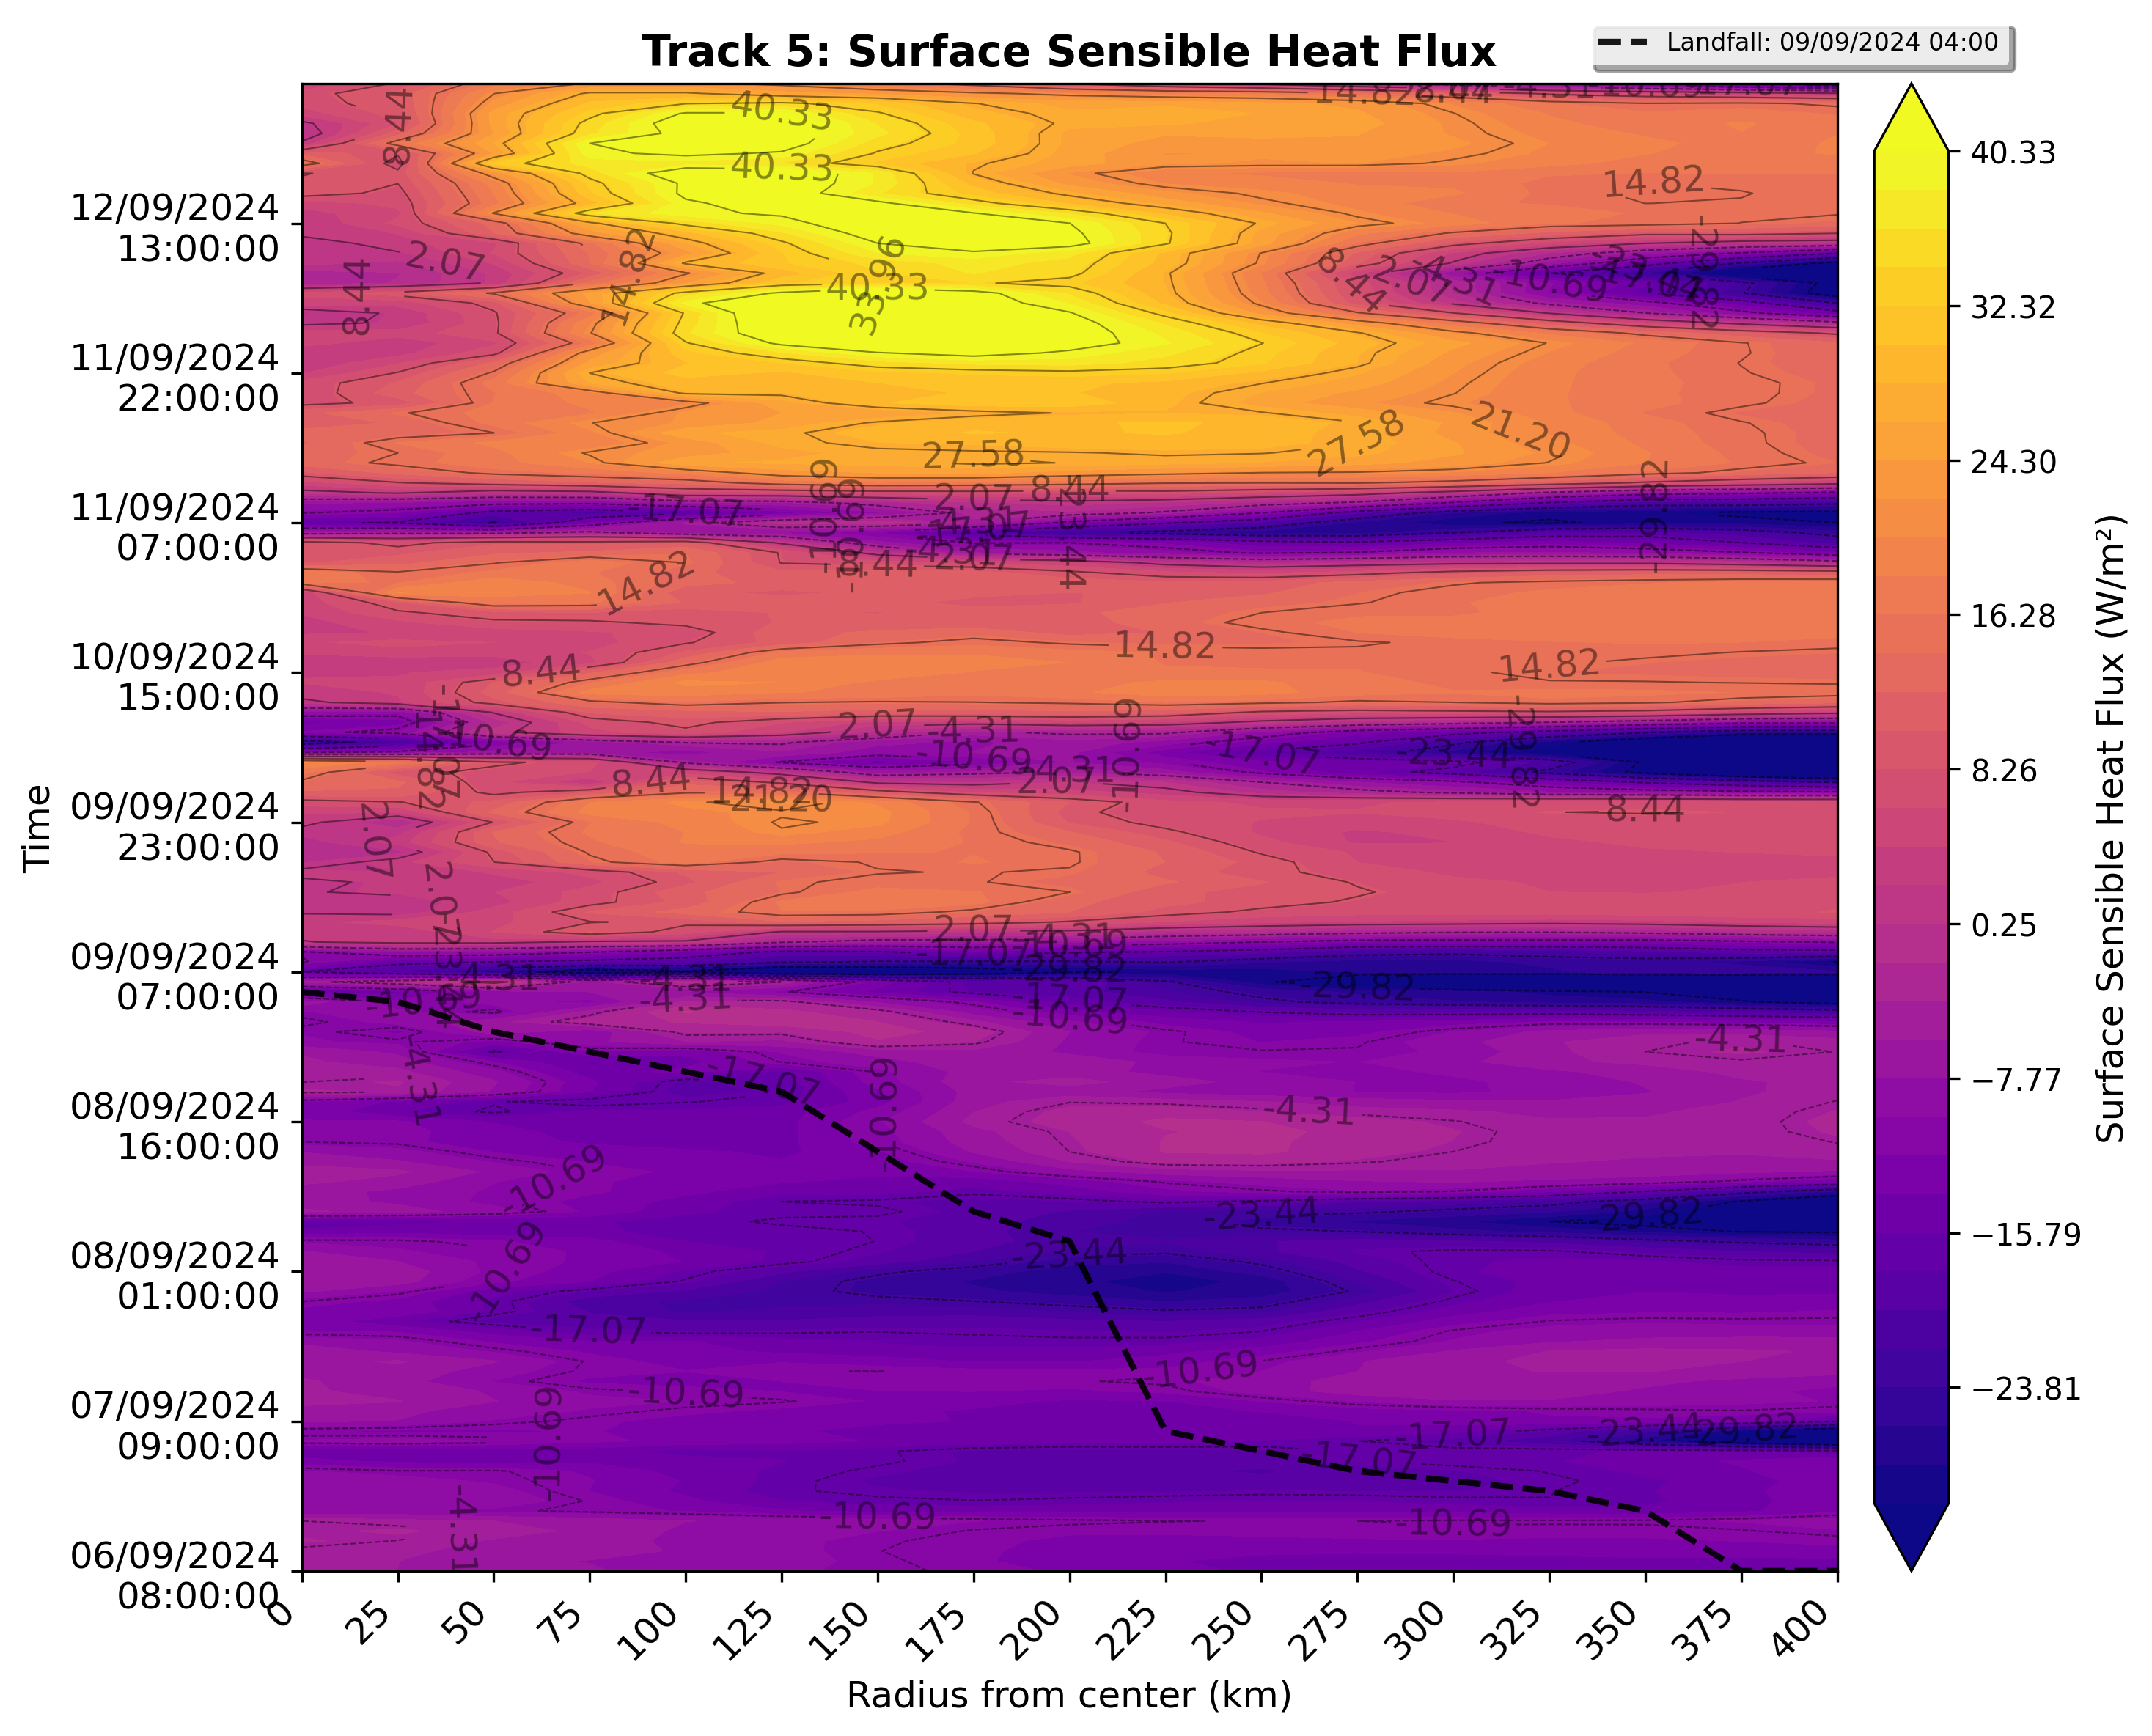
\includegraphics[width=0.67\textwidth]{track_long_ishf_hov}
  \caption{BOE: Suppressed sensible heating}
  \label{fig:hov_long_ishf}
\end{figure}

\begin{figure}[H]
  \centering
  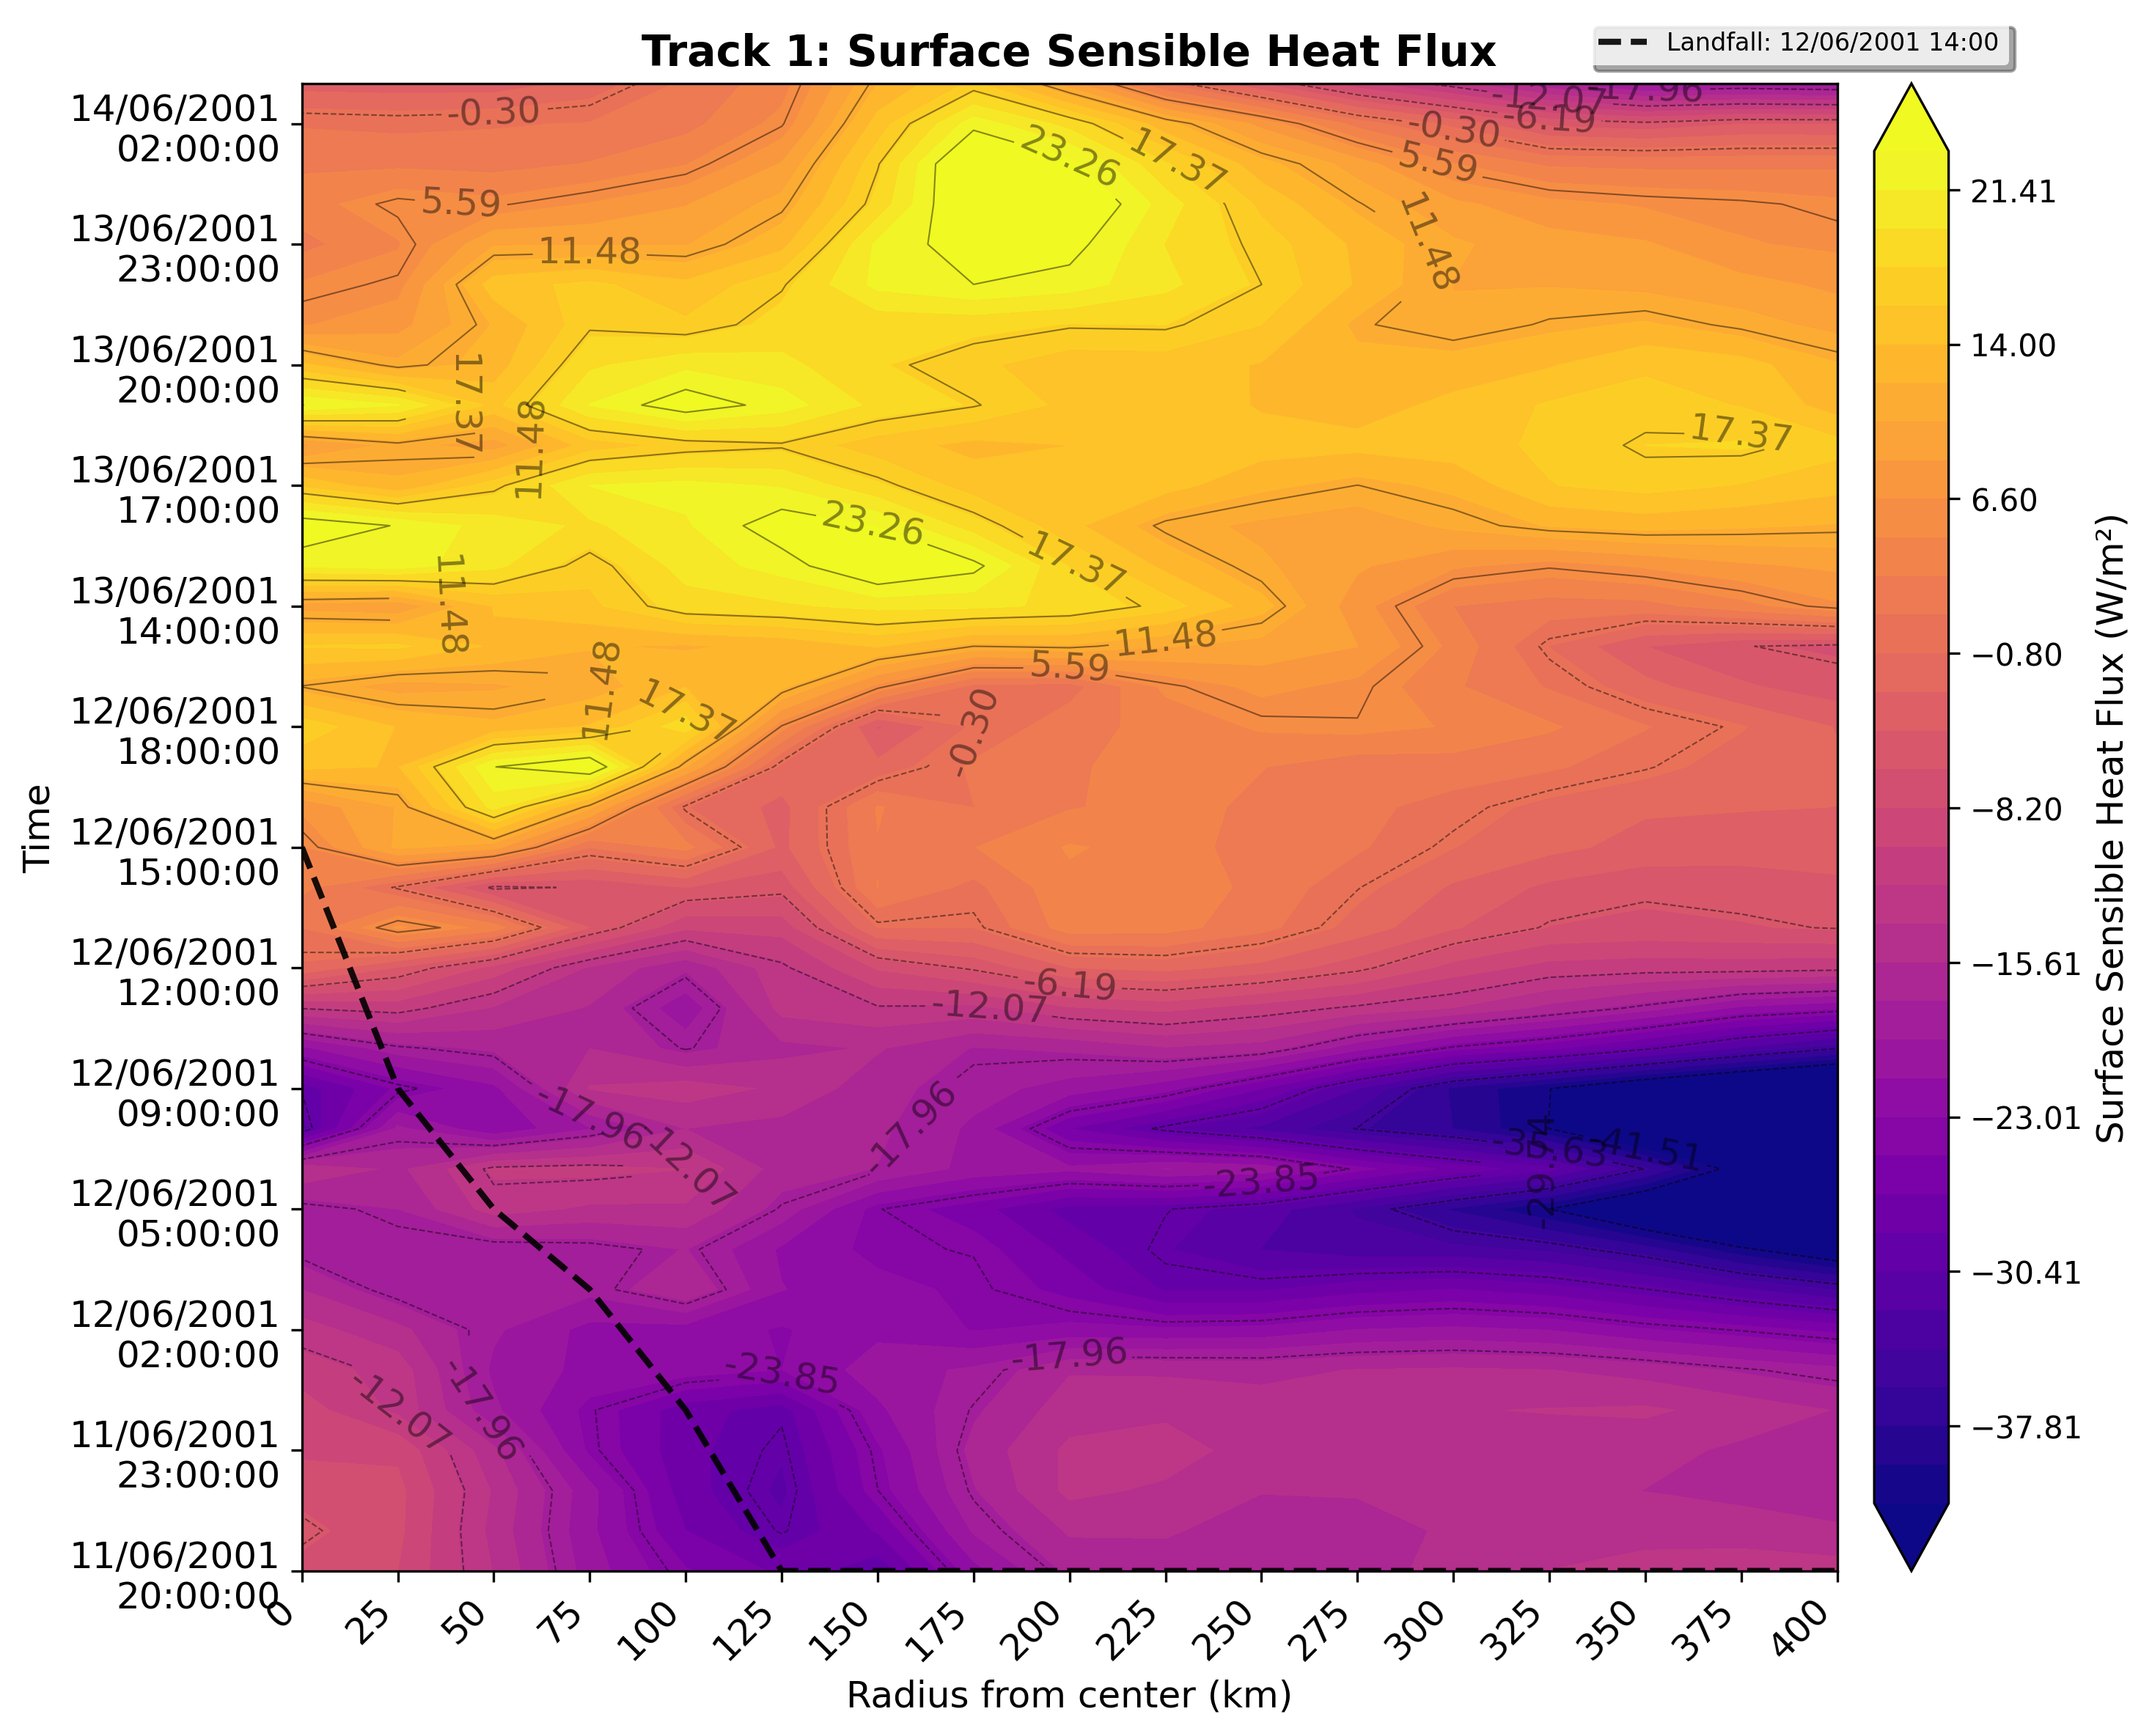
\includegraphics[width=0.67\textwidth]{track_short_ishf_hov}
  \caption{Non-BOE: Thermal destabilization}
  \label{fig:hov_short_ishf}
\end{figure}

Upon landfall, the BOE-active system (Figure~\ref{fig:hov_long_ishf})
maintains low Sensible heat flux on land; the energy is partitioned
into latent rather than sensible heat, keeping the inner core cool
and saturated, which is essential for vortex maintenance. In
contrast, the short-lived system encounters a stable thermal
environment, with SHF reaching extremes of 21\,W\,m$^{-2}$ (downward)
to $-37$\,W\,m$^{-2}$ (upward). This rapid sensible heating from a
dry surface increases the boundary layer height and encourages
dry-air entrainment.

Azimuthal Hovm\"{o}ller of SSHF (W\,m$^{-2}$). The non-BOE system
(Figure~\ref{fig:hov_short_ishf}) shows extreme fluctuations at
landfall (ranging from 21 to $-37$\,W\,m$^{-2}$), indicating a hot,
dry surface that disrupts the saturated inner-core structure after
encountering landfall.

\subsection{Dew Point Temperature: Boundary Layer Saturation and Maintenance}
\label{subsec:hovmoller_d2m}

% The 2-m dew point temperature ($d2m$) Hovm\"{o}ller results
% (Figure~\ref{fig:hov_track_comparison_d2m}) serve as a diagnostic for
% the moisture state of the boundary layer, complementing the energy
% flux analysis in Section~\ref{subsec:hovmoller_slhtf}. While both
% long-lived and short-lived systems eventually reach a minimum dew
% point of $\sim$295\,K, the \textbf{timescale of desipation} varies
% significantly, marking the difference between a system that carries
% its environment inland and one that succumb to continental drying.

The azimuthal hovm\"{o}ller evolution of 2-m dew point temperature
(\texttt{D2M}) illustrates how BOE-active systems maintain a
maritime-like boundary layer deep into the inland. While both
eventually settle toward a floor value of $\sim$295--296\,K, the
distinction lies in the \textbf{moisture decay rate} following landfall
(Figure~\ref{fig:hov_long_d2m} and \ref{fig:hov_short_d2m}).

\begin{figure}[H]
  \centering
  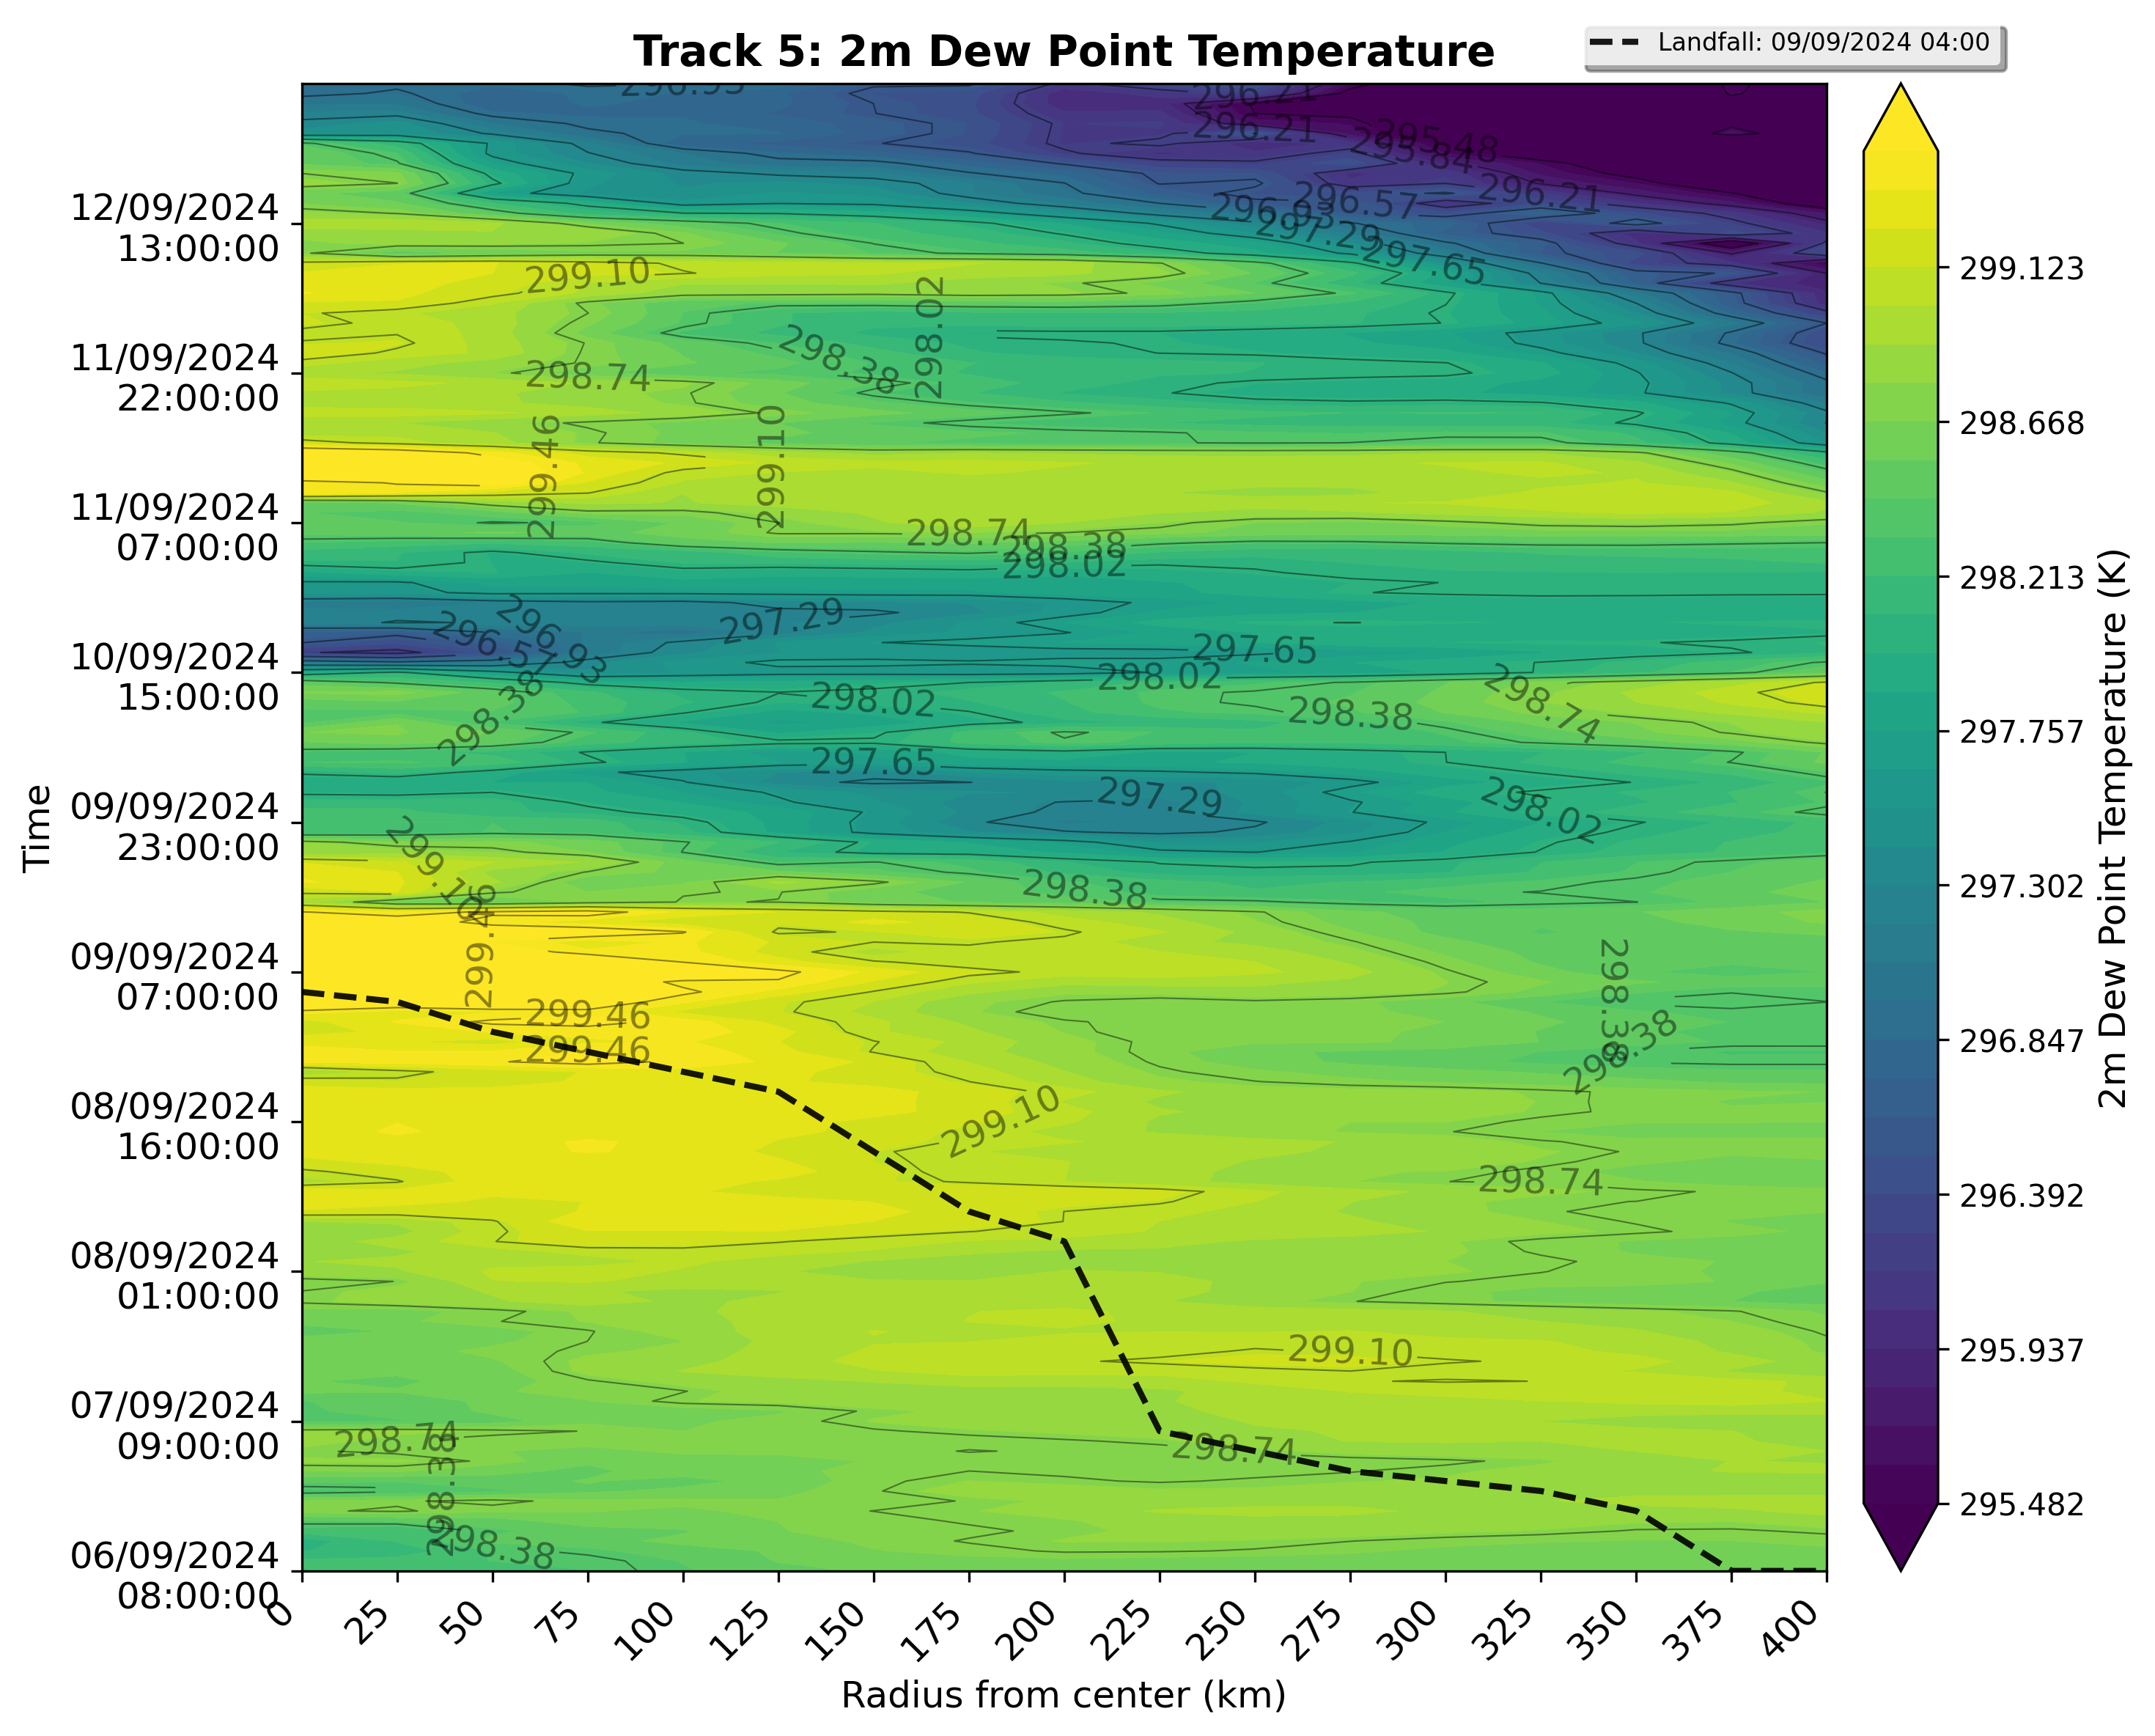
\includegraphics[width=0.69\textwidth]{track_long_d2m_hov}
  \caption{BOE: Sustained moisture saturation}
  \label{fig:hov_long_d2m}
\end{figure}

\begin{figure}[H]
  \centering
  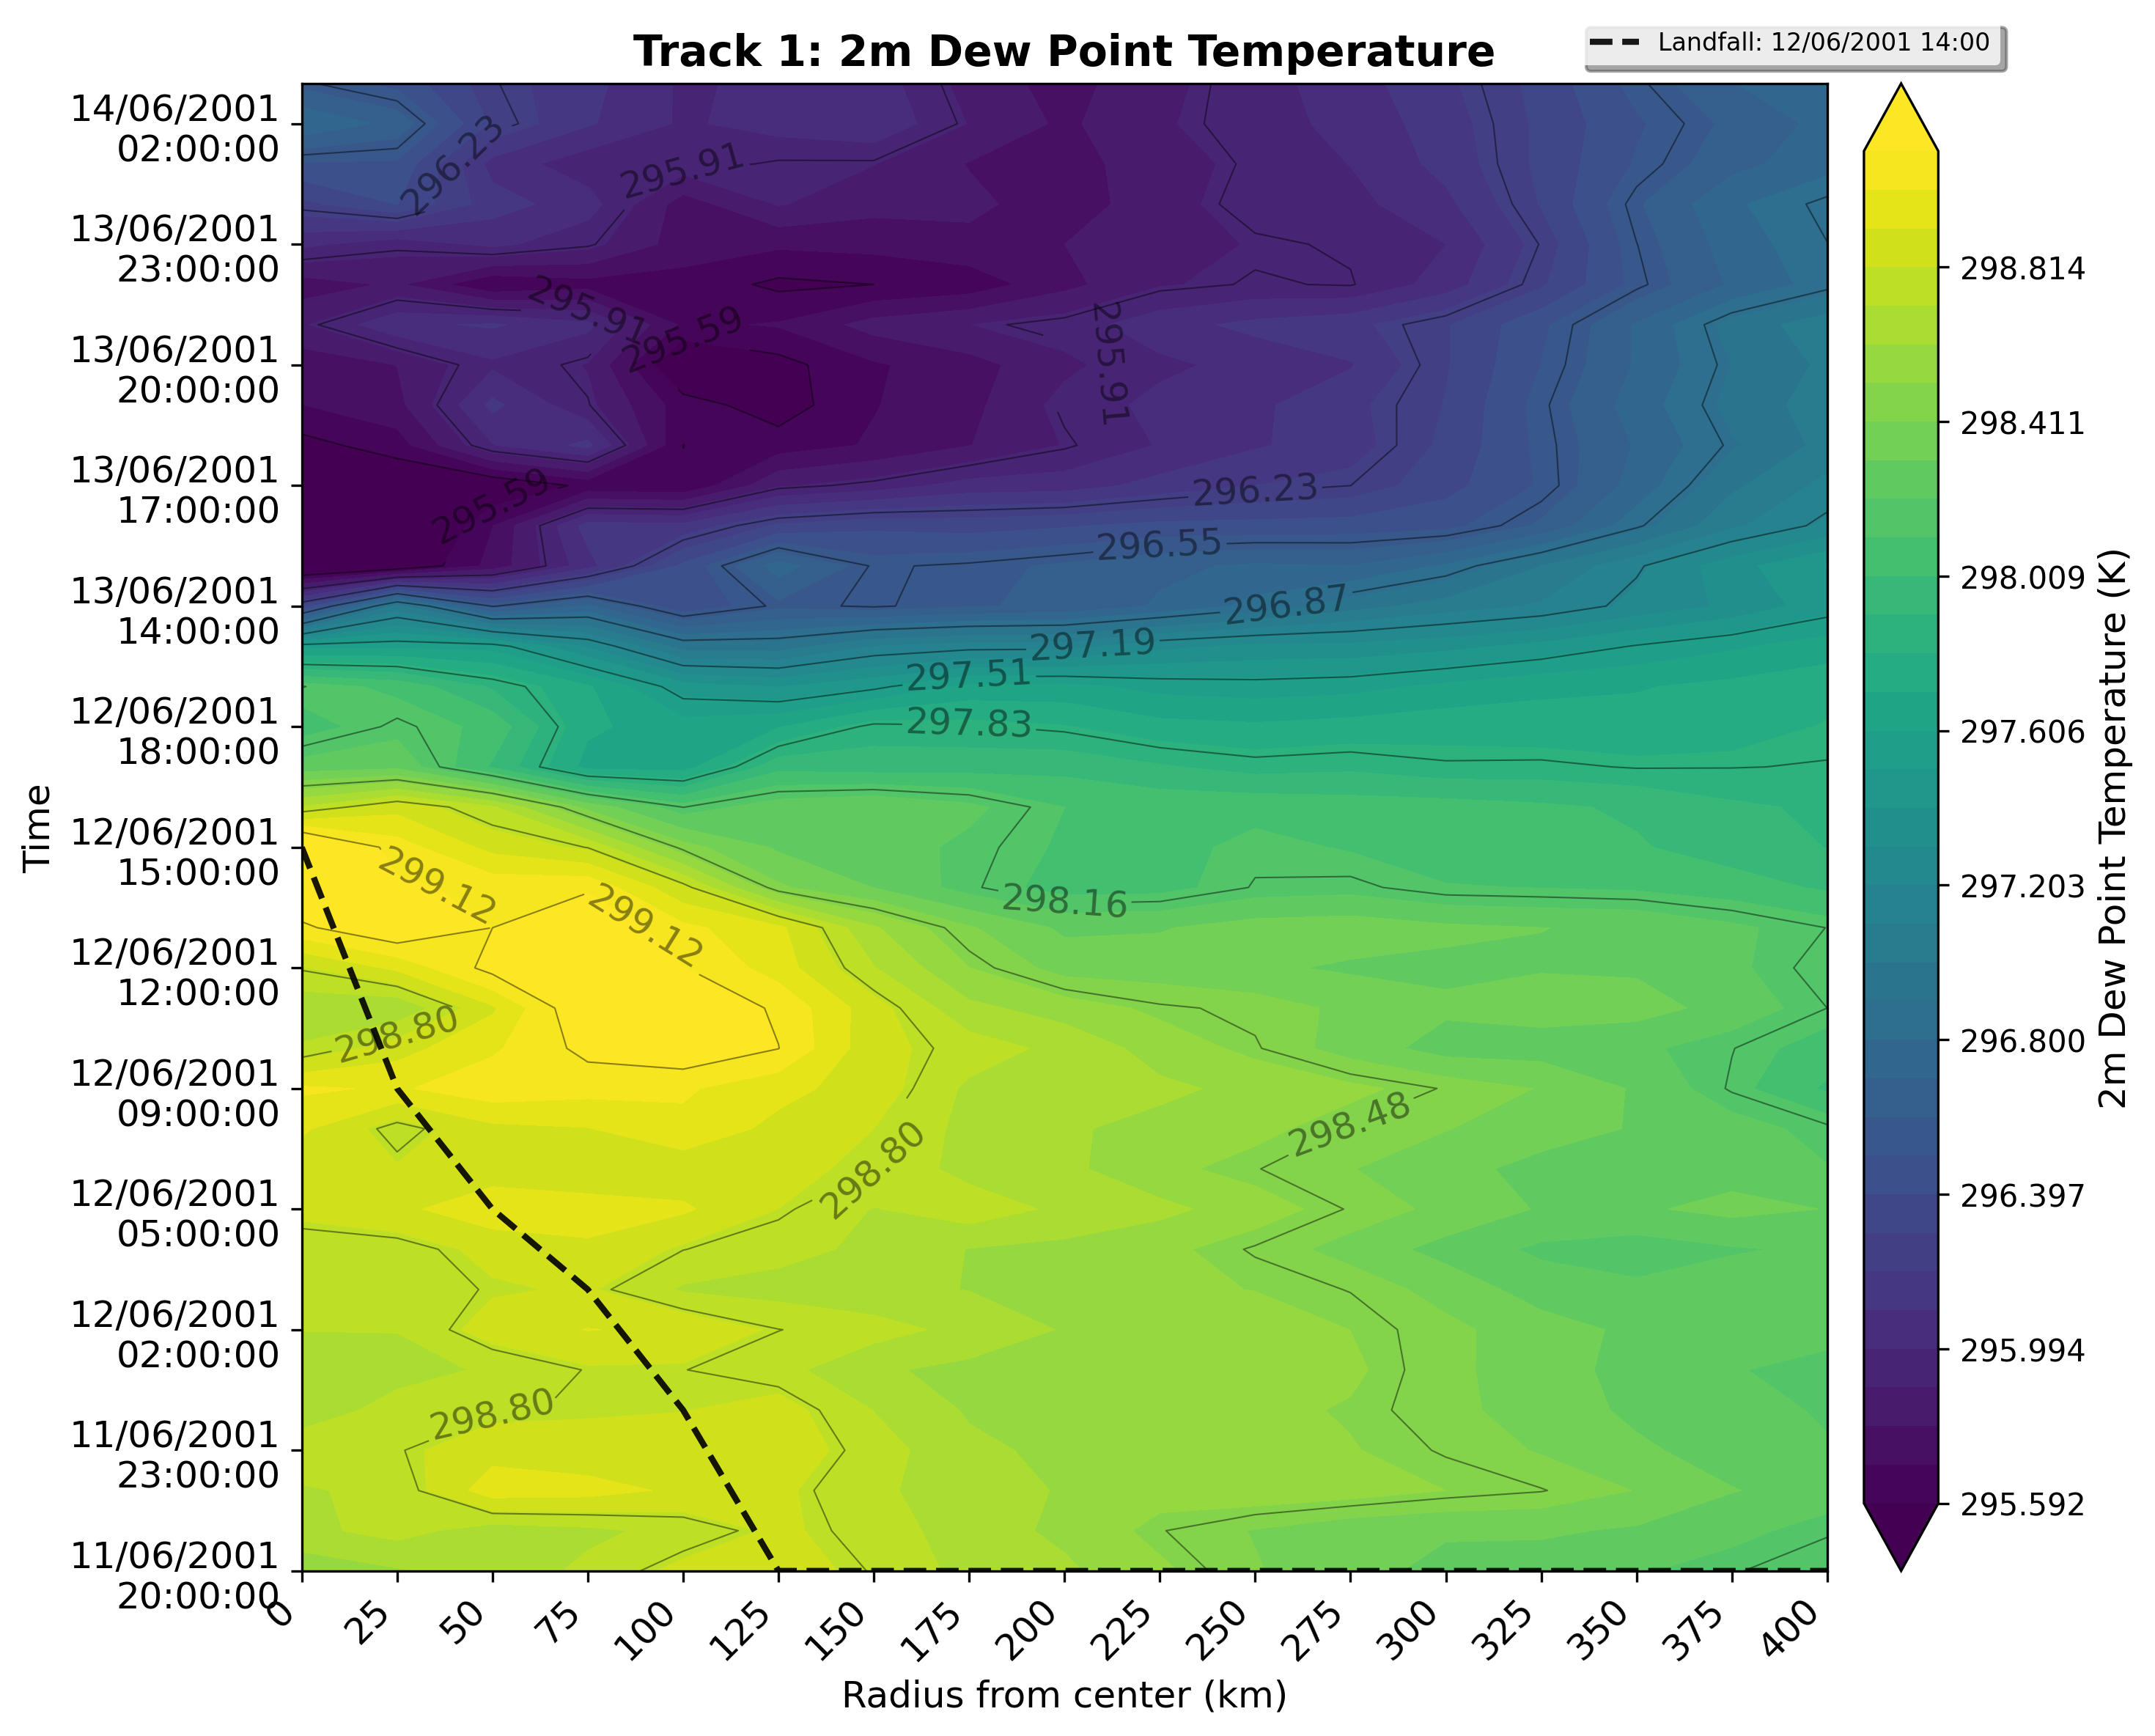
\includegraphics[width=0.69\textwidth]{track_short_d2m_hov}
  \caption{Non-BOE: Rapid boundary layer drying}
  \label{fig:hov_short_d2m}
\end{figure}

Azimuthal Hovm\"{o}ller of 2-m dew point temperature (\texttt{D2M}).
The long-lived system (Figure~\ref{fig:hov_long_d2m}) maintains a
high moisture floor ($>298$\,K) for over 72 hours, whereas the
short-lived system (Figure~\ref{fig:hov_short_d2m}) drops to values
almost immediately after landfall.

In a standard landfall scenario, the removal of the maritime moisture
source should trigger a rapid drop in \texttt{D2M}. This is observed in the
short-lived population (Figure~\ref{fig:hov_short_d2m}), where
\texttt{D2M} falls toward 296\,K within 12-24 hours. This drop increases
the Dew Point Depression (DPD), raising the Lifting Condensation
Level (LCL) and effectively dissipating the core convection.

However, long-lived MDs exhibit a moisture maintenance signal. By
sustaining \texttt{D2M} at 298--299\,K deep into the land phase and for
longer time period, these systems effectively carry their own
environment inland. This maintenance is a direct physical consequence
of the soil moisture and LHF feedbacks described in previous sections:
\begin{itemize}
  \item \textbf{Recycling:} The wet soil reservoir identified in
    Section~\ref{subsec:hovmoller_swvl1} evaporates moisture back
    into the boundary layer via sustained LHF
    (Section~\ref{subsec:hovmoller_slhtf}).
  \item \textbf{Low-Altitude Latent Heat:} Keeping the boundary layer
    near saturation (high \texttt{D2M}) ensures a very low LCL. This allows
    latent heat to be released at lower altitudes, keeping the vortex
    structurally strong and resisting the shear that typically
    dissipates land-falling systems.
\end{itemize}

Ultimately, the transition from 299\,K to 296\,K represents the shift
from a saturated, ``ocean-like'' boundary layer to an unsaturated
continental one. The BOE-active systems delay this transition
indefinitely through local moisture recycling, providing the
thermodynamic fuel necessary for their longer inland penetration.

\section{The Elevation Barrier vs. Thermodynamic Escape}
\label{sec:results_elevation}

The transition of a Monsoon Depression (MD) from the Bay of Bengal to
the Indian landmass is characterized by a competition between
mechanical dissipation and thermodynamic maintenance. The 600,m
contour of the Eastern Ghats serves as a critical spatial gatekeeper
in this process.

As shown in Figures~\ref{fig:long_elevated} and
\ref{fig:short_elevated}, short-lived systems typically terminate
within 100,km of the coastline. For these systems, the increase in
surface roughness and the energy cost of orographic lifting consume
the system's remaining oceanic kinetic energy. Without a terrestrial
energy source to offset these losses, the vortex structure undergoes
rapid frictional collapse.

Conversely, long-lived tracks exhibit what can be termed a
\textbf{Thermodynamic Escape}. While these systems experience the
same initial mechanical deceleration upon encountering the terrain,
the orographic ascent triggers a concentrated burst of precipitation.
As detailed in Section~\ref{subsec:hovmoller_tp}, this rainfall
initiates the self-wetting feedback loop. Only systems that possess
the synchronized BOE signature-specifically high \texttt{LHF},
sustained \texttt{D2M}, and a contracted \texttt{TP} core-have the
energetic resilience to overcome the frictional penalty of the
terrain and reorganize on the leeward side of the Ghats.

\vfill

\newpage

\begin{figure}[H]
  \centering
  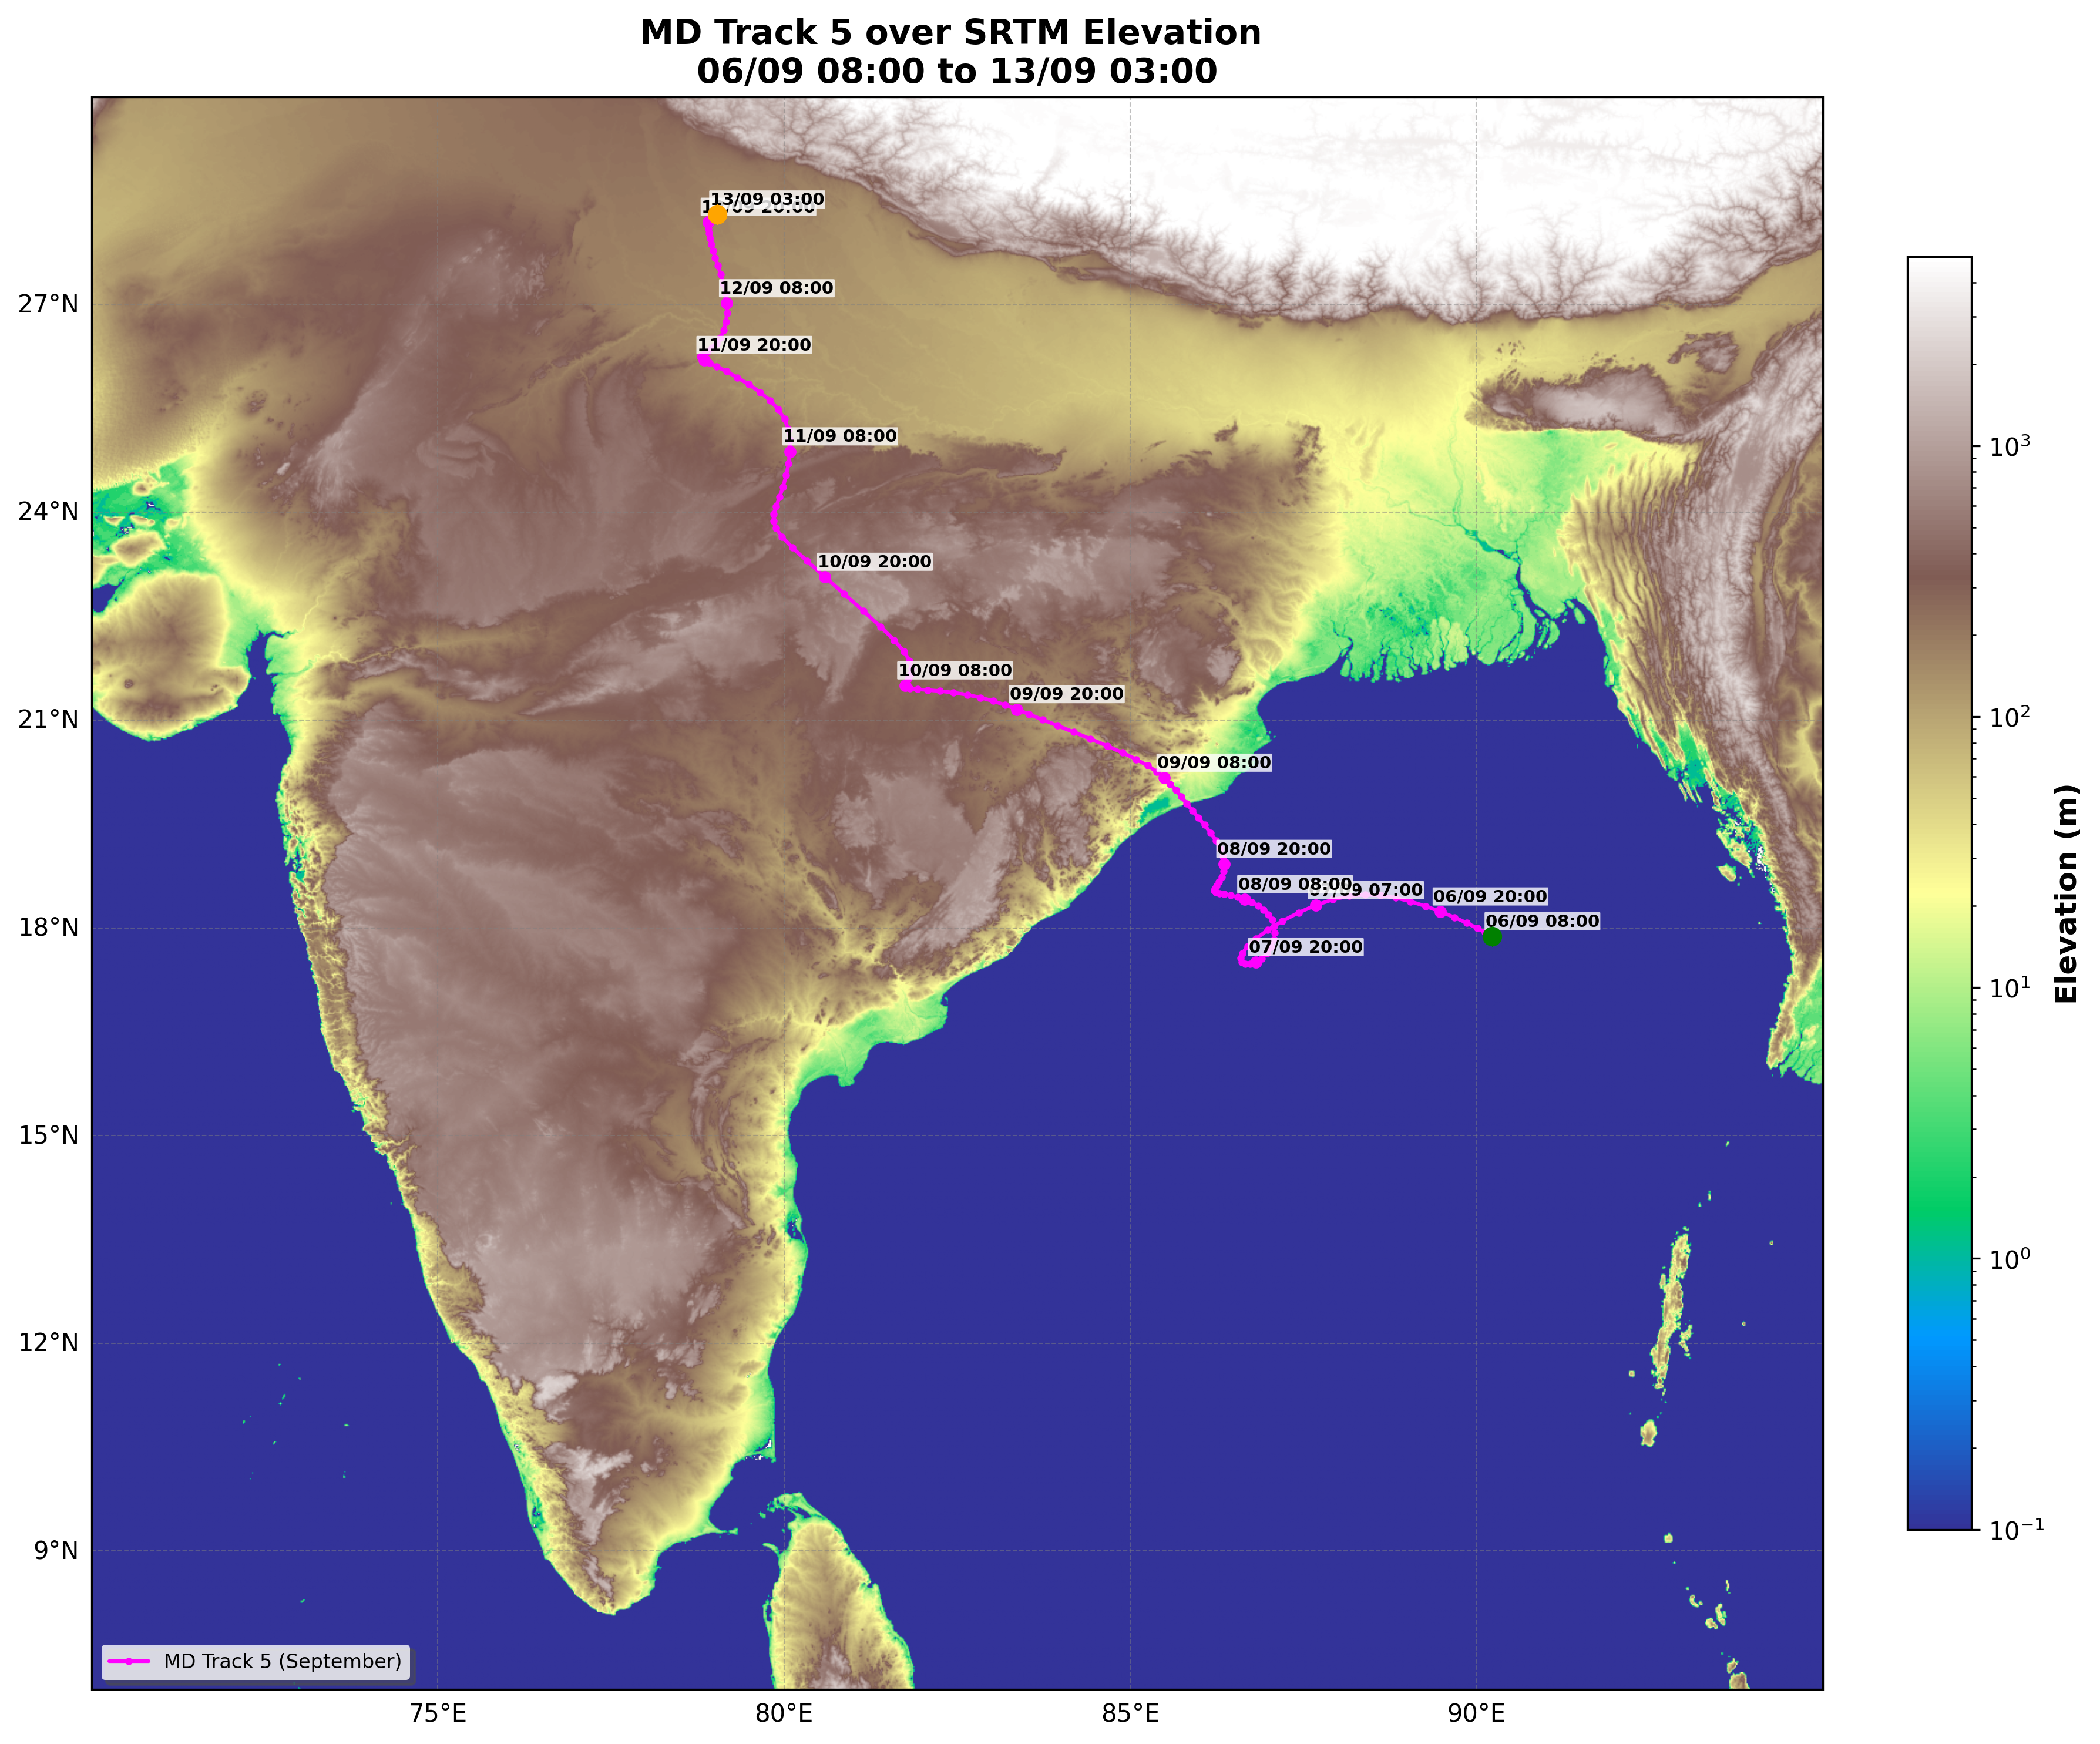
\includegraphics[width=0.85\textwidth]{track_long_elevation_mosaic}
  \caption{BOE-active: Successful terrain crossing and leeward maintenance.}
  \label{fig:long_elevated}
\end{figure}

\begin{figure}[H]
  \centering
  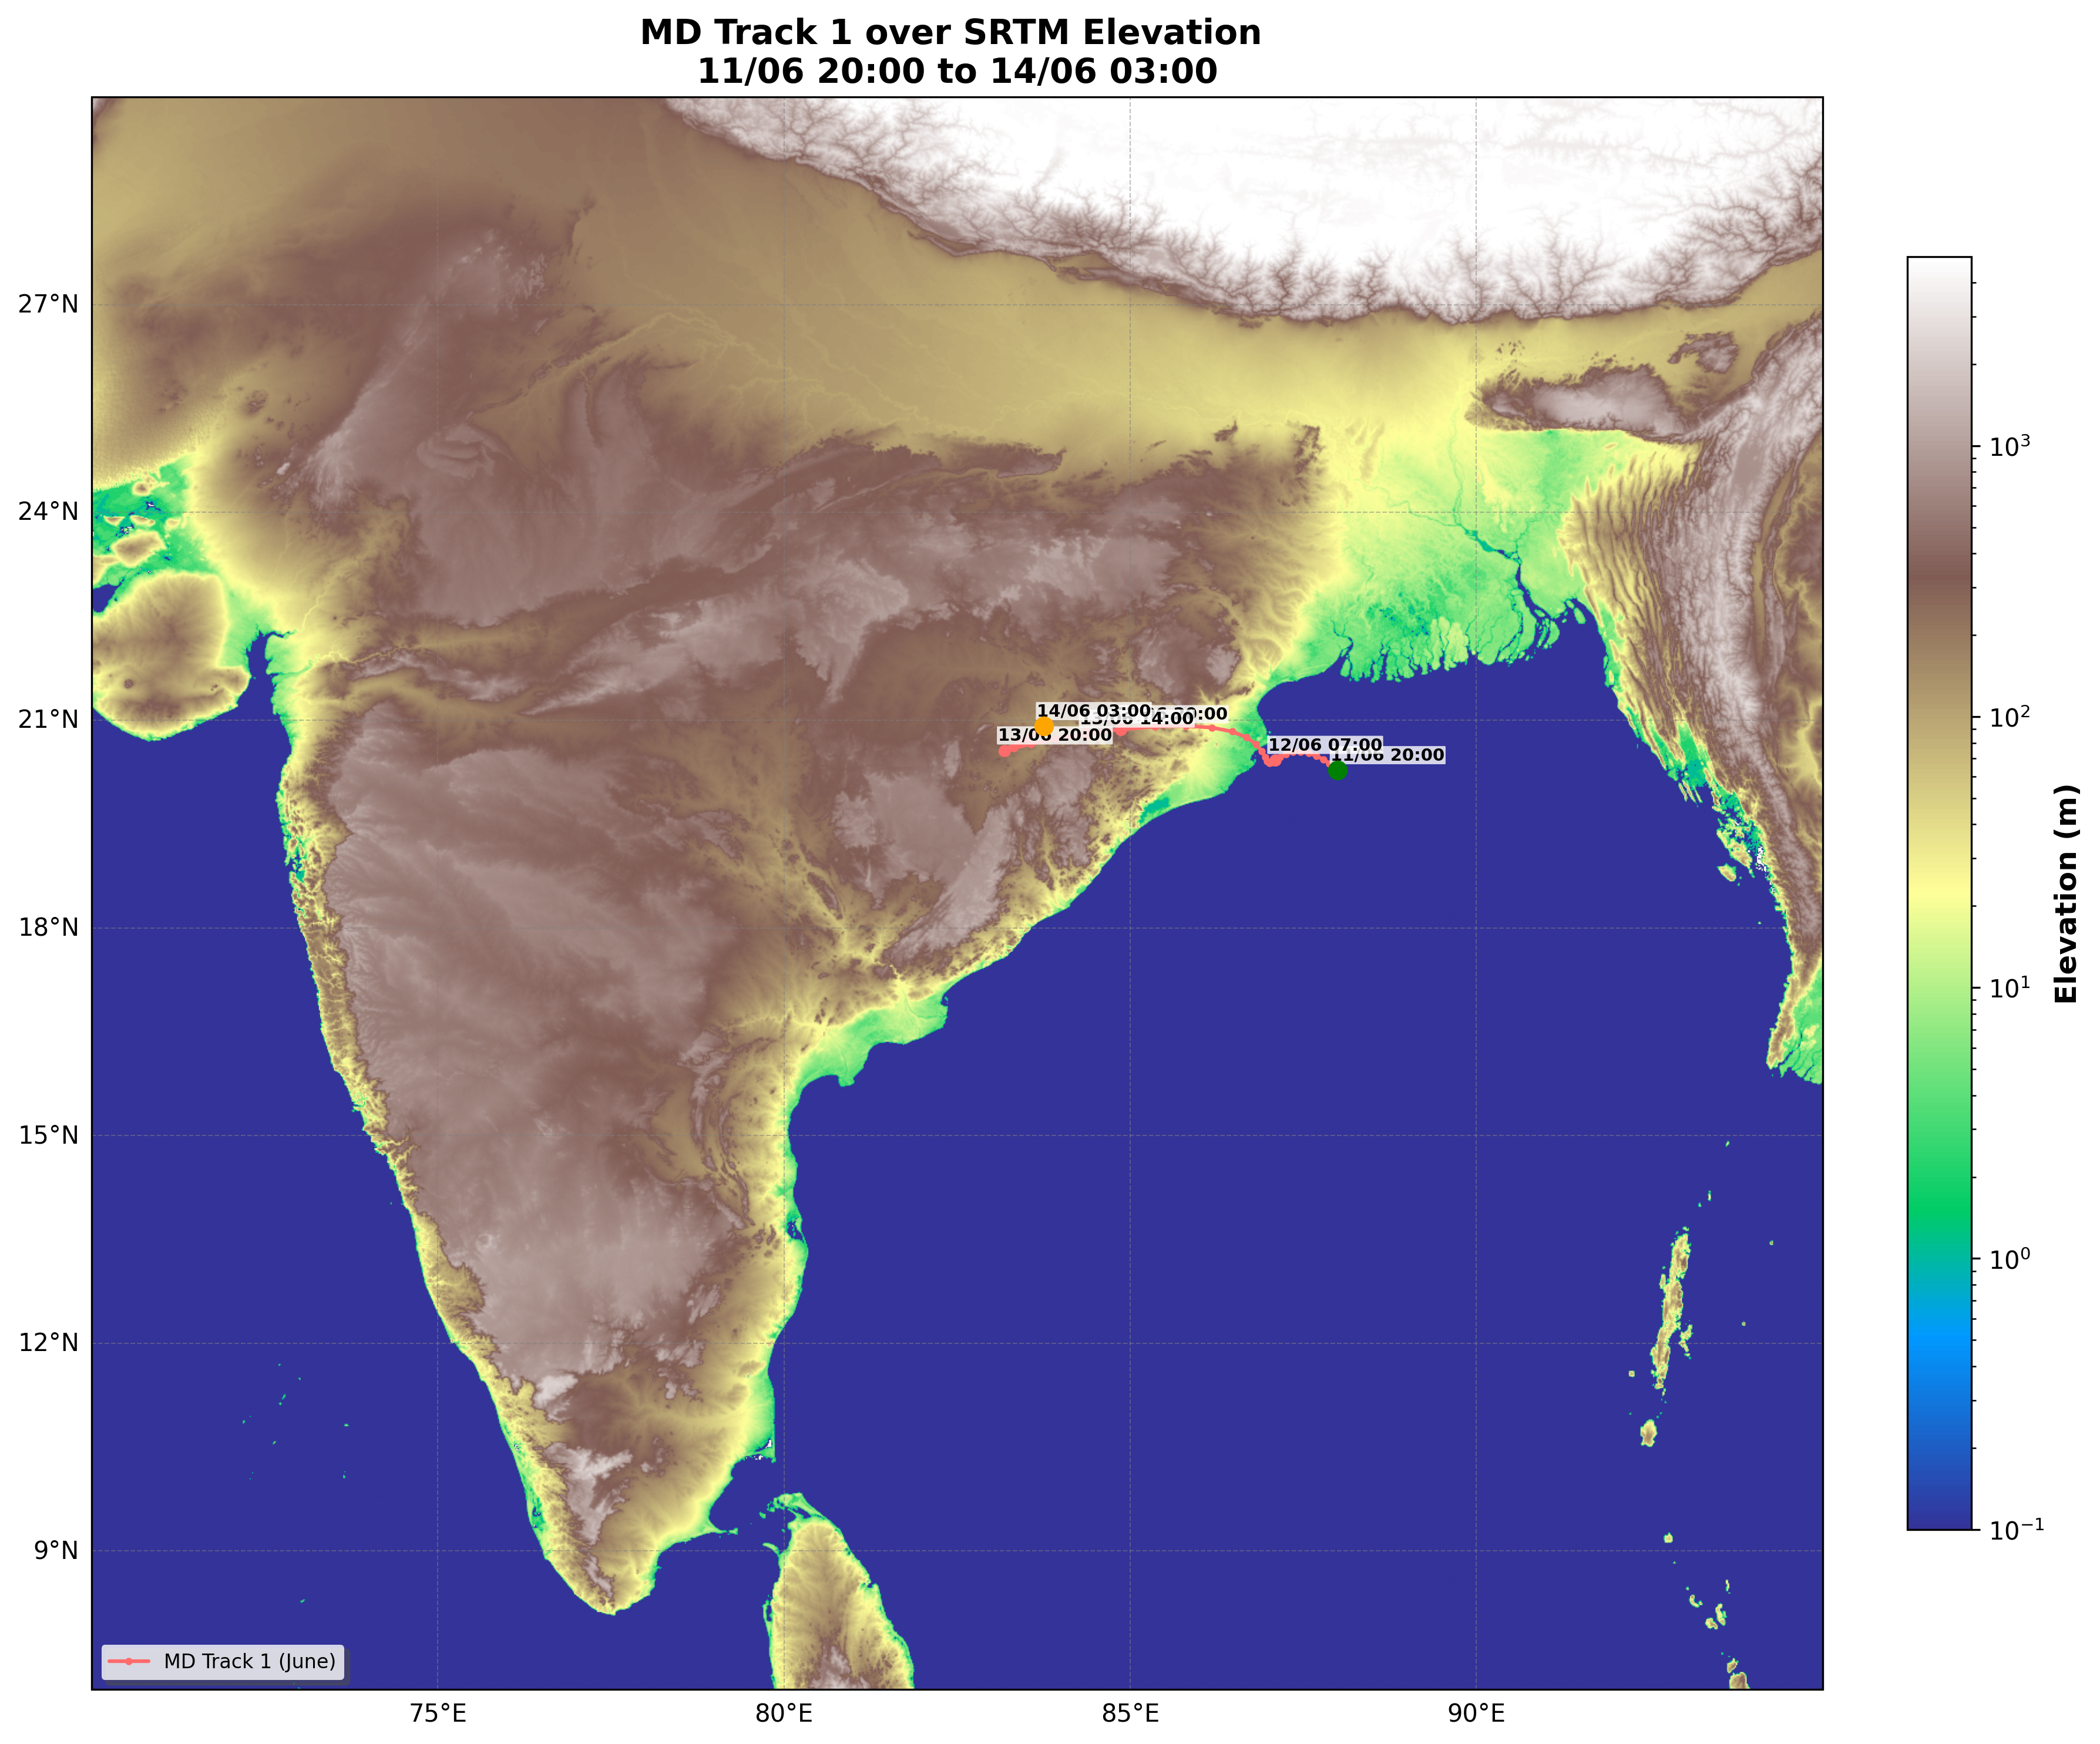
\includegraphics[width=0.85\textwidth]{track_short_elevation_mosaic}
  \caption{Non-BOE: Mechanical dissipation on windward slopes.}
  \label{fig:short_elevated}
\end{figure}

Elevation Mosaic using SRTM data for MD interaction with the Eastern
Ghats. The top panel shows a long-lived track maintaining structural
integrity across high elevation, while the bottom panel illustrates
the typical termination of short-lived systems near the 600\,m contour.

\subsection{Surface Energy Partitioning: LHF and SHF Synchronization}
\label{subsec:ts_hf}

The transition of the surface energy balance at landfall is the
primary determinant of whether a system maintains its oceanic-like
core structure. Figure~\ref{fig:ts_lhf_boe} illustrates the
track-following heat flux evolution for a representative long-lived
(BOE-active) system.

\begin{figure}[H]
  \centering
  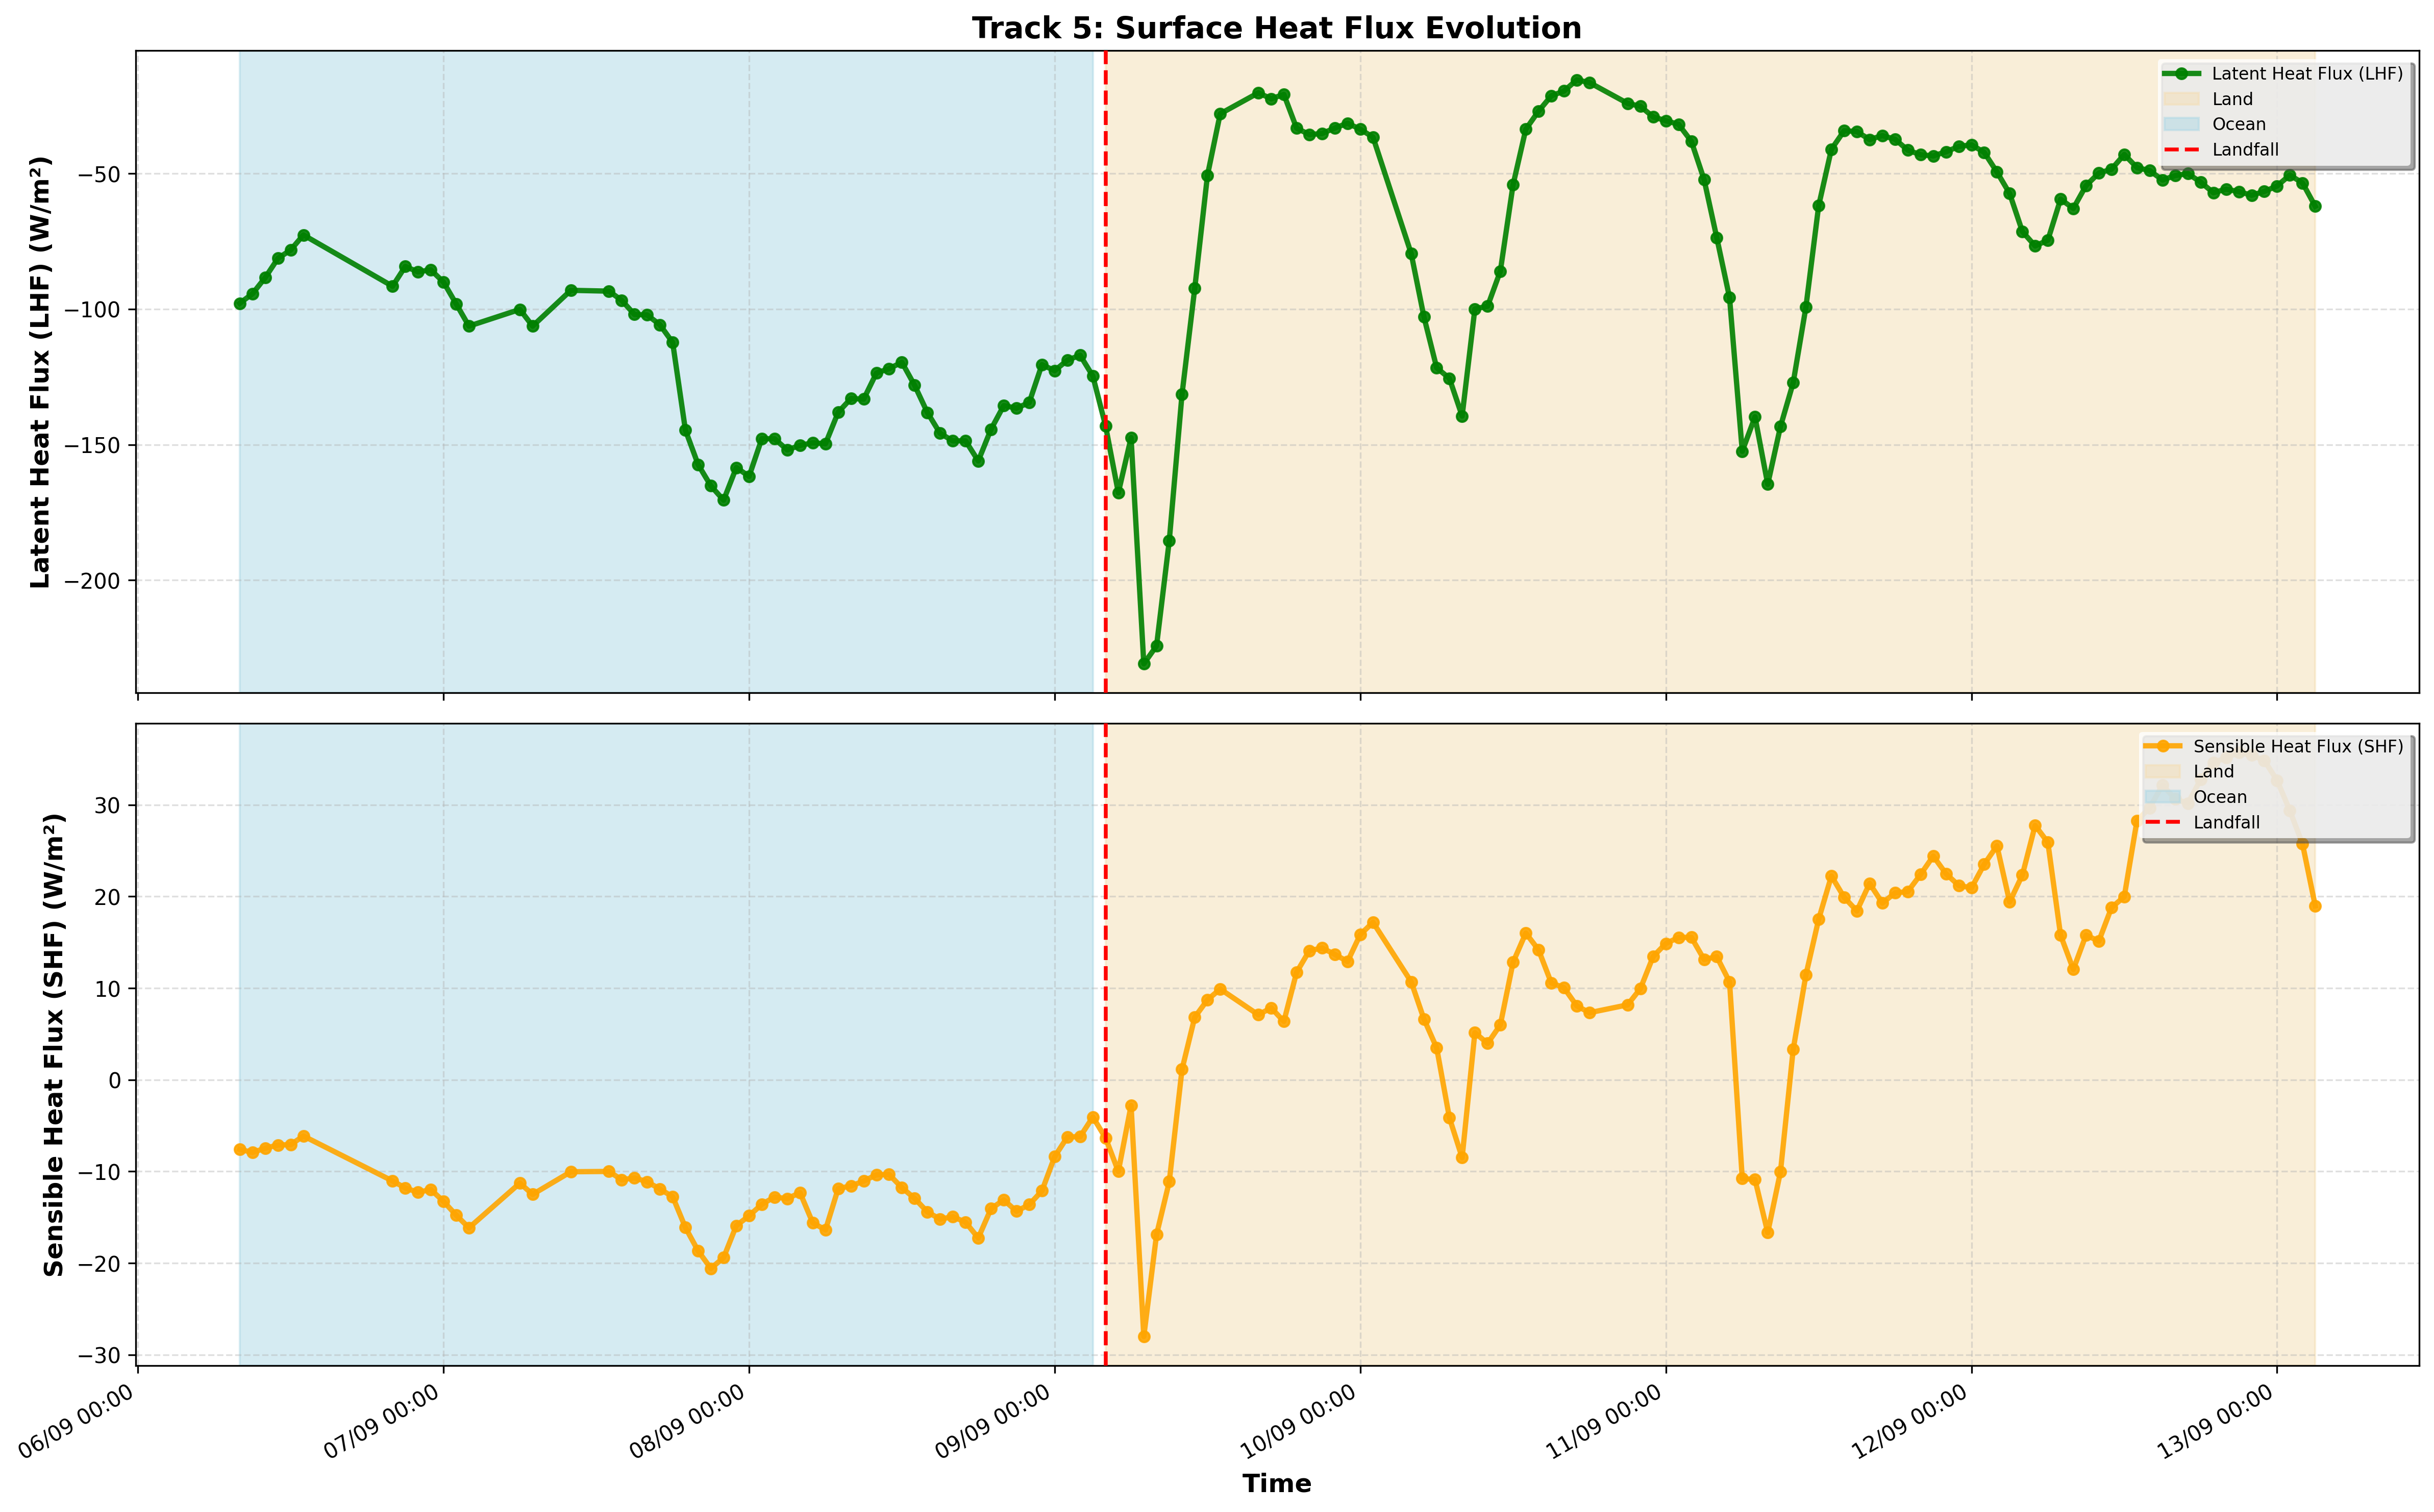
\includegraphics[width=0.9\textwidth]{track_long_HF_time_series}
  \caption{Surface energy fluxes for a long-lived BOE-active MD.
    Continuity of LHF across the landfall boundary and the sustained
  exceedance of the 70\,W\,m$^{-2}$ threshold deep into the land phase.}
  \label{fig:ts_lhf_boe}
\end{figure}

Several thermodynamic features distinguish the BOE-active lifecycle.
\textit{Prior to landfall} ($t < 0$), LHF exceeds
150--200\,W\,m$^{-2}$ while SHF remains near-zero, maintaining the
low-Bowen-ratio state characteristic of the warm Bay of Bengal.
\textit{At landfall} ($t = 0$), the long-lived system exhibits a
resilient energy profile; LHF decreases only modestly and remains
consistently above the 70\,W\,m$^{-2}$ sustaining threshold. This
indicates that the saturated soil acts as an effective surrogate for
the ocean surface. Throughout the land phase ($t > 0$), the system
maintains this high-flux state for over 72~hours, satisfying the
energetic criteria for the Brown Ocean Effect.

In contrast, the short-lived non-BOE population
(Figure~\ref{fig:ts_lhf_nonboe}) displays a fundamental shift in
surface energy partitioning. In these cases, LHF drops below the
critical 70\,W\,m$^{-2}$ threshold within 12--18 hours of landfall.

\begin{figure}[H]
  \centering
  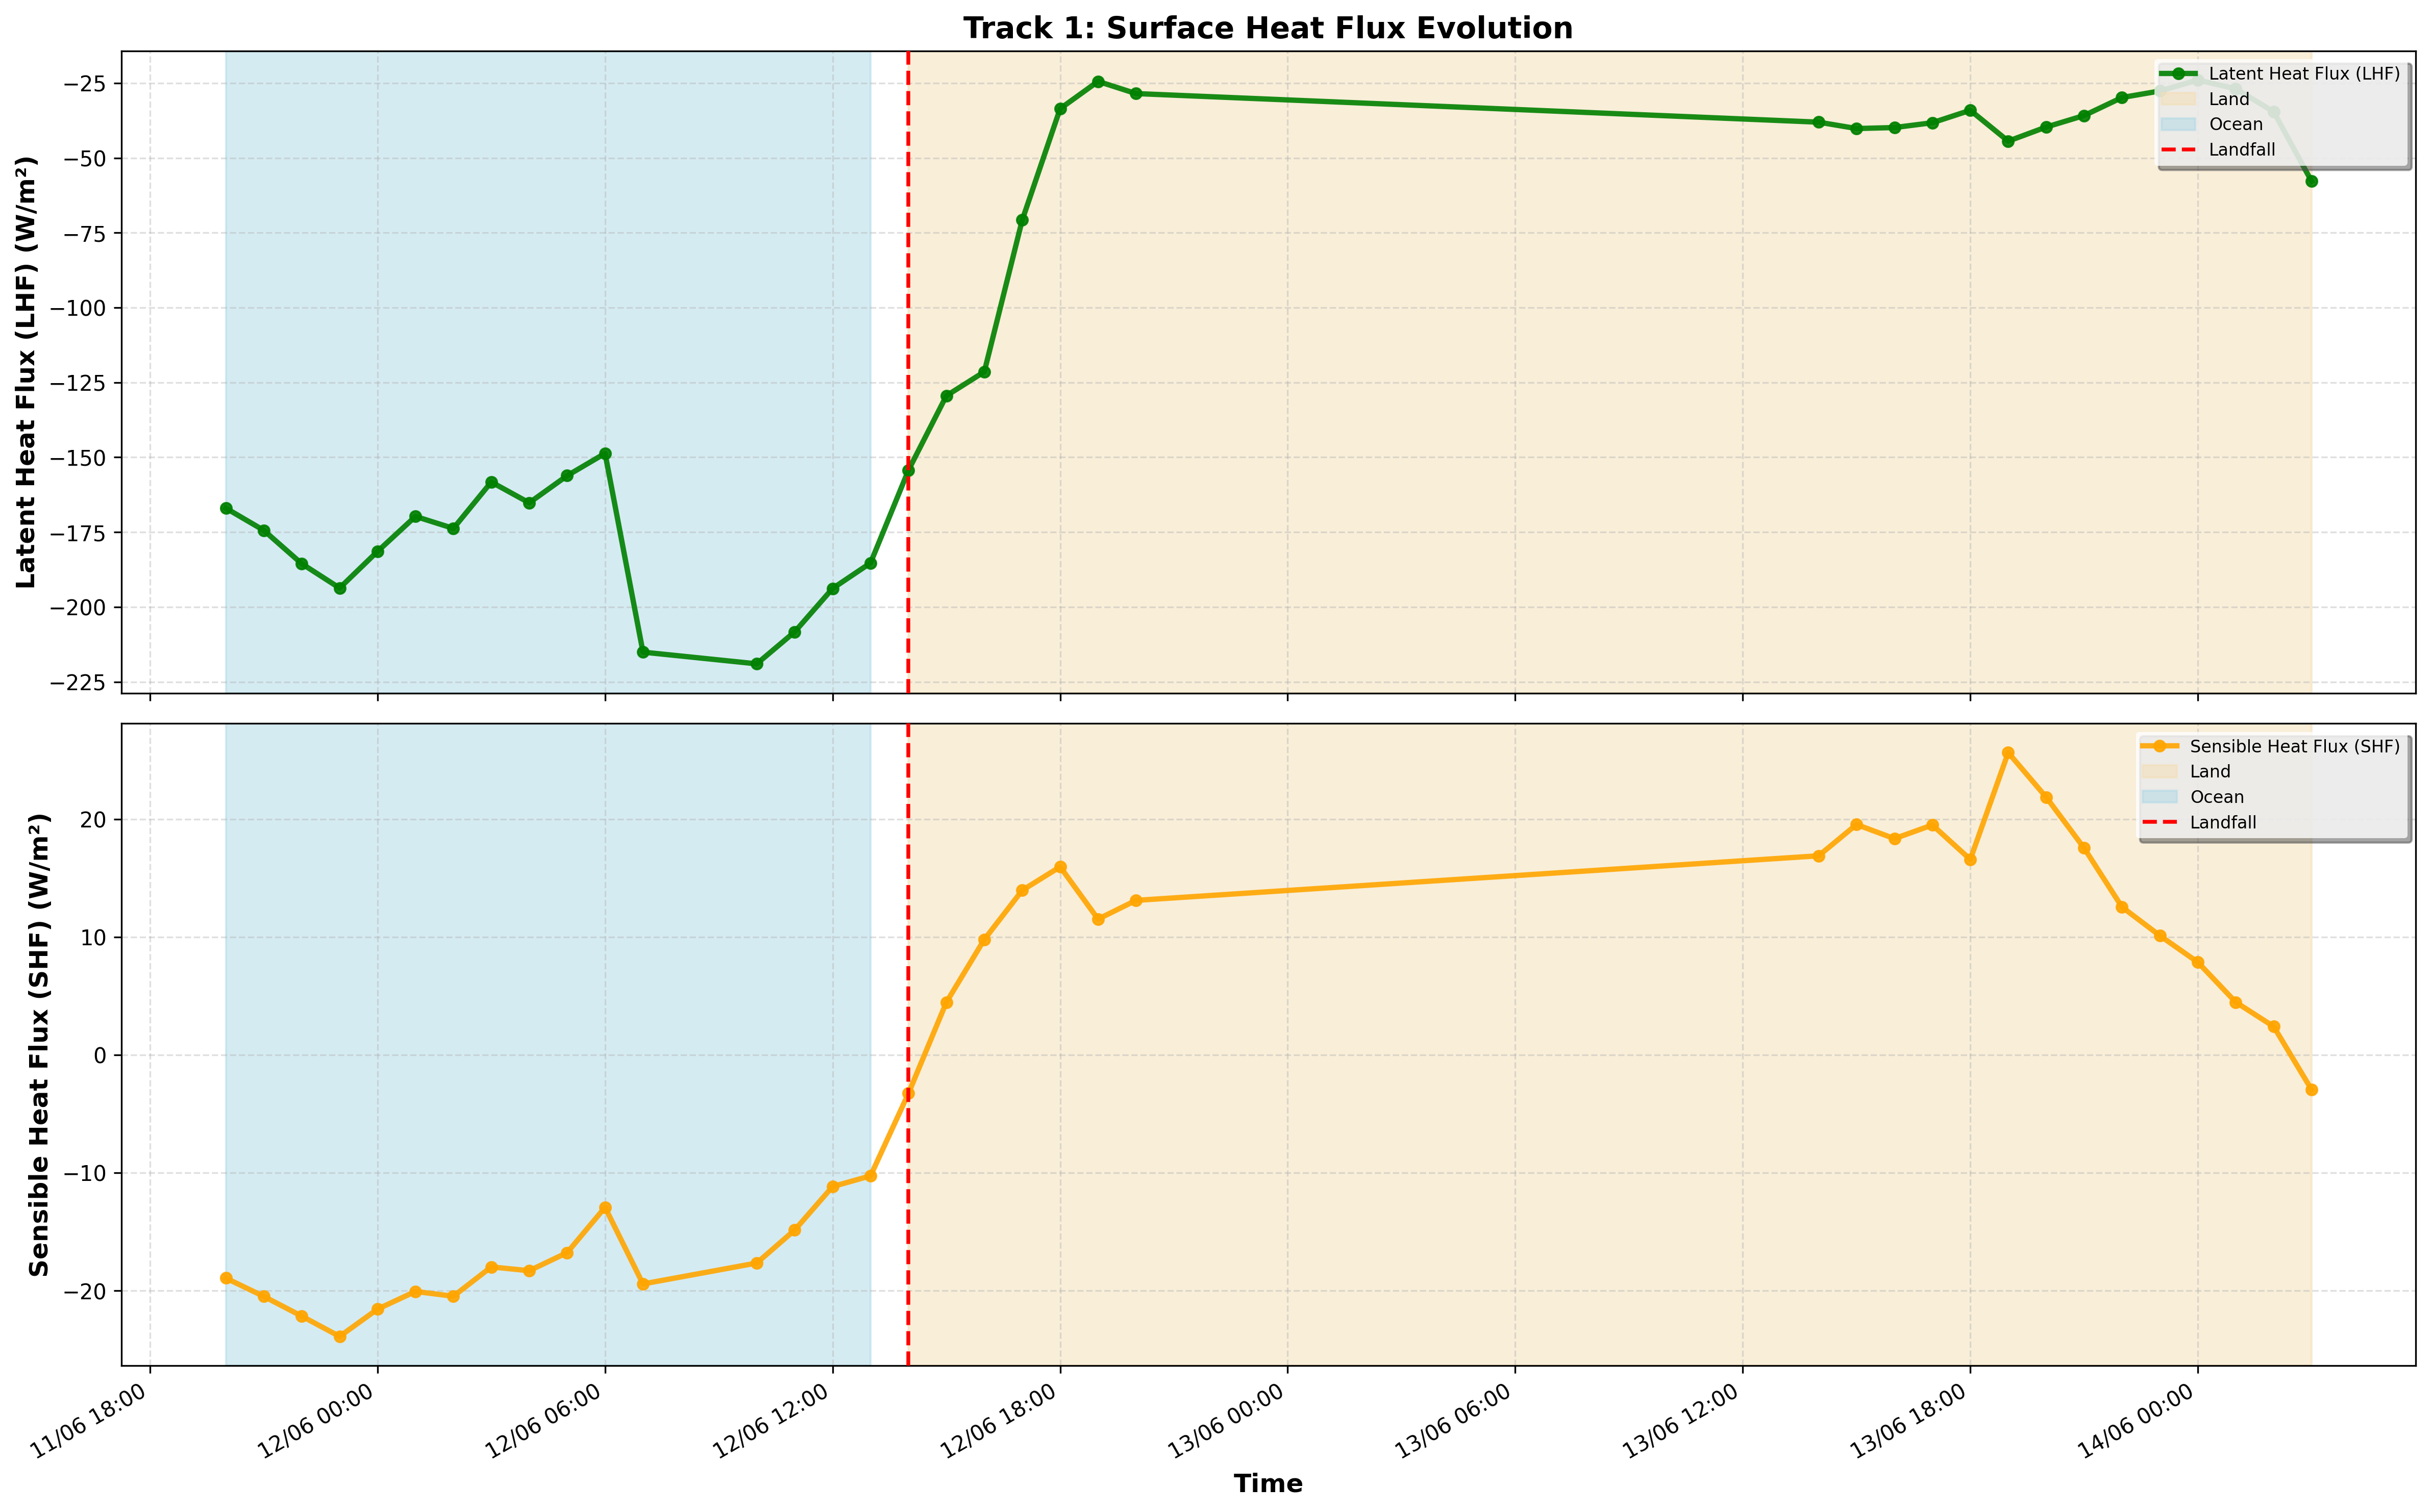
\includegraphics[width=0.9\textwidth]{track_short_HF_time_series}
  \caption{Surface energy fluxes for a short-lived non-BOE MD. The
    rapid collapse of LHF and the corresponding rise in SHF at landfall
  signifies the transition to a water-limited evaporation regime.}
  \label{fig:ts_lhf_nonboe}
\end{figure}

Simultaneously, the SHF in short-lived systems rises sharply to
values exceeding 30--40\,W\,m$^{-2}$. This transition from a latent
dominated to a sensible-dominated regime marks the shift from an
energy-limited to a water-limited surface \autocite{seneviratne2010investigating}.
Physically, this means the surface energy is no longer being utilized
to recycle moisture into the MD's core, but is instead heating the
boundary layer, which encourages dry-air entrainment and triggers
the rapid structural collapse observed in Section~\ref{subsec:hovmoller_tp}.

\subsection{Feedback: The Precipitation-Soil Moisture Loop}
\label{subsec:ts_sm_tp}

The integration of heat flux diagnostics with the temporal evolution
of moisture confirms the existence of a closed-loop feedback in
BOE-active systems. While the Hovm\"{o}ller analysis captures the
radial contraction of the MD, the track-following time-series
(Figures~\ref{fig:long_ts_sm_tp} and \ref{fig:short_ts_sm_tp})
reveals the temporal synchronization required for inland maintenance.

\subsubsection*{Self-Wetting Dynamics in BOE-Active Systems}

Figure~\ref{fig:long_ts_sm_tp} illustrates the co-evolution of
\texttt{swvl1} and total precipitation (\texttt{TP}) for a
representative long-lived MD. Three temporal features define the BOE
maintenance phase:
\begin{enumerate}
  \item \textbf{Pre-conditioned Landfall ($t=0$):} The system
    encounters antecedent soil moisture levels already $\geq
    0.35$\,m$^3$\,m$^{-3}$. This high initial state prevents the
    standard surface energy collapse associated with dry-landfall.
  \item \textbf{The Intensive Wetting Phase ($0 < t < 36$\,h):}
    Post-landfall, \texttt{swvl1} rises progressively toward field
    capacity ($\sim 0.46$\,m$^3$\,m$^{-3}$). This rise is driven by
    the MD's own inner-core precipitation, which remains sustained
    around 4\,mm\,h$^{-1}$.
  \item \textbf{Phase Synchronization:} The simultaneous maintenance
    of heavy precipitation while \texttt{swvl1} approaches saturation
    confirms a positive feedback loop. The storm's rainfall sustains
    the soil reservoir, which in turn fuels the LHF
    ($>70$\,W\,m$^{-2}$) necessary to drive subsequent deep convection.
\end{enumerate}

\begin{figure}[H]
  \centering
  \includegraphics[width=0.98\textwidth]{track_long_tp-swvl1_time_series}
  \caption[Co-evolution of Soil moisture (\texttt{SWVL1}) and Total
  precipitation (\texttt{TP}), BOE-active MD]{Track-following Soil
    moisture \texttt{SWVL1} and Total precipitation (\texttt{TP}) for a
    long-lived MD. The sustained precipitation concurrent with rising
  soil moisture indicates the establishment of a self-wetting feedback loop.}
  \label{fig:long_ts_sm_tp}
\end{figure}

\subsubsection*{Feedback Failure in Short-Lived Systems}

For comparison, the non-BOE system (Figure~\ref{fig:short_ts_sm_tp})
exhibits a failure to establish this feedback. Although the system
may produce an initial burst of precipitation at landfall, the lack
of pre-conditioned soil leads to rapid surface desiccation. Without
the moisted land surface provided by high antecedent soil moisture, the
LHF collapses (as seen in Section~\ref{subsec:ts_hf}), causing the
precipitation to cease before the soil can reach a sustaining level
of saturation. This confirms that the BOE is a threshold-gated
mechanism; if the self-wetting loop is not activated within the first
24 hours of landfall, the system inevitably undergoes structural decay.

\begin{figure}[H]
  \centering
  \includegraphics[width=0.98\textwidth]{track_short_tp-swvl1_time_series}
  \caption[Co-evolution of Soil moisture (\texttt{SWVL1}) and
  precipitation (\texttt{TP}), Non-BOE MD]{Track-following
    \texttt{swvl1} and precipitation for a short-lived MD. The rapid
    decline in precipitation at $t \approx 18$\,h prevents the soil
    from reaching field capacity, resulting in the dissipation of the
  surface energy reservoir.}
  \label{fig:short_ts_sm_tp}
\end{figure}

% \subsection{Bowen Ratio: Quantifying Evaporation}
% \label{subsec:ts_bowen}
%
% From Figure~\ref{fig:ts_bowen}, the Bowen ratio trajectory isolates
% the transition most clearly. Over the ocean ($t < 0$), both
% long-lived and short-lived categories show $\beta \approx
% 0.2$-$0.3$, the characteristic low Bowen ratio of a moisture-rich
% surface. At landfall, the divergence between the two populations is
% immediate and quantitatively large. For BOE candidates, $\beta$
% rises only to $\approx 0.4$-$0.5$, confirming that the surface
% remains in the energy-limited evaporation throughout the land
% phase: evaporation is limited not by water supply but by the
% available radiative energy. For non-BOE systems, $\beta$ rises
% steeply, exceeding 1.0 within \textbf{[T\_beta1]}\,hours of
% landfall, meaning sensible heating has overtaken latent heating. A
% $\beta > 1.0$ implies the surface is actively heating the boundary
% layer while providing insufficient moisture flux to sustain
% convective instability-a state incompatible with continued MD organisation.
%
% %%  FIGURE: Bowen ratio comparison
% %%  SOURCE: output_YYYY/track_N/time_series/track_N_bowen_ratio.png
% %%  Overlay BOTH long-lived (orange) and short-lived (blue) on same axes.
% %%  Add reference lines at beta = 0.3 (oceanic value) and beta = 1.0 (parity).
% \begin{figure}[H]
%   \centering
%   %% >> INSERT FIGURE: overlay of BOE-candidate and non-BOE Bowen
% ratio plots <<
%   \fbox{\rule{0pt}{6cm}\rule{0.85\textwidth}{0pt}}
%   % \includegraphics[width=0.85\textwidth]{bowen_ratio_comparison}
%   \caption[Track-following Bowen ratio time series]{Bowen ratio
%     ($\beta = Q_H/Q_E$)
%     for long-lived BOE-candidate (orange) and short-lived non-BOE (blue) MDs.
%     Reference lines at $\beta = 0.3$ (oceanic value) and $\beta =
% 1.0$ (LHF/SHF
%     parity). The divergence after $t = 0$ reflects fundamentally
%     different post-landfall
%   surface energy regimes.}
%   \label{fig:ts_bowen}
% \end{figure}

\subsection{Translational Speed: Terrain Deceleration and BOE Recovery}
\label{subsec:ts_speed}

The interaction between the MD core and the complex orography of the
Eastern Ghats is most clearly visible in the evolution of
translational speed ($V_t$). As shown in the elevation-speed maps
(Figures~\ref{fig:track_long_speed_map} and
\ref{fig:track_short_speed_map}), elevation acts as a mechanical sink
for the system's kinetic energy.

\textit{Over the ocean}, MDs translate at a steady mean speed of
6\,m\,s$^{-1}$. However, as the systems encounter the 200-1000\,m
elevation gradient of the Eastern Ghats, both MDs undergo significant
deceleration. This is consistent with increased surface roughness and
mechanical flow blocking \autocite{houze1994}, which reduces the
low-level momentum of the vortex.

The critical divergence occurs west of the main terrain crest.
Long-lived (BOE-active) systems exhibit a clear leeward speed
recovery; as elevation drops below 200\,m, the speed returns to
approximately 5\,m\,s$^{-1}$. This suggests that the sustained
surface LHF (the BOE engine) maintains the low-level pressure
gradient force required to drive the system forward.

Conversely, short-lived systems fail to overcome the mechanical drag
by elevated land. In Figure~\ref{fig:track_short_speed_map}, these
tracks often show a stalling behavior or a slight recurvature before
dissipating. Without the thermodynamic replenishment from the soil,
the convective MD vortex structure collapses during the
terrain-crossing phase, leading to a permanent loss of translational
momentum and subsequent track termination.

\begin{figure}[H]
  \centering
  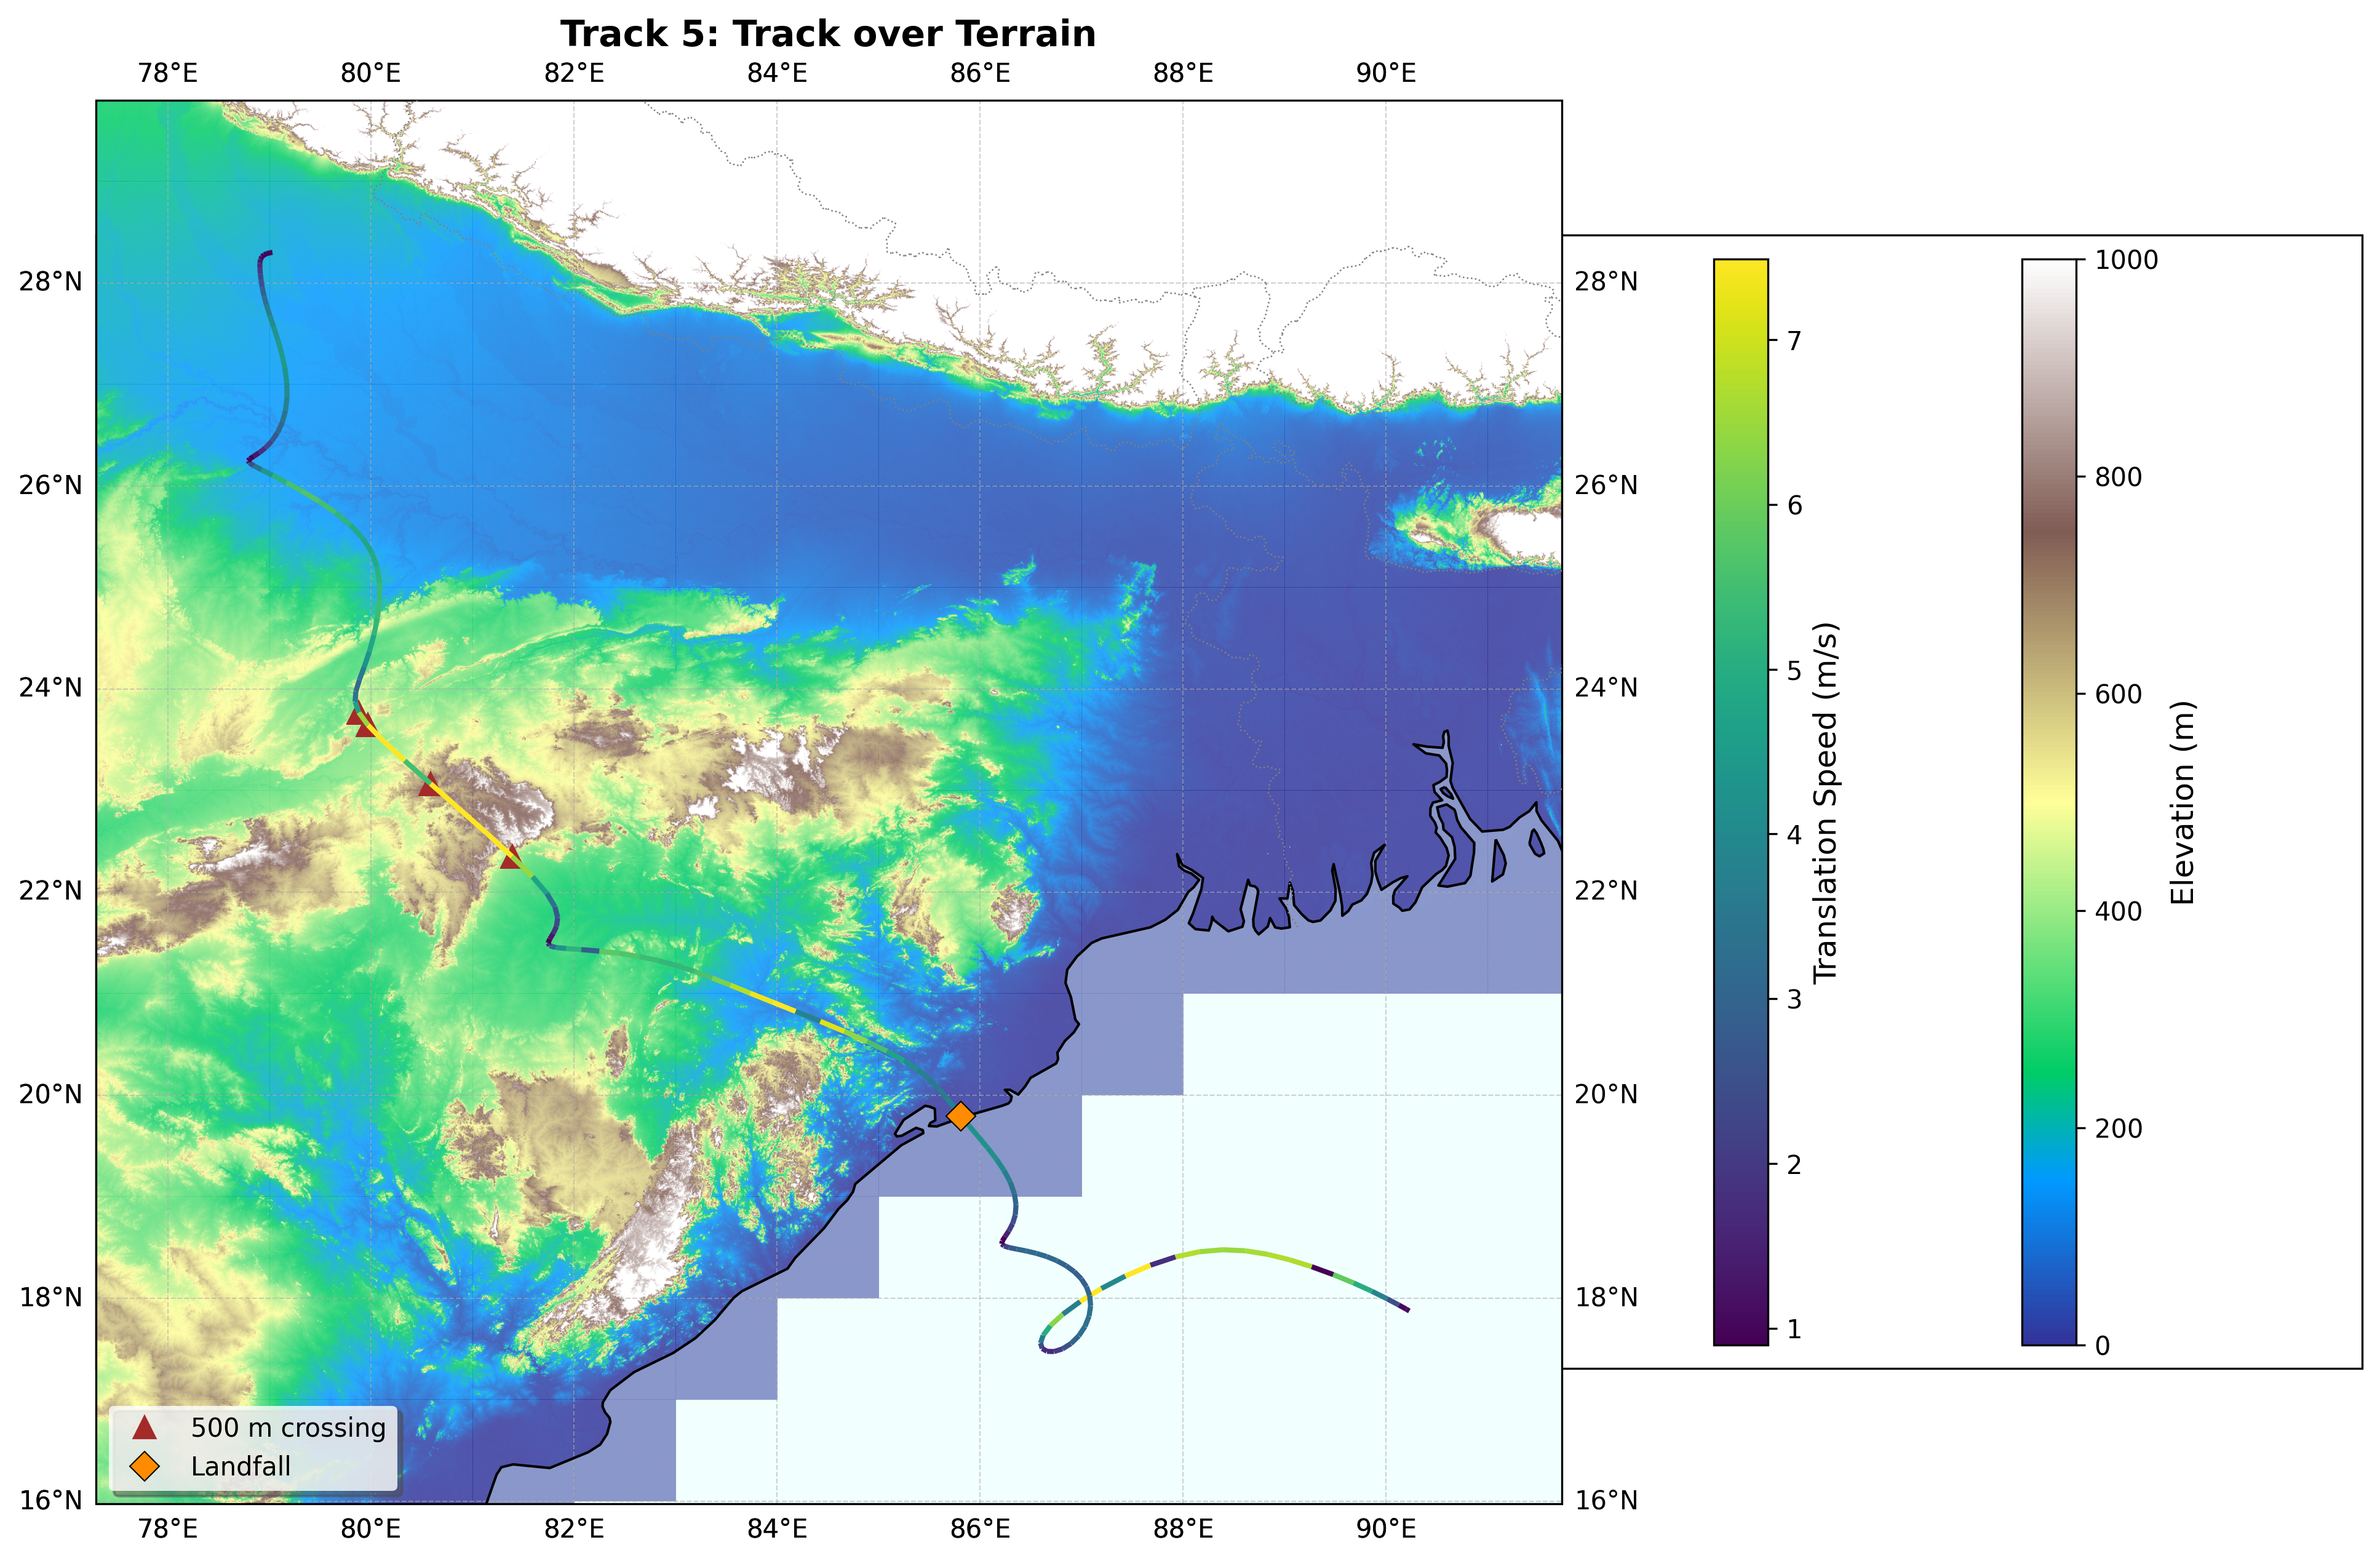
\includegraphics[width=0.86\textwidth]{track_long_elevation_speed_map}
  \caption{BOE-active: Speed recovery following the crossing of the
  600\,m contour.}
  \label{fig:track_long_speed_map}
\end{figure}

\begin{figure}[H]
  \centering
  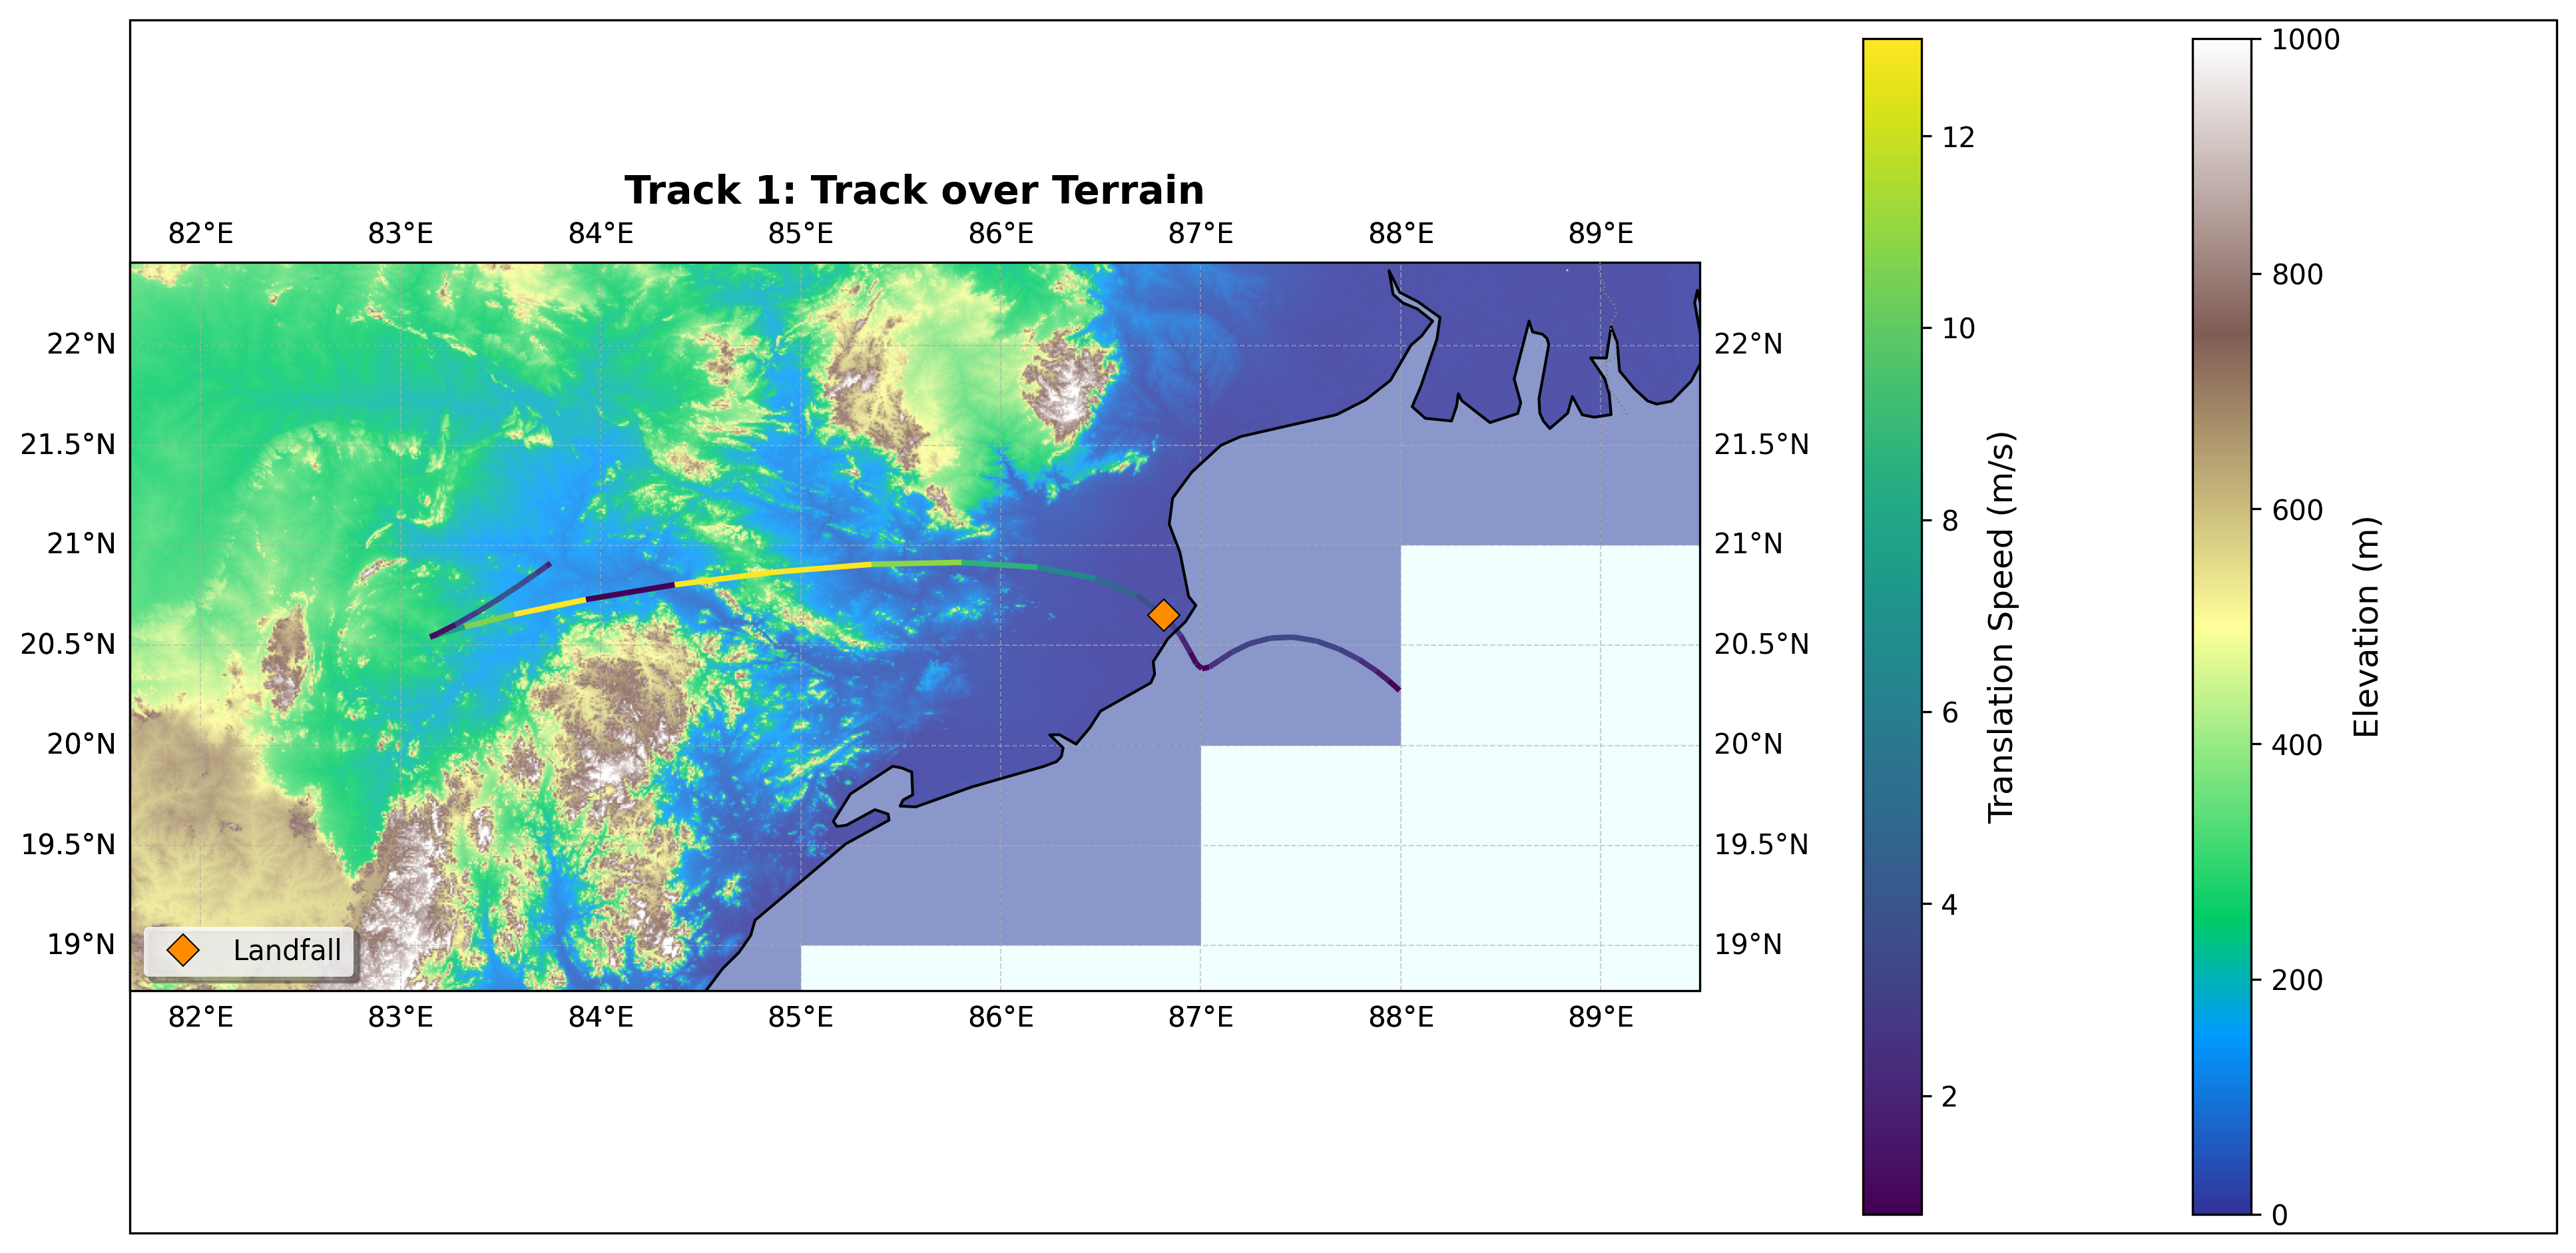
\includegraphics[width=0.86\textwidth]{track_short_elevation_speed_map}
  \caption{Non-BOE: Sustained deceleration and track termination
  upon terrain encounter.}
  \label{fig:track_short_speed_map}
\end{figure}

Spatial evolution of MD translational speed overlaid on SRTM
elevation. While both systems decelerate upon landfall, the
long-lived system exhibits a post-terrain re-acceleration, signaling
a replenishment of vortex strength via the BOE.

\section{Synthesis: The BOE as a Diagnostic Mechanism}
\label{subsec:results_synthesis}

The results presented from the azimuthal Hovm\"{o}ller
(\ref{sec:results_hovmoller}) and terrain analyses
(\ref{sec:results_elevation}) demonstrate that the Brown Ocean Effect
is not a predictive coincidence, but a synchronized physical state.
In every confirmed long-lived event, four independent observational
signals converge at landfall:
\begin{enumerate}
  \item \textbf{Inward Contraction:} Precipitation maximum shifts
    from a broad maritime footprint to a concentrated inner-core
    ($<100$\,km) structure.
  \item \textbf{Self-Wetting Persistence:} Core rainfall maintains a
    saturated soil reservoir ($>0.40$\,m$^3$\,m$^{-3}$), preventing the
    surface desiccation that usually follows landfall.
  \item \textbf{Oceanic-Scale Fluxes:} Land-phase Latent Heat Flux
    remains above the sustaining threshold ($>70$\,W\,m$^{-2}$),
    effectively mimicking the energy environment of the Bay of Bengal.
  \item \textbf{Thermodynamic Stability:} The partitioning of energy
    into evaporation rather than sensible heating (low Bowen Ratio)
    preserves a cool, moist boundary layer and a low Lifting
    Condensation Level (LCL).
\end{enumerate}

The presence of this synchronized signature explains the ``Predictive
Paradox'' of MD longevity. While mechanical factors like the Eastern
Ghats modulate the translational speed of all systems, only
BOE-active systems exhibit a leeward speed recovery. This confirms
that the thermodynamic energy supply provided by land-atmosphere
coupling is the primary determinant of whether a system penetrates
the Indian inland or dissipates near coast.

% \subsection{Windward-Leeward Dew-Point Depression Asymmetry at the Ghats}
% \label{subsec:ts_dpd_asymmetry}
%
% \yellownote{TODO: Update values}
% From Figure~\ref{fig:ts_dpd_asymmetry}, the windward (eastern) sector
% DPD remains $<3$\,K throughout the terrain-crossing period, as
% expected: forced ascent on the eastern Ghats slopes sustains
% saturated conditions in the windward boundary layer.
% The leeward (western) sector DPD increases during Ghats crossing in
% both BOE-candidate and non-BOE systems, reflecting föhn-induced
% warming and drying.
% However, the leeward DPD increase is substantially smaller in
% BOE-candidate systems (\textbf{[DDPD\_BOE]}\,K vs
% \textbf{[DDPD\_nonBOE]}\,K for non-BOE systems).
% This difference indicates that surface evapotranspiration from the
% wet leeward soil is actively counteracting the orographic drying,
% partially re-moistening the leeward boundary layer and preserving
% convective potential on the leeward side.
% This mechanism-the BOE offsetting Ghats-induced leeward
% drying-provides the specific boundary-layer pathway through which the
% BOE allows MDs to survive terrain crossing.
%
% %%  FIGURE: Windward-leeward DPD asymmetry
% \begin{figure}[H]
%   \centering
%   \fbox{\rule{0pt}{6cm}\rule{0.85\textwidth}{0pt}}
%   % \includegraphics[width=0.85\textwidth]{dpd_windward_leeward}
%   \caption[Windward-leeward DPD asymmetry during Ghats
% crossing]{DPD (K) for the windward and leeward sectors during
% Eastern Ghats crossing. Smaller leeward DPD increase in
% BOE-candidate systems reflects BOE evapotranspiration counteracting
% orographic drying.}
%   \label{fig:ts_dpd_asymmetry}
% \end{figure}

\section{The Eastern Ghats Filtering Effect: Identification of Survivors}
\label{sec:ghats_filtering}

While the majority of Monsoon Depressions (MDs) dissipate within 48
hours of interacting with the rugged topography of the Eastern Ghats,
a distinct subset of systems exhibits anomalous longevity.
Figure~\ref{fig:ghats_survivors_map} illustrates this spatial
dichotomy. The background (gray tracks) shows the climatological
termination of MDs along the coast, effectively treating the Ghats as
a topographic 'wall'.

However, four specific systems---2005 (T6), 2017 (T4), 2021 (T5), and
2024 (T4)---demonstrate the 'filter' effect, maintaining structural
integrity and MD-level intensity despite crossing high-relief regions.

\begin{figure}[H]
  \centering
  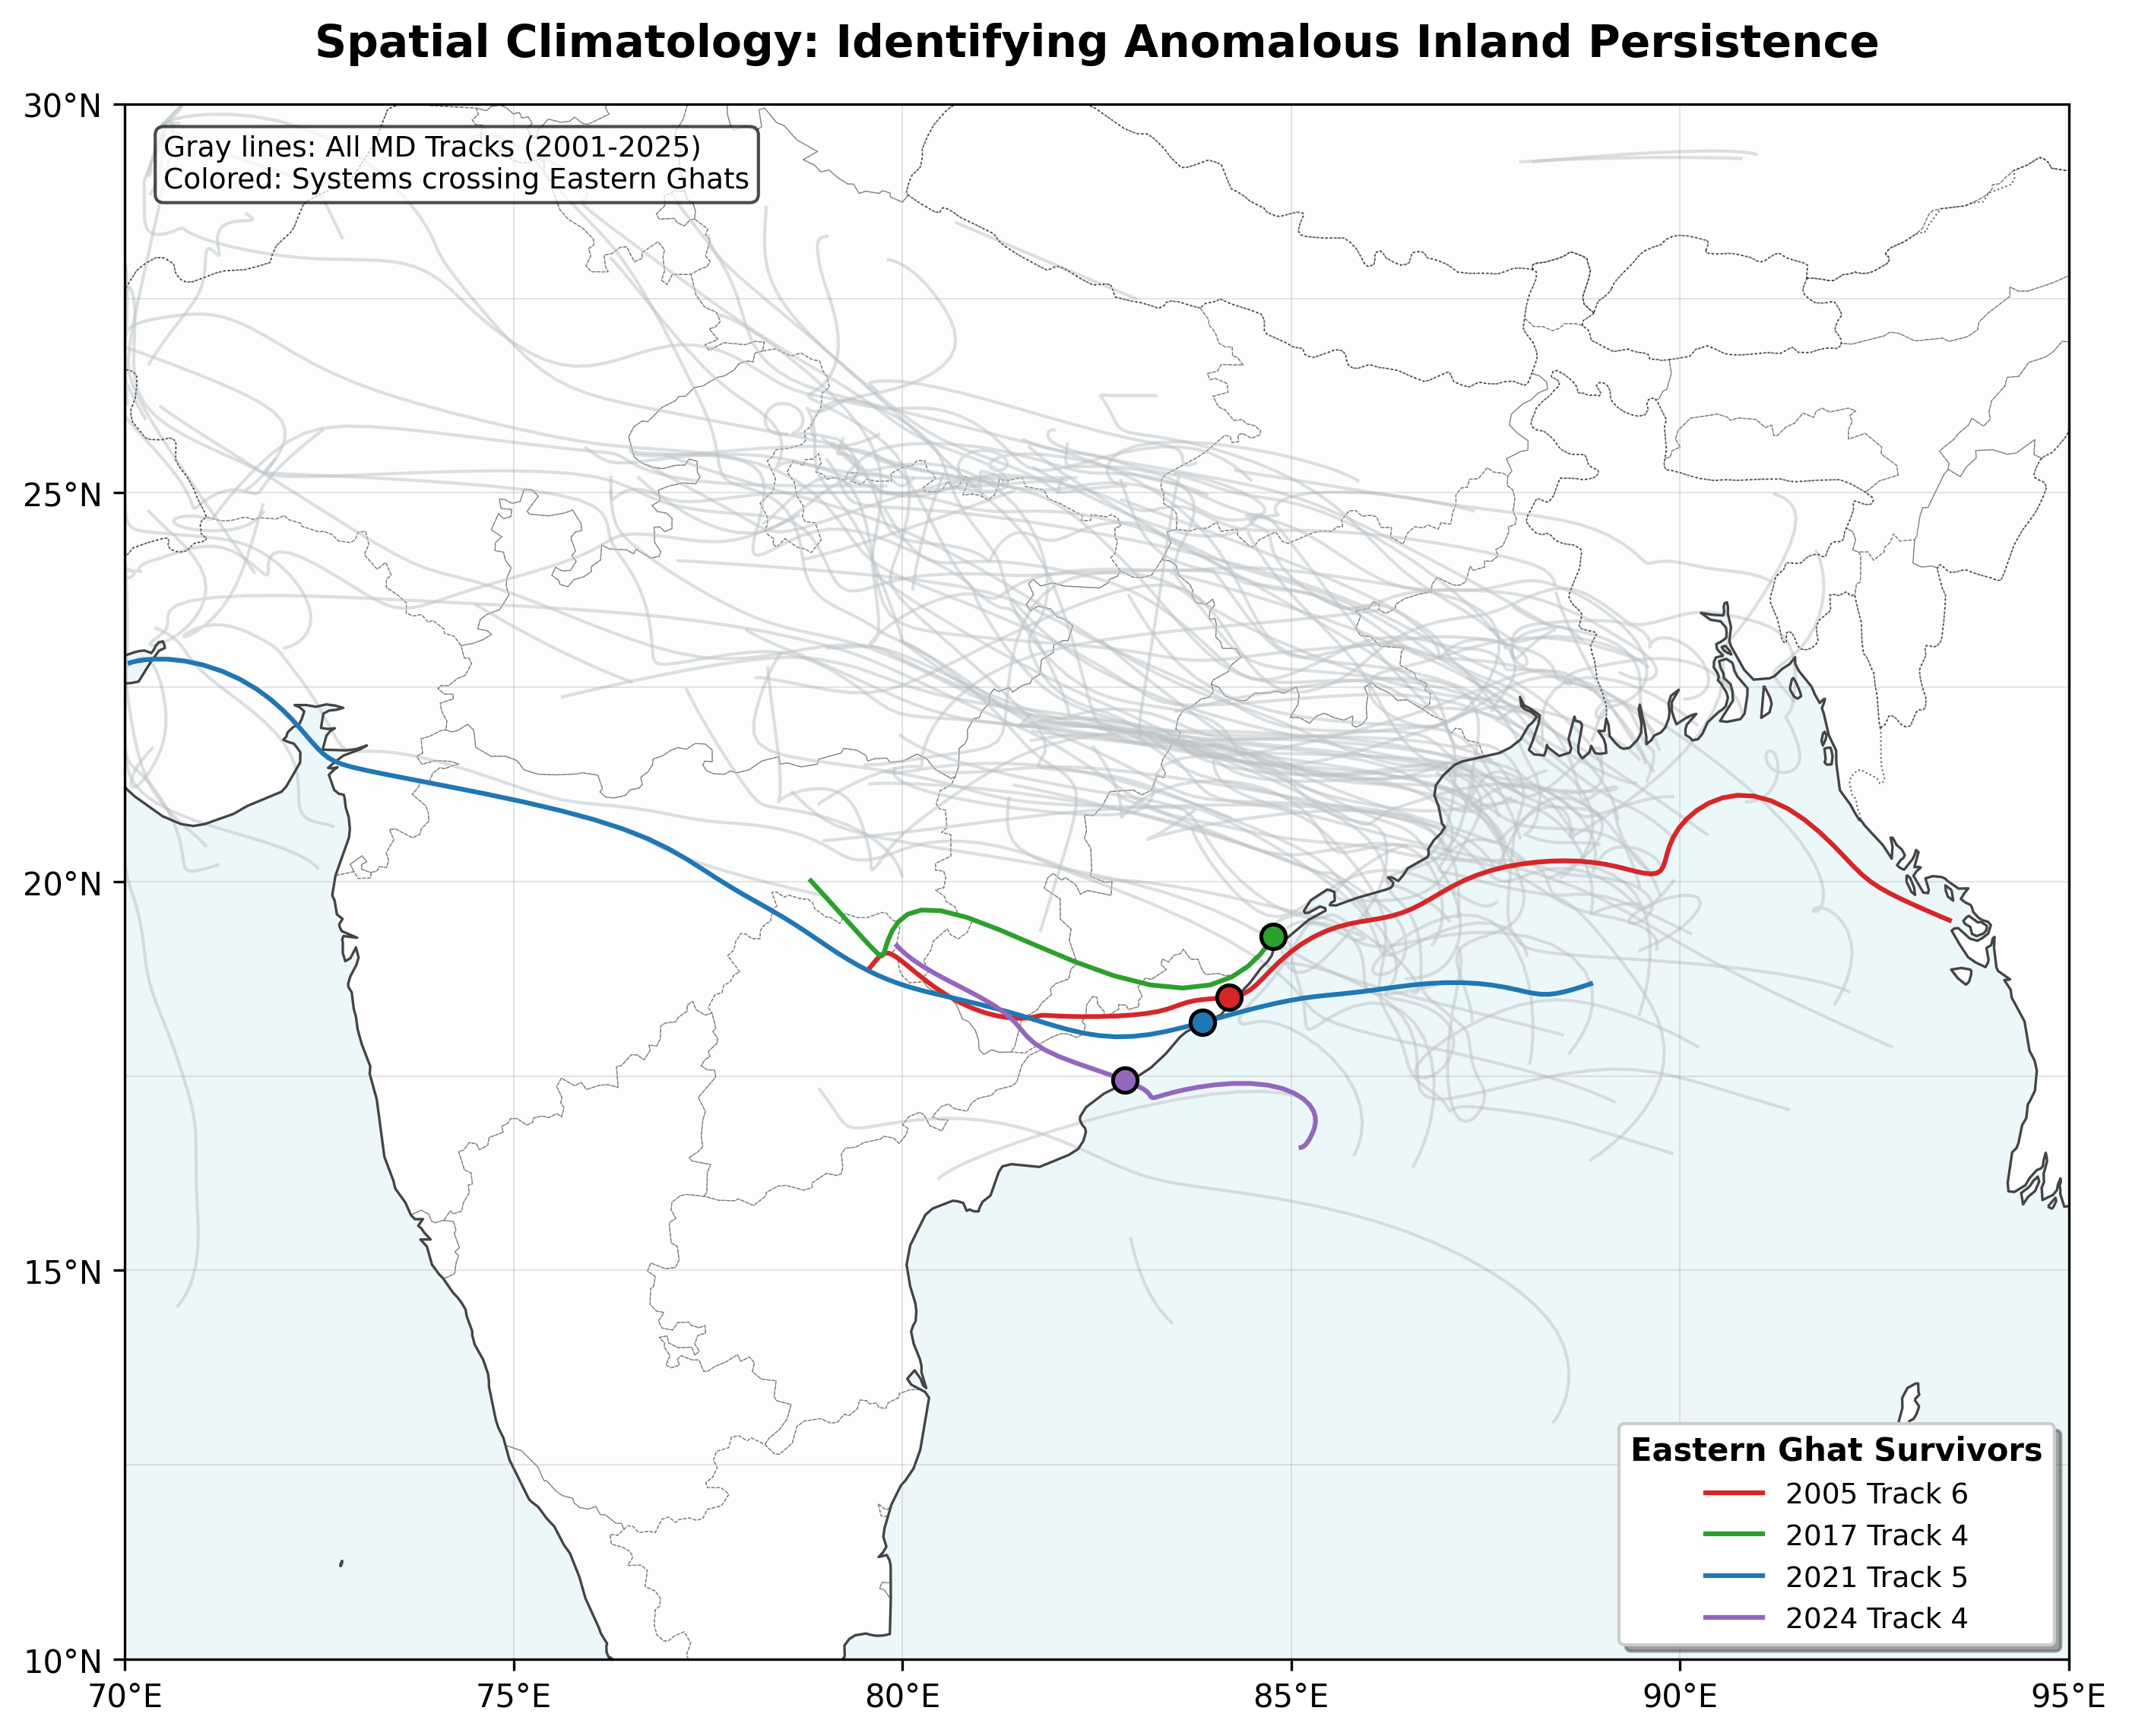
\includegraphics[width=0.95\textwidth]{ghats_survivors_map}
  \caption[Spatial distribution of Eastern Ghats
  survivors]{Comparison of standard MD tracks vs. the four anomalous
    survivor systems. Landfall points for survivors are marked with
    circles, indicating where the transition to Brown Ocean Effect
  thermodynamic maintenance begins.}
  \label{fig:ghats_survivors_map}
\end{figure}

The survival of these systems suggests that land-atmosphere coupling
(the BOE) provides sufficient energy to overcome the mechanical
frictional dissipation usually imposed by the Ghats.
